\chapter{$\zg$+Jets at the LHC}
\label{chap:Zs}

\section{Introducing $\zg$+Jets at the LHeqC}

	The work in this chapter is based on our recently published paper \cite{ZPaper}.
	The Large Hadron Collider (LHC)
	sheds ever more light on Standard Model processes at higher energies as it
	continues into Run II.  One ``standard candle'' process for the validation of
	the Standard Model description in this new energy regime is the production of
	a di-lepton pair through an intermediate $Z$ boson or photon, in
	association with (at least) two jets \cite{Chatrchyan:2011ne, Aad:2011qv,
	Chatrchyan:2013tna, Aad:2013ysa, Khachatryan:2014zya, Aad:2014rta,
	Khachatryan:2014dea}.  This final state can be entirely reconstructed from
	visible particles (in contrast to $pp\to \text{dijets plus}(W\to) e\nu$) making it a particularly
	clean channel for studying QCD radiation in the presence of a boson.
	Experimentally this process is indistinguishable from the production of a
	virtual photon which has decayed into the same products and we will consider
	both throughout.

	$W$ and $\zg$-production are excellent benchmark processes for investigating
	QCD corrections, since the mass of the boson provides a perturbative scale,
	while the event rates allow for jet selection criteria similar to those
	applied in Higgs boson studies. $W,\zg$-production in association with dijets
	is of particular interest, since in many respects it behaves like a dijet
	production emitting a weak boson (i.e. electroweak corrections to a QCD
	process rather than QCD corrections to a weak process). This observation
	means that a study of $W,\zg$-production in association with dijets is
	relevant for understanding Higgs-boson production in association with dijets
	(which in the gluon-fusion channel can be viewed as a Higgs-boson correction
	to dijet production). This process is interesting (e.g.~for $CP$-studies) in
	the region of phase space with large dijet invariant mass, where the
	coefficients in the perturbative series have logarithmically large
	contributions to all orders. As an example of the increasing importance of
	the higher orders, it is noted that the experimental measurement of the
	$N+1/N$-jet rate in $\zg$+jets increases from 0.2 to 0.3 after application of
	very modest \wbf-style selection cuts even at 7~TeV~\cite{Chatrchyan:2011ne,Aad:2011qv,Aad:2013ysa}.

	The current state-of-the-art for fixed-order calculations for this process is the
	next-to-leading order calculation of $\zg$ plus 4 jets by the BlackHat
	collaboration~\cite{Ita:2011wn}.
	While it has become standard to merge next-to-leading order QCD calculations
	with parton
	showers~\cite{Frixione:2002ik,Nason:2004rx,Frixione:2007vw,Alioli:2010xd,Frixione:2010wd,Alwall:2014hca},
	results for jet production in association with vector bosons have so far only appeared with up to two
	jets~\cite{Re:2012zi,Campbell:2013vha}.  Indeed, $W/Z+0-$, $1-$ and
	$2-$jet NLO samples have been merged with higher-order tree-level matrix
	elements and parton
	shower formulations~\cite{Hoeche:2012yf,Frederix:2015eii}. However, a parton shower cannot be expected to
	accurately provide a description of multiple hard jets from its resummation of
	the (soft and collinear) logarithms which are enhanced in the region of small
	invariant mass.  An alternative method to describe the higher-order
	corrections is instead to sum the logarithmic corrections which are enhanced at
	large invariant mass between the particles.  This is the approach pioneered by
	the High Energy Jets (HEJ) framework~\cite{Andersen:2009nu,Andersen:2009he}.
	Here, the hard-scattering matrix elements for a given process are supplemented
	with the leading-logarithmic corrections (in $s/t$) at all orders in
	$\alpha_s$. This approach has been seen to give a good description of dijet and
	$W$ plus dijet data at both the TeVatron~\cite{Abazov:2013gpa} and the
	LHC~\cite{Aad:2011jz,Chatrchyan:2012gwa,Chatrchyan:2012pb,Aad:2014pua,Aad:2014qxa}.
	In particular, these logarithmic corrections ensure a good description of $W$
	plus dijet-production in the region of large invariant mass between the
	two leading jets~\cite{Aad:2014qxa}. It is not surprising that standard
	methods struggle in the region of large invariant mass, since the
	perturbative coefficients receive large logarithmic corrections
	to all orders, and perturbative stability is guaranteed only once these are systematically summed.

	The purpose of this paper is to develop the treatment of such large QCD
	perturbative corrections within \hej to include the process of $\zg$ plus
	dijets. While this process has many features in
	common with the $W$ plus dijets process, one major difference is the
	importance of interference terms, both between different diagrams within the
	same subprocess (e.g. $qQ\to qQ(Z\to)e^+e^-$ with emissions off either the $q$ or
	$Q$ line) and between $Z$ and $\gamma^*$
	processes of the same partonic configuration. For processes with two quark
	lines, the possibility to emit the $\zg$ from both of these leads to profound
	differences to the formalism, since the $t$-channel momentum exchanged
	between the two quark lines obviously differs whether the boson emission is
	off line $q$ or $Q$. Furthermore, the interference between the two resulting
	amplitudes necessitates a treatment at the amplitude-level. \hej is
	formulated
	 at the amplitude-level, which, together with the matching to
	 high-multiplicity matrix-elements, sets it apart in the field of
	high energy
	logarithms\cite{Kuraev:1976ge,Balitsky:1978ic,Lonnblad:1992tz,Lavesson:2005xu,Jung:2000hk,Jung:2010si,Colferai:2010wu,Caporale:2012ih,Ducloue:2012bm}. The
	added complication over earlier \hej-formalism (and indeed in any
	BFKL-related study) by the interfering $t$-channels introduces a new structure of divergences in both real and virtual
	corrections, and therefore a new set of subtraction terms are needed, in
	order to
	organise the cancellation of these divergences. The matching to full
	high-multiplicity matrix elements puts the final result much closer to those
	of fixed order samples merged according to the shower
	formalism~\cite{Re:2012zi,Campbell:2013vha,Hoeche:2012yf,Frederix:2015eii}
	--- although of course the logarithms systematically controlled with \hej are
	different to those controlled in the parton shower formalism. In particular,
	\hej remains a partonic generator, i.e.~although it is an all-order
	calculation (like a parton shower), it is not interfaced to a hadronisation
	model. Initial steps in combining the formalism of \hej and that of a parton
	shower (and hadronisation) were performed in Ref.\cite{Andersen:2011zd}.

	We begin the main body of this article by outlining the construction of a
	High Energy Jets amplitude and its implementation in a fully flexible parton
	level Monte Carlo in the next section.  In section~\eqref{sec:Constructing} we
	derive the new subtraction terms which allows us to fully account for
	interference between the amplitudes. The subtraction terms allow for the
	construction of the all-order contribution to the process as an explicit
	phase-space integral over any number of emissions. Specifically, the
	main result for the all-order summation is formulated in
	Eqn.~\eqref{eq:sigma}:
	\begin{align}
	  \nonumber
	  \begin{split}
	    \sigma =& \sum_{f_a,f_b} \sum_{n=2}^\infty \int \frac{d^3 p_a}{(2\pi)^3 2E_a} \int \frac{d^3
	      p_b}{(2\pi)^3 2E_b}  \left( \prod_{i=2}^n \int_{p_{i\perp}>\lambda_{cut}} \frac{d^3 p_i}{(2\pi)^3
	        2E_i} \right)\ (2\pi)^4 \delta^{(4)}\left(p_a+p_b - \sum_i p_i\right) \\
	    & \ \times \ |\mathcal{M}^{HEJ-{\rm reg}}_{f_af_b\to \zg
	      f_a(n-2)gf_b}(p_a,p_b,\{p_i\})|^2 \ \frac{ x_a f_{f_a}(x_a, Q_a) x_b
	      f_{f_b}(x_b,Q_b)}{\hat s^2}\ \Theta_{\rm cut},
	  \end{split}
	\end{align}
	where $\sigma$ is the sough-after cross
	section, and the rest of the equation is discussed in the relevant section. Section~\eqref{sec:Constructing} also discusses the necessary
	modifications in order to include fixed-order matching. In
	section~\eqref{sec:Comparisons} we show and discuss the comparisons between the new
	predictions obtained with \hej and LHC data. We conclude and present the
	outlook in section~\eqref{Conclusions}.

\section{Constructing $\zg$+jets}
	\label{sec:Zcurrents}

	\subsection{A Current for $Z^0$+Jets}

		For any given initial state (excluding the case of gluon-gluon scattering which will
		not contribute an FKL configuration) there are two possible emission sites for the
		$Z^0$ per fermion i.e. two for $qg$ and $\bar qg$ scattering and four for $qq$,
		$\bar qq$ and $\bar q\bar q$ scattering. The emission sites on a single fermion line
		are illustrated in fig. \eqref{fig:emissionsites}.  In the language of currents discussed
		previously we call the left hand side of fig. \eqref{fig:emissionsites} $j_\mu^\zg$.
		It is given by:

		\begin{align}
		  \begin{split}
		    j^Z_\mu = \frac{C_{Zq}C_{Ze}}{p_Z^2 - M^2_Z +
		      i\Gamma_ZM_Z}\Big(&\frac{\bk{1}{\gu{\sigma}(\slashed p_{out} + \slashed
		        p_{e^+} + \slashed p_{e^-})\gl{\mu}}{a}}{(p_{out} + p_Z)^2} + \\
		    &\frac{\bk{1}{\gu{\mu}(\slashed p_{in} - \slashed p_{e^+} - \slashed
		        p_{e^-})\gl{\sigma}}{a}}{(p_{in} - p_Z)^2}\Big)\bk{e^+}{\gl{\sigma}}{e^-},
		    \label{eqn:Zcurrent}
		  \end{split}
		\end{align}

		\begin{figure}[bt]
			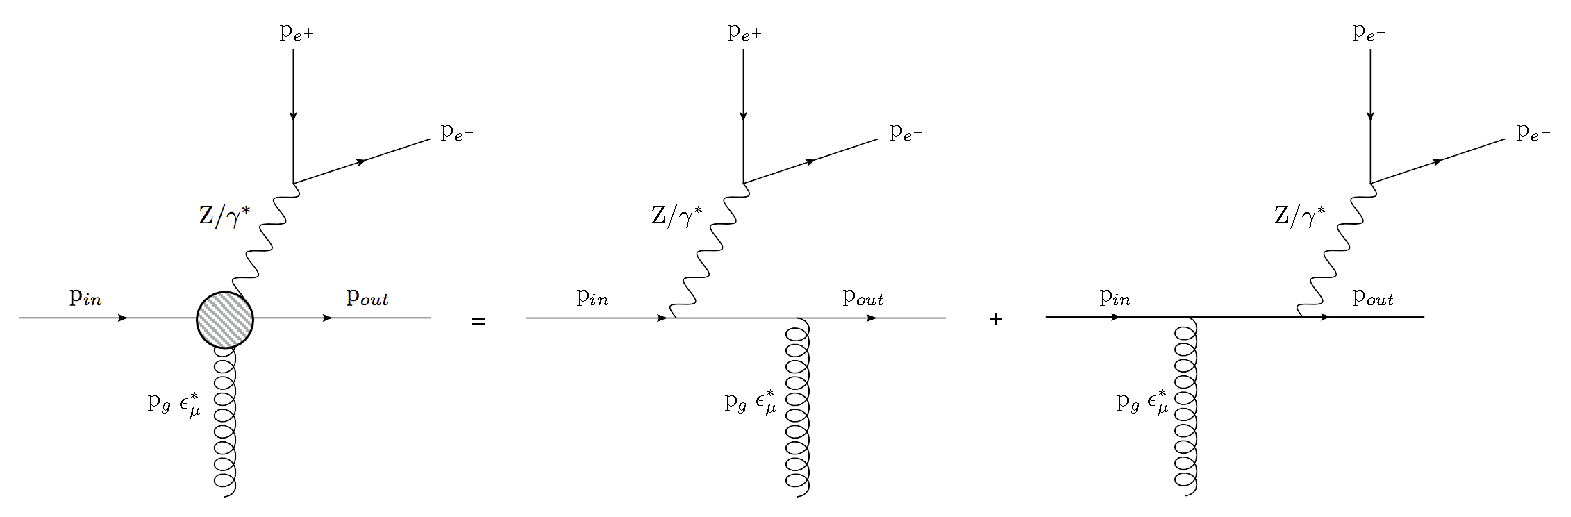
\includegraphics[width=0.98\linewidth]{figures/EmissionSites.pdf}
			\caption{The possible emission sites for a neutral weak boson.}
			\label{fig:emissionsites}
		\end{figure}

		where $M_Z$ is the mass of the $Z$ boson, $\Gamma_Z$ is its width, $C_{Zx}$ is
		the coupling of the $Z$ to $x$, $x=e,q,\nu_e,\ldots$ and $\mu$ is the Lorentz
		index for the $t$-channel gluon propagator.

		We can expand the quark and lepton momenta using their completeness relations which,
		in terms of spinor-helicity brackets, is given by:

		\begin{equation}
			\slashed p_{i} = |i_+\rangle\langle i_+| + |i_-\rangle\langle i_-|.
		\end{equation}

		We can fix the helicity of the incoming quark, $h_{in}$, and the outgoing quark,
		$h_{out}$, to be identical, and we are left with a current which only has four
		possible helicity configurations depending on $h_q = h_{in} = h_{out}$ and the
		electron helicity, $h_e$:

		\begin{align}
		  \begin{split}
		    j^Z_\mu(h_q, h_e) = &\ C_{Zq}^{h_q}C_{Ze}^{h_e}\ \frac{\bk{e^+_{h_e}}{\gl{\sigma}}{e^-_{h_e}}}{p_Z^2 -
		      M^2_Z + i\Gamma_ZM_Z} \\ &\ \times\bigg(\frac{2p_1^\sigma\bk{1_{h_q}}{\gu{\mu}}{a_{h_q}} +
		      \bk{1_{h_q}}{\gu{\sigma}}{e^+_{h_q}} \bk{e^+_{h_q}}{\gu{\mu}}{a_{h_q}} +
		      \bk{1_{h_q}}{\gu{\sigma}}{e^-_{h_q}} \bk{e^-_{h_q}}{\gu{\mu}}{a_{h_q}}}
		    {(p_{out} + p_Z)^2}\\
		    &\qquad + \frac{ 2p_a^\sigma\bk{1_{h_q}}{\gu{\mu}}{a_{h_q}} -
		      \bk{1_{h_q}}{\gu{\mu}}{e^+_{h_q}} \bk{e^+_{h_q}}{\gu{\sigma}}{a_{h_q}} -
		      \bk{1_{h_q}}{\gu{\mu}}{e^-_{h_q}} \bk{e^-_{h_q}}{\gu{\sigma}}{a_{h_q}}}
		    {(p_{in} - p_Z)^2}\bigg).
		    \label{eq:Zcurrent}
		  \end{split}
		\end{align}

		We can then express amplitudes for $Z^0$ plus jets in terms of contractions of
		a Z emitting and either a quark or gluon current discussed previously.  Taking
		the concrete example of $qg\to Zqg$ we can write the matrix element as follows:

		\begin{align}
		\begin{split}
			{|\bar{\mathcal{M}}_{qg\to Zqg}^{t}|}^2 =& \ \frac{g_s^2}{8}\
			\frac{1}{(p_a-p_1-p_{e^+}-p_{e^-})^2 (p_b-p_n)^2}  \sum_{h_q,h_e,h_g}|
			j^{Z}_\mu(h_q,h_e) j^{g\mu}(h_g)|^2.
		  	\label{eq:qgamp}
		\end{split}
		\end{align}

		If we investigate eqn. \eqref{eq:qgamp} for a `slice' through the final state phase-space
		where each particles momenta is parametrised by:

		\begin{align}
		\begin{split}
			p_i = &k_{i\perp}\Big(\cosh (y_i); \cos (\phi_i), \sin (\phi_i), \sinh (y_i)\Big) \\
			\intertext{and,}
			k_{1\perp} = k_{e^+\perp} = 40\mbox{GeV}& \hspace{0.5cm} k_{e^-\perp} =
			\frac{m_Z^2}{2k_{e^+\perp}\left(\cosh(y_{e^+} - y_{e^-}) -
			    \cos(\varphi_{e^+} - \varphi_{e^-}))\right)}, \\
			\varphi_{1} =& \pi \hspace{0.5cm} \varphi_{e^+} = \pi + 0.2 \hspace{0.5cm}
			\varphi_{e^-} = -(\pi + 0.2), \\
			y_1=\Delta& \hspace{0.5cm} y_2=-\Delta \hspace{0.5cm} y_{e^+} = \Delta
			\hspace{0.5cm} y_{e^-} = \Delta - 1.5.
			\label{eq:momenta}
		\end{split}
		\end{align}

		Then we observe the behaviour shown in fig. \eqref{fig:ZatLO}: as we pull the
		jets apart in rapidity (i.e. as we go to large $\Delta$) we see that the matrix element
		approaches a constant; this is the result which would be obtained by using the BFKL
		formalism in which all jets are taken be infinitely well separated in rapidity.\\As we
		expect for the case of $2\to 2$ scattering we see exact agreement between our expression
		and the leading order result obtained from \texttt{MadGraph5} \cite{Alwall:2014hca}.

		\begin{figure}[hbt]
			\centering
			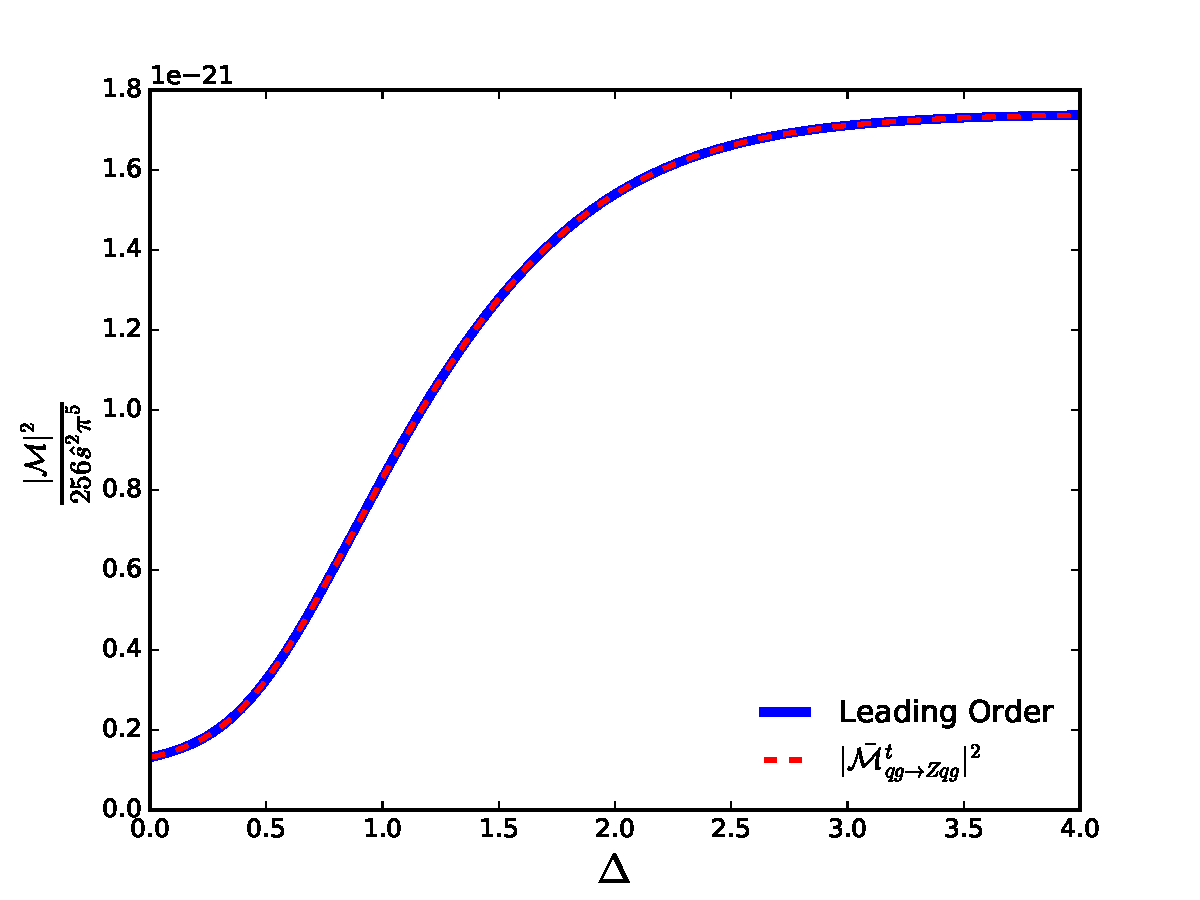
\includegraphics[width=1.0\linewidth]{Z_NoI_qg.pdf}
			\caption{$\overline{|\mathcal{M}_{qg\to Zqg}^{t}|}^2$ shown for a slice through the
			final state phase-space defined by eqn. \eqref{eq:momenta}.  We compare to the
			leading order result obtained from \texttt{MadGraph}.}
			\label{fig:ZatLO}
		\end{figure}

		The picture becomes more complicated when considering the $qQ\to ZqQ$ scattering since,
		as mentioned previously, there are four possible places where the (anti-)quark may emit
		the $Z^0$.  In previous work by the High Energy Jets collaboration the case of
		$W^\pm$ plus multiple hard jets was treated by simply attaching the boson to an external
		quark line probabilistically \cite{Andersen:2012gk}.  However as we will see later this
		leads to an approximate matrix element which differs significantly from the leading-order
		result and so here we will include not only the contributions to the matrix element arising
		from the $Z^0$ being emitted from both (anti-) quark legs separately but also the resulting
		interference term.

	\subsection{$Z^0$ Emission Interference}

		Our high-energy
		description of the matrix elements relies on the correct description of the
		$t$-channel momenta, and this obviously depends on which of the quark lines
		the $Z$ or $\gamma^*$ was emitted from.  We therefore need to modify the simple
		framework outlined above.  We will use the subscript $a$ ($b$) to label the
		current at the lowest (highest) end of the rapidity chain.  We then define $t_a$
		($t_b$) to be the $t$-channel momentum exchanged when the bosons are emitted at
		the lowest (highest) end of the rapidity chain.  Then the full amplitude squared
		for $qQ\to qQ(\zg\to) e^+ e^-$ is given by:

		\begin{align}
		\begin{split}
			{|\bar{\mathcal{M}}_{qg\to Zqg}^{t}|}^2 &= g_s^2 \frac{C_F}{8N_c}
			\Big|\frac{j^{Z^0}_a\cdot j_b}{t_a} + \frac{j_a\cdot
			j^{Z^0}_b}{t_b}\Big|^2\\
			&= g_s^2 \frac{C_F}{8N_c} \left( \Big|\frac{j^{Z^0}_a\cdot j_b}{t_a}\Big|^2 + \Big|\frac{j_a\cdot
			j^{Z^0}_b}{t_b}\Big|^2 + 2\Re{\Big\{\Big(\frac{j^{Z^0}_a\cdot
			j_b}{t_a}\Big)\Big(\frac{j_a\cdot j^{Z^0}_b}{t_b}\Big)^*\Big\}} \right),
			\label{eqn:interference}
		\end{split}
		\end{align}

		where $j_{a,b}$ are the pure quark currents defined previously.  The
		coupling constants of the $Z$ to the relevant quarks and leptons are contained
		within $j^{Z^0}(h_q,h_e)$, as in eqn.~(\eqref{eqn:Zcurrent}).  Fig.~\eqref{fig:twojets}
		shows the value of this matrix element squared divided by the squared partonic
		centre-of-mass energy for increasing rapidity separation of the two jets. Once again the
		result is compared with that obtained from the full, tree-level matrix elements from
		\texttt{MadGraph5}.

		The slice through phase space here is the same as that used in the previous
		section given by eqn. \eqref{eq:momenta}.  Fig.~\eqref{fig:twojets} also shows
		the separate contributions to the total matrix element squared coming from the
		$\zg$ emission from the forward moving quark line (black, dashed) and emission
		from the backward moving quark line (green, dotted).  In this phase space slice,
		the leptons also have an increasing positive rapidity and so the forward emission
		matrix element describes the full matrix element most closely, with the contribution
		from backward-emission falling at large values of $\Delta y$.  The sum of the forward
		and backward emission matrix elements neglecting interference (magenta, dotted)
		significantly overestimates the final result.  Once the destructive interference
		effects have been taken into account, the full sum (red, solid) correctly reproduces
		the LO matrix element (blue, thick solid).  It is therefore clear that at low
		rapidities the inclusion of the interference effect plays an important role in
		the accuracy of the matrix element.  This important interference effect is not
		included in descriptions when electroweak corrections are included in a parton
		shower~\cite{Christiansen:2014kba,Krauss:2014yaa,Christiansen:2015jpa}.

		\begin{figure}[hbt]
		  \begin{center}
		    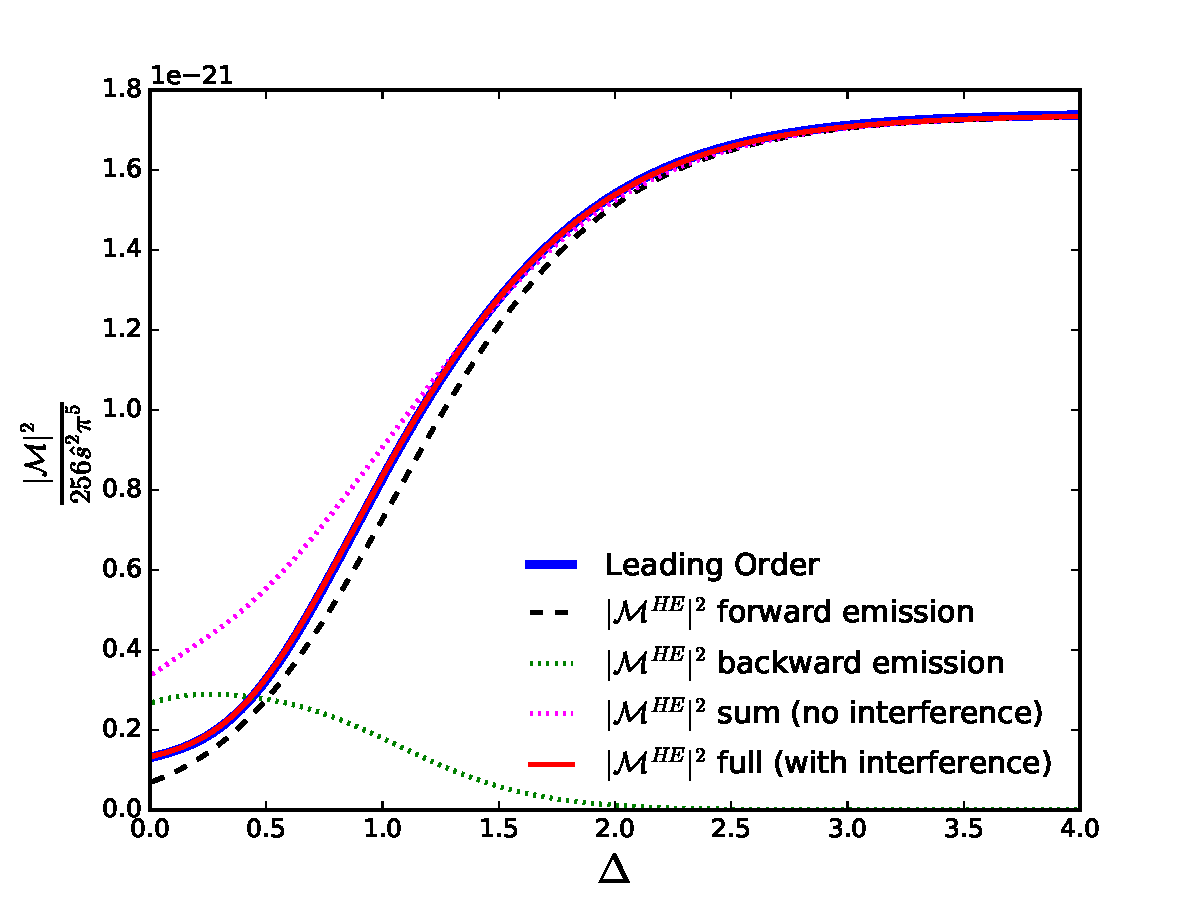
\includegraphics[width=1.0\linewidth]{slice.pdf}
		    \caption{The matrix-element squared divided by the square of the partonic
		      centre-of-mass energy for $qQ\to ZqQ$ with the $Z$ decaying to an
		      electron-positron pair for the phase space slice described in
		      eqn.~\eqref{eq:momenta}.  Increasing values of $\Delta$ represent
		      increasing rapidity separation between the jets.  The different lines show the contributions from
		      different terms in the calculation: only emission from the forward or the
		      backward quark line (black, dashed and green, dotted), their sum without
		      the interference term (magenta, dotted) and their sum including
		      interference (red, solid) which is seen to agree exactly with the LO result
		      (blue, thick solid).}
		    \label{fig:twojets}
		  \end{center}
		\end{figure}

	\subsection{Photonic Interference}

		Since any virtual $Z^0$ could also have proceeded via an off-shell virtual photon,
		$\gamma^*$, we must also include these processes and the resulting interference the
		$Z^0$ and $\gamma^*$.\\
		The $\gamma^*$ emission matrix element is similar to that of the $Z^0$-only matrix
		element shown in equation \eqref{eq:qgamp} and the same story applies with the
		possible emission sites causing interference.  All that needs to be changed is the
		propagator term and the couplings of the boson to the emitting (anti-)quark and
		the decay products.  The full current for $\zg$ emission is then obtained by summing
		the two separate currents as follows:

		\begin{align}
			\label{eq:jsum}
			j^{\zg}_\mu(h_q,h_e) = j^Z_\mu(h_q,h_e) + j^\gamma_\mu(h_q,h_e).
		\end{align}

		Then upon squaring eqn. \eqref{eq:jsum} we will automatically include the interference
		terms from the cross-terms. The inclusion of the virtual photon terms is particularly
		important when studying a combined lepton invariant mass, $(p_{e^+} + p_{e^-})^2$,
		far from the $Z$ Breit-Wigner mass peak. This can be seen in fig. \eqref{fig:DileptonMass},
		where slices through phase space are shown similarly to fig. \eqref{fig:twojets}, but
		now for an (a) lower and (b) higher value of the di-lepton mass.  In both cases, the
		contribution of the virtual photon processes is above 25\%.

		\begin{figure}[hbtp]
		        \centering
		        \begin{subfigure}[b]{0.82\textwidth}
		                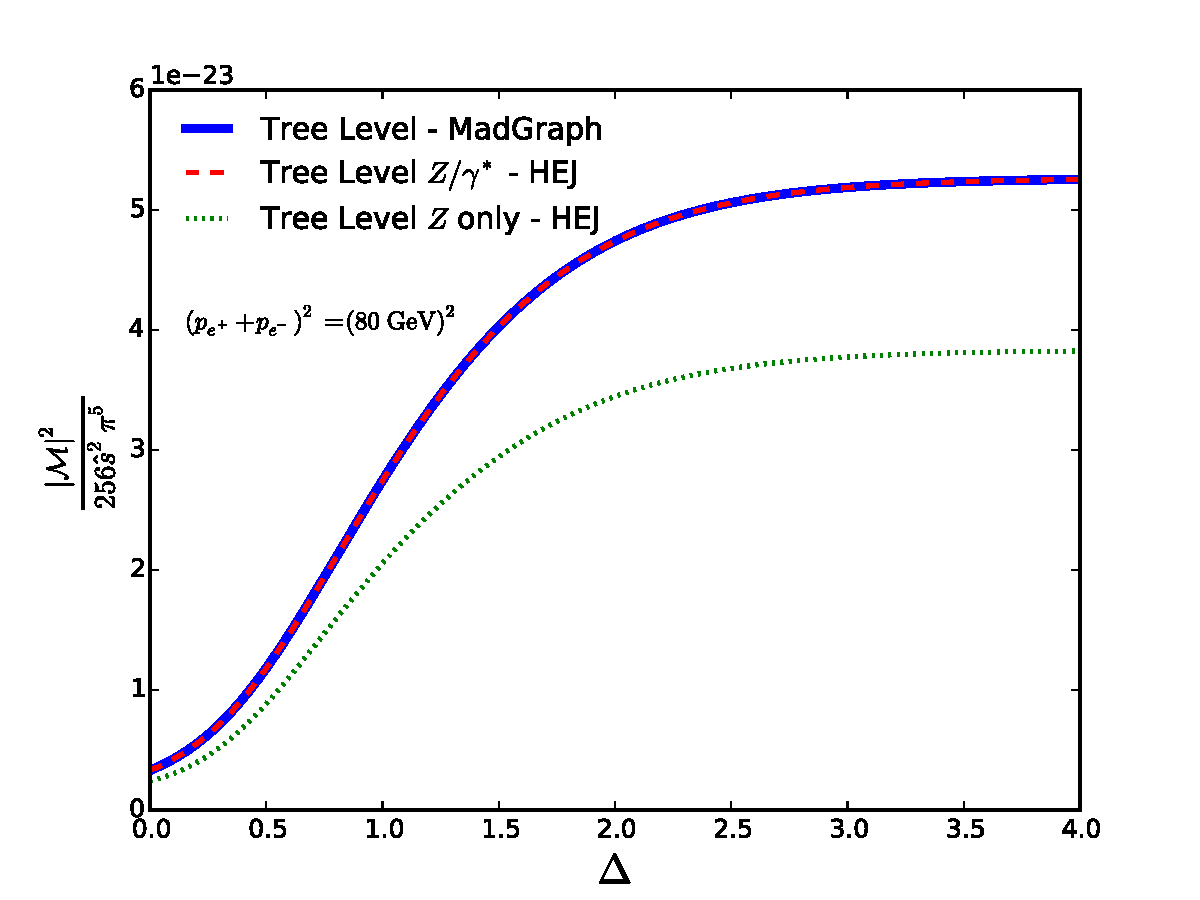
\includegraphics[width=\textwidth]{ZLowMass}
		                \caption{}
		                \label{fig:LowDileptonMass}
		        \end{subfigure}
		        ~
		        \begin{subfigure}[b]{0.82\textwidth}
		                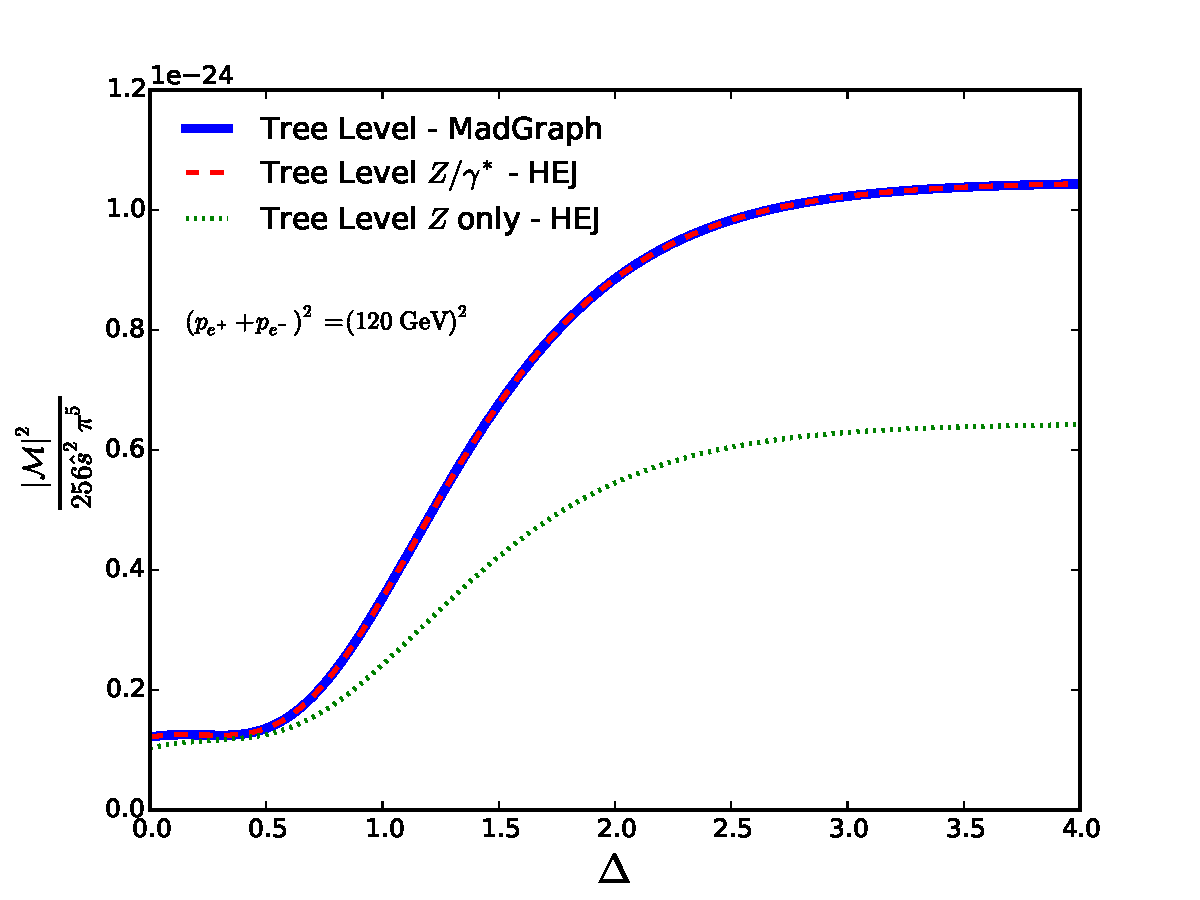
\includegraphics[width=\textwidth]{ZHighMass}
		                \caption{}
		                \label{fig:HighDileptonMass}
		        \end{subfigure}
		        \caption{The matrix-element squared divided by the square of the
		          partonic centre-of-mass energy for $qQ\to \zg qQ$ with the $\zg$ decaying
		          to an electron-positron pair.  The
		          $\mathcal{O}(\alpha_s^2 \alpha_W)$ tree-level contribution
		          as described in HEJ (red, dashed) exactly matches that of
		          \texttt{MadGraph5} (blue, solid).  The terms corresponding to the production
		          of a $Z$ boson only (green, dotted) significantly undershoots the
		          full result.  The
		          virtual photon terms are, therefore, clearly an important
		          contribution to the matrix element away from the $Z$ Breit-Wigner
		          peak.}
		        \label{fig:DileptonMass}
		\end{figure}

	\subsection{The $2\rightarrow n$ Matrix Element}

		Armed with \eqref{eq:jsum} we can extend eqn. \eqref{eq:qgamp} in the obvious way
		to form a complete matrix element for the emission of a $\zg$ boson.  We can also
		describe the various possibilities ($qq$, $qg$ and $gq$) simply by substituting
		the currents which apply in any given situation.  Of course, in practise we use
		the importance sampling techniques discussed in chapter \ref{chap:HEQCD} to
		randomly sample the possible incoming parton types and so all combinations of
		currents are required.\\Following in the vein of the previous chapter we now look
		to extend our description to higher multiplicity final states.  Based on eqn.
		\eqref{eqn:factorised2ToN} from chapter \ref{chap:HEQCD} we can write the squared
		matrix element for $qQ\to (\zg\to ) e^+e^- q (n-2)g Q$ is:

		\begin{align}
		\begin{split}
		    |\mathcal{M}^{t}_{qQ\to \zg q(n-2)gQ}|^2 = &g_s^2 \frac{C_F}{8N_c}\ ( g_s^2
		    \Ca)^{n-2}\  \\  \times \Bigg(& \frac{| j_a^{\zg}\cdot j_b|^2}{t_{a1}t_{a(n-1)}} \prod^{n-2}_{i=1} \frac{-V^2(q_{ai},
		      q_{a(i+1)})}{t_{ai} t_{a(i+1)}}+\ \frac{|j_a \cdot j_b^{\zg} |^2}{t_{b1}t_{b(n-1)}}
		    \prod^{n-2}_{i=1}\frac{-V^2(q_{bi}, q_{b(i+1)})}{t_{bi} t_{b(i+1)}}  \\
		    &- \frac{2\Re\{(j_a^{\zg}\cdot j_b)(\overline{j_a \cdot
		        j_b^{\zg}})\}}{\sqrt{t_{a1}t_{b1}}\sqrt{t_{a(n-1)} t_{b(n-1)}}}
		    \prod^{n-2}_{i=1}\frac{V(q_{ai}, q_{a(i+1)})\cdot V(q_{bi},
		      q_{b(i+1)})}{\sqrt{t_{ai}t_{bi}} \sqrt{t_{a(i+1)}t_{b(i+1)}}}\Bigg).
			\label{eq:allorderreal}
		\end{split}
		\end{align}

		In the case of $n=2$, this reduces back to eqn.~(\ref{eqn:interference}).  If
		either $a$ or $b$ is an incoming gluon, there is once again a unique set of
		$t$-channel momenta and one can set the relevant $j_a^{\zg}$ or $j_b^{\zg}$ to
		zero in the formula above.\\Eqn.~(\ref{eq:allorderreal}) gives us the all-orders
		real corrections to $\zg$ plus jets.  However, before proceeding to calculate the
		cross-section we must carefully render eqn. (\ref{eq:allorderreal}) finite by
		including the virtual corrections whose divergences will cancel the pathologies
		in the effective vertices.

\section{Regularising the $\zg$+Jets Matrix Element}
	\label{sec:regularising}

	\subsection{Real Soft Emissions}
		\label{sub:softEmissions}

		To calculate useful quantities such a cross sections etc. we must integrate equation
		\eqref{eq:allorderreal} over all of phase space.  However, as discussed in chapter \ref{chap:theory}
		problems arise when we attempt to integrate over the soft regions of phase space.  It is well understood
		that the divergences coming from soft real emissions cancel with those coming from soft
		virtual emissions and so we must explicitly show this cancellation and calculate the remaining
		finite contribution multiplying the $(n-1)$-final state parton matrix element.\\
		In the previous work on $W^\pm$ emission the finite contribution was found to be
		\cite{Andersen:2009nu, Andersen:2008gc}:

		\begin{equation}
			\frac{\alpha_s C_a \Delta_{j-1, j+1}}{\pi}\ln{\frac{\lambda_{cut}^2}{|\vec{q}_{j\perp}|^2}},
		\end{equation}

		where $\Delta_{i-1, i+1}$ is the rapidity span of the final state partons either side of our
		soft emission and $|\vec{q}_{j\perp}|^2$ is the sum of squares of the transverse components of
		the $j^{th}$ $t$-channel gluon momenta.  $\lambda_{cut}$ is a parameter we choose which \emph{defines}
		the soft region.  I.e. any real emission satisfying $p^2 \geq \lambda_{cut}^2$ we consider a hard perturbative
		emission while any emission with $p^2 < \lambda_{cut}^2$ we consider too soft to be resolved.\\
		Here we investigate
		the cancellation of these divergences for $Z$ emission and most importantly whether the finite term
		is of the same form for the interference term which was previously excluded.\\We start by looking
		at a $2\rightarrow n$ process and take the limit of one final state parton momentum, $p_i$, becoming
		small.  Because of the form of eqn. \eqref{eq:allorderreal} this amounts to looking at the
		effect of an external gluon becoming soft on eqn. \eqref{eqn:unsymm} (an identical - though
		longer - calculation also holds for the symmetrised version of the effective vertex), we can
		immediately see that for $p_i$ going soft the gluon `chain' momenta going into,
		and coming out of, the $j^{th}$ emission site will coincide: $q_{j+1}\sim q_j$:

		\begin{equation}
			V^\rho(q_j, q_{j+1}) \rightarrow -2q_j^\rho - 2\left(\frac{s_{aj}}{s_{ab}} -
				\frac{q^2_{j}}{s_{bj}}\right)p_b^\rho + 2\left(\frac{s_{bj}}{s_{ab}} +
				\frac{q_j^2}{s_{aj}}\right)p_a^\rho
				\label{eqn:vertexlimit}
		\end{equation}

		In eqn. \eqref{eq:allorderreal} we have three terms involving the effective vertex;
		quadratic terms like $V^2(q_{tj}, q_{t(j+1)})$ and $V^2(q_{bj}, q_{b(j+1)})$ and interference terms
		like $V(q_{tj}, q_{t(j+1)})\cdot V(q_{bj}, q_{b(j+1)})$.  The procedure for the $V^2$ terms follows
		similarly for both the quadratic top-line emission and bottom-line emission terms and so only
		the calculation for top-line emission is shown here.

		\subsubsection{$V^2(q_{tj}, q_{t(j+1)})$ Terms}

			Once we square eqn. \eqref{eqn:vertexlimit} and impose the on-shell conditions for
			$p_a$ and $p_b$ we get:

			\begin{align}
				V^2(q_{tj}, q_{tj}) = &4q_j^2 + 8 q_j\cdot p_b \left(\frac{s_{aj}}{s_{ab}} - \frac{q^2_{j}}{s_{bj}}\right) -
					8q_j\cdot p_a \left(\frac{s_{bj}}{s_{ab}} + \frac{q_j^2}{s_{aj}}\right) \\ &- 4s_{ab}\left(\frac{s_{aj}}{s_{ab}} -
					\frac{q^2_{j}}{s_{bj}}\right)\left(\frac{s_{bj}}{s_{ab}} + \frac{q_j^2}{s_{aj}}\right).
			\end{align}

			Since $p_j\rightarrow0$ the dot-products $s_{aj}$ and $s_{bj}$ will also become small,
			therefore:

			\begin{equation}
				V^2(q_{tj}, q_{tj}) = 4q_j^2 + 8 q_j\cdot p_b \frac{q^2_{j}}{s_{bj}} - 8 q_j\cdot p_a \frac{q_j^2}{s_{aj}} -
					4s_{ab}\frac{q^4_{j}}{s_{bj}s_{aj}}.
			\end{equation}

			Clearly the final term now dominates due to its $\sim\frac{1}{p_i^2}$ behaviour and so
			in the soft limit we have:

			\begin{equation}
				V^2(q_{ti}, q_{ti}) = - \frac{4s_{ab}}{s_{bi}s_{ai}}q^4_{i} + \mathcal{O}\left(\frac{1}{|p_i|}\right).
				\label{eqn:temp}
			\end{equation}

			We must now explicitly calculate the invariant mass terms.  Since we are in the
			High Energy regime we may take:

			\begin{align}
				p_a\sim p_1 \sim p_+ = \Big(\frac12 p_z, 0, 0, \frac12 p_z\Big),\\
				\intertext{and,}
				p_b\sim p_n \sim p_- = \Big(\frac12 p_z, 0, 0, -\frac12 p_z\Big).
			\end{align}

			We describe our soft gluon with $p_i=(E, \vec{p})$ and therefore we may express the
			products of momenta as follows:

			\begin{align}
				s_{ai} &= 2p_a\cdot p_i\sim2p_+\cdot p_i = \frac12p_zE - \frac12p_z^2,\\
				s_{bi} &= 2p_b\cdot p_i\sim2p_-\cdot p_i = \frac12p_zE + \frac12p_z^2,\\
				s_{ab} &= \frac12p_z^2.
			\end{align}

			Using these to calculate only the leading divergence in eqn. \eqref{eqn:temp} reads:

			\begin{subequations}
				\begin{equation}
				V^2(q_{ti}, q_{ti}) = - \frac{4p_z^2}{(p_zE - p_z^2)(p_zE + p_z^2)}q^4_{i} + \mathcal{O}\left(\frac{1}{|p_i|}\right),
				\end{equation}
				\begin{equation}
				V^2(q_{ti}, q_{ti}) = - \frac{4p_z^2}{p_z^2(E^2-p_z^2)}q^4_{i} + \mathcal{O}\left(\frac{1}{|p_i|}\right),
				\end{equation}
			\end{subequations}

			but since $E^2-\vec{p}_1^2=0$ for the on-shell external parton this can be written as:

			\begin{equation}
				V^2(q_{ti}, q_{ti}) = - \frac{4}{|\vec{p}_{1\perp}|^2}q^4_{i} + \mathcal{O}\left(\frac{1}{|p_i|}\right),
				\label{eqn:temp2}
			\end{equation}

			Now looking back to eqn. \eqref{eq:allorderreal} we see that each vertex is associated with factors of
			$q^{-2}_{ti}q^{-2}_{t(i+1)}$ but since the emission is soft this becomes $q^{-4}_{ti}$.
			That factor conspires to cancel with the corresponding factor in eqn. \eqref{eqn:temp2},
			Including the addition factors of $C_A$ and $g_s$ dropping any sub-leading divergences, the finite factor remaining is given by:

			\begin{equation}
				\frac{4C_Ag_s^2}{|\vec{p}_\perp|^2},
				\label{eqn:finalsoft}
			\end{equation}

		\subsubsection{$V(q_{ti}, q_{t(i+1)})\cdot V(q_{bi}, q_{b(i+1)})$ Terms}
			\label{sub:subsection_name}

			The calculation of the interference term with a soft emission follows similarly to
			that in above section. After taking $p_i\rightarrow0$ and taking the dot-product of
			the two vertex terms together we have:

			\begin{equation}
			\begin{split}
				V(q_{ti}, q_{ti})\cdot V(q_{bi}, q_{bi}) =
				4q_i^t\cdot q_i^b &- 4q_i^t\cdot p_a\left(\frac{s_{bi}}{s_{ab}} +
				\frac{t_i^b}{s_{ai}}\right) + 4q_i^t\cdot p_b\left(\frac{s_{ai}}{s_{ab}} +
				\frac{t_i^b}{s_{bi}}\right)\\
				&- 4q_i^b\cdot p_a\left(\frac{s_{bi}}{s_{ab}} + \frac{t_i^t}{s_{ai}}\right) +
				4q_i^b\cdot p_b\left(\frac{s_{ai}}{s_{ab}} +
				\frac{t_i^t}{s_{bi}}\right),\\
			\end{split}
			\end{equation}

			having simplified the expression using $p_a^2=0$ and $p_b^2=0$ once again.  We may
			drop all the terms with $s_{ai}$ or $s_{bi}$ in the denominator and this time we are
			left with two terms which contribute.  They combine to give:

			\begin{equation}
				V(q_{ti}, q_{ti})\cdot V(q_{bi}, q_{bi}) = -\frac{s_{ab}}{s_{ai}s_{bi}}t_i^tt_i^b +
					\mathcal{O}\left(\frac{1}{|p_i|}\right).
			\end{equation}

			The invariant mass terms here are identical to those we saw in the $V^2$ terms and the products of
			$t_i^tt_i^b$ also appear in the denominator of the interference term in eqn. \eqref{eq:allorderreal}.
			After this cancelling we are left with exactly what we had before (see eqn. \eqref{eqn:finalsoft}).
			Since exactly the same factor comes from all three terms at the amplitude squared level we may factor
			them out and express the amplitude squared for an $n$-parton final state with one soft emission in
			terms of an $(n-1)$-parton final state amplitude squared multiplied by a common factor:

			\begin{equation}
				\lim_{p_i\rightarrow0} |\mathcal{A}_{Z/\gamma}^{2\rightarrow n}|^2 = \left(\frac{4C_Ag_s^2}{|\vec{p}_{i\perp}|^2}\right)
					|\mathcal{A}_{Z/\gamma}^{2\rightarrow (n-1)}|^2
				\label{eqn:apparent}
			\end{equation}

		\subsubsection{Integration of Soft Divergences}
			\label{sub:subsection_name}

			As mentioned above the divergences contained in eqn. \eqref{eqn:apparent} only become
			apparent after we have attempted to integrate over phase space.  The Lorentz
			invariant phase space integral associated with $p_i$ is given by:

			\begin{equation}
				\int\frac{d^3\vec{p_i}}{(2\pi)^32E_i}\frac{4C_Ag_s^2}{|\vec{p}_\perp|^2}.
			\end{equation}

			It is convenient to replace the integral over the $z$-component of momentum with one over rapidity,
			$y_2$.  Rapidity and transverse momentum are related through the definition of rapidity given
			in eqn. \eqref{eqn:rap}.  The Jacobian of this transformation is given by:

			\begin{align}
				\frac{dy}{dp_z} &= \frac{1}{2(E+p_z)} \frac{\partial}{\partial p_z}(E+p_z) - \frac{1}{2(E-p_z)}\frac{\partial}{\partial p_z}(E-p_z),\\
				&= \frac{E}{E^2-p_z^2} - \frac{p_z}{E^2-p_z^2}\frac{\partial E}{\partial p_z},\\
				&= \frac{E}{E^2-p_z^2} - \frac{p_z}{E^2-p_z^2}\frac{p_z}{E},\\
				&= \frac{1}{E},
			\end{align}

			and therefore the rewritten phase space integral then reads:

			\begin{equation}
				\int\frac{d^{2+2\epsilon}\vec{p}_{\perp}}{(2\pi)^{2+2\epsilon}}\frac{dy}{4\pi}\frac{4C_Ag_s^2}
					{|\vec{p}_\perp|^2}\mu^{-2\epsilon} = \frac{4C_Ag_s^2\mu^{-2\epsilon}}{(2\pi)^{2+2\epsilon}4\pi}
					\Delta_{i-1, i+1}\int\frac{d^{2+2\epsilon}\vec{p}_{\perp}}{|\vec{p}_\perp|^2},
			\end{equation}

			where we have analytically continued the integral to $2+2\epsilon$ dimensions to regulate the
			divergence and introduced the parameter $\mu$ to keep the coupling dimensionless in the process.
			Converting to polar coordinates and using the result for the volume of a unit hypersphere gives
			to integrated soft contribution:

			\begin{equation}
				\frac{4C_Ag_s^2}{(2\pi)^{2+2\epsilon}4\pi}\Delta_{i-1, i+1}
				\frac{1}{\epsilon}\frac{\pi^{1+\epsilon}}
				{\Gamma(\epsilon+1)}\left(\frac{\lambda_{cut}^2}{\mu^2}\right)^\epsilon.
				\label{eqn:soft}
			\end{equation}

			As promised eqn. \eqref{eqn:soft} is clearly divergent in the limit where $\epsilon\to0$.

	\subsection{Virtual Emissions}
		\label{sub:subsection_name}

		As discussed in chapter \ref{chap:HEQCD} the virtual emission diagrams are included
		using the Lipatov ansatz for the gluon propagator:

		\begin{equation}
			\frac{1}{q_i^2}\longrightarrow\frac{1}{q_i^2}e^{\hat{\alpha}(q_i)(\Delta_{i,i-1})},
		\end{equation}

		where:

		\begin{equation}
			\hat{\alpha}(q_i) = \alpha_sC_Aq_i^2\int \frac{d^{2+2\epsilon}k_{\perp}}{(2\pi)^{2+2\epsilon}}
			\frac{1}{k^2_\perp(k_\perp - q_{i\perp})^2}\mu^{-2\epsilon}.
			\label{eqn:feynmanPs}
		\end{equation}

		To see the cancellation of the infrared $\epsilon$ poles we must perform the integral
		explicitly using dimensional regularisation. Using Feynman parameters to re-express
		eqn. \eqref{feynmanPs}:

		\begin{align}
			\hat{\alpha}(q_i) &= \alpha_sC_Aq_i^2\int \frac{d^{2+2\epsilon}k_{\perp}}{(2\pi)^{2+2\epsilon}}\int_0^1
				\frac{dx}{[x(k - q_{i})^2_\perp + (1-x)k_\perp^2]^2}\mu^{-2\epsilon}, \\
				&= \alpha_sC_Aq_i^2\int \frac{d^{2+2\epsilon}\hat{k}_{\perp}}{(2\pi)^{2+2\epsilon}}\int_0^1
				\frac{dx}{[\hat{k}^2 _\perp + q_{i\perp}^2(1-x)]^2}\mu^{-2\epsilon},
		\end{align}

		where we have performed a change of variables to $\hat{k}_\perp = k_\perp - xq_{i\perp}$
		Changing the order of integration we can perform the $\hat{k}_\perp$ integral
		using the following result:

		\begin{equation}
			\int \frac{d^dk}{(2\pi)^d}\frac{1}{(k^2 - C)^\alpha} = \frac{1}{(4\pi)^{\frac{d}{2}}}
				\frac{\Gamma(\alpha - \frac{d}{2})}{\Gamma(\alpha)}
				\frac{(-1)^\alpha}{C^{\alpha - \frac{d}{2}}},
		\end{equation}

		to give:

		\begin{align}
			\hat{\alpha}(q_i) &= \alpha_sC_Aq_i^2\frac{\Gamma(1-\epsilon)}{(4\pi)^{1+\epsilon}}
			(-q_{i\perp}^2)^{\epsilon-1}
			\int_0^1 dx(1-x)^{\epsilon-1}, \\
			&= -\frac{2g_s^2C_A}{(4\pi)^{2+\epsilon}}\frac{\Gamma(1-\epsilon)}{\epsilon}
			\left(\frac{q_{i\perp}^2}{\mu^2}\right)^\epsilon,
		\end{align}

		having completed the $x$ integral and used the definition $\alpha_s=\frac{g_s^2}{4\pi}$.

	\subsection{Cancellation of Infrared Divergences}
		\label{sub:cancellation}

		We now have all the necessary ingredients to show how the infrared contributions from
		soft real emissions and virtual emissions cancel leaving our integrated matrix element
		finite.  The only subtlety being that we must sum two diagrams with different multiplicity
		final states to see the cancellation.  This is because they are experimentally indistinguishable;
		the $2\rightarrow (n-1)$ virtual diagram has $(n-1)$ resolvable partons in the final state
		and we only `see' $(n-1)$ of the final states partons from $2\rightarrow n$ process because
		we consider one of the emissions too soft to resolve.\\
		The matrix element squared for the real emission diagram with one soft parton
		will look like:

		\begin{align}
			|\mathcal{A}_{Z/\gamma}^{2\rightarrow n}|^2 = \left(\frac{4g_s^2C_a}{|p_{i\perp}|^2}\right)
				\Bigg[&\left|\mathcal{K}_a j_1^{Z/\gamma}\cdot j_2\right|^2
				\frac{\prod^{n-2}_{i\neq j}V^2(q_{ti},
				q_{t(i+1)})}{\prod^{n-1}_{i\neq j}q^2_{ti}} + \ldots \\
				&\left|\mathcal{K}_b j_2^{Z/\gamma}\cdot j_1\right|^2
				\frac{\prod^{n-2}_{i\neq j}V^2(q_{bi}, q_{b(i+1)})}{\prod^{n-1}_{i\neq j}q^2_{bi}} + \ldots \\
				&2\Re\{\mathcal{K}_a\overline{\mathcal{K}_b} \times
				(j_1^{Z/\gamma}\cdot j_2)(\overline{j_2^{Z/\gamma}\cdot j_1})\}\\
				&\times\frac{\prod^{n-2}_{i\neq j}V(q_{ti}, q_{t(i+1)})\cdot V(q_{bi}, q_{b(i+1)}))}
				{\prod^{n-1}_{i\neq j}q_{ti}q_{bi}}\Bigg],
		\end{align}

		where we have taken the $i^{th}$ gluon to be soft.\\After including the virtual corrections
		via the insertion of the Lipatov ansatz the $2\rightarrow (n-1)$ matrix element squared is:

		\begin{align}
			|\mathcal{A}_{Z/\gamma}^{2\rightarrow (n-1)}|^2 = &\left|\mathcal{K}_a j_1^{Z/\gamma}\cdot j_2\right|^2
				\frac{\prod^{n-3}_{i}V^2(q_{ti}, q_{t(i+1)})}{\prod^{n-2}_{i}q^2_{ti}}e^{2\hat{\alpha}(q_{ti})\Delta_{i-1,i+1}} + \ldots \\
				&\left|\mathcal{K}_b j_2^{Z/\gamma}\cdot j_1\right|^2 \frac{\prod^{n-3}_{i}V^2(q_{bi}, q_{b(i+1)})}
				{\prod^{n-2}_{i}q^2_{bi}}e^{2\hat{\alpha}(q_{bi})\Delta_{i-1,i+1}} + \ldots \\
				&2\Re\{\mathcal{K}_a\overline{\mathcal{K}_b} \times (j_1^{Z/\gamma}\cdot j_2)(\overline{j_2^{Z/\gamma}\cdot j_1})\}\\
				&\times\frac{\prod^{n-3}_{i}V(q_{ti}, q_{t(i+1)})\cdot V(q_{bi}, q_{b(i+1)}))}{\prod^{n-2}_{i}q_{ti}q_{bi}}
				e^{(\hat{\alpha}(q_{bi}) + \hat{\alpha}(q_{bi}))\Delta_{i-1,i+1}},
		\end{align}

		We can now go through term-by-term to show the divergences cancel and find the finite contribution to
		the matrix element squared.\\Similarly to when we calculated the soft terms the arguments for the pure
		top- and bottom-line emissions follow similarly and so here we will only state the procedure for
		the top emission.\\For the top line emission we identify the following terms that will appear in the
		sum of the $2\rightarrow (n-1)$ virtual and $2\rightarrow n$ real matrix elements.  This finite
		contribution to the matrix element is given by:

		\begin{equation}
			\mathcal{F}_{\text{top}} = \frac{4C_Ag_s^2}{(2\pi)^{2+2\epsilon}4\pi}\Delta_{i-1, i+1}
			\frac{1}{\epsilon}\frac{\pi^{1+\epsilon}}
			{\Gamma(\epsilon+1)}\left(\frac{\lambda_{cut}^2}{\mu^2}\right)^\epsilon +
			e^{2\hat{\alpha}(q_{ti})\Delta_{i-1,i+1}}.
		\end{equation}

		Extract the relevant power of the strong coupling order from the
		exponential and substituting for $\hat{\alpha}(q_i)$ gives:

		\begin{align}
			\mathcal{F}_{\text{top}} &= \frac{4C_Ag_s^2}{(2\pi)^{2+2\epsilon}4\pi}\Delta_{i-1, i+1}\frac{1}{\epsilon}\frac{\pi^{1+\epsilon}}
			{\Gamma(\epsilon+1)}\left(\frac{\lambda_{cut}^2}{\mu^2}\right)^\epsilon - -\frac{2g_s^2C_A}{(4\pi)^{2+\epsilon}}
			\frac{\Gamma(1-\epsilon)}{\epsilon}\left(\frac{q_{ti\perp}^2}{\mu^2}\right)^\epsilon, \\
			&= \frac{g_s^2C_A}{4^{1+\epsilon}\pi^{2+\epsilon}}\Delta_{i-1, i+1}\left(\frac{1}{\epsilon\Gamma(1+\epsilon)}
			\left(\frac{\lambda_{cut}^2}{\mu^2}\right)^\epsilon - \frac{\Gamma(1-\epsilon)}{\epsilon}
			\left(\frac{q_{ti\perp}^2}{\mu^2}\right)^\epsilon\right).
		\end{align}

		Expanding the terms involving the regularisation parameter for small values,
		$\epsilon\to0$, yields:

		\begin{equation}
			\mathcal{F}_{\text{top}} = \frac{\alpha_sC_A\Delta_{i-1, i+1}}{\pi}
			\ln\left(\frac{\lambda_{cut}^2}{q_{ti\perp}^2}\right),
		\end{equation}

		where we have used:

		\begin{align}
		\begin{split}
			\frac{1}{\Gamma(1+\epsilon)} = 1 + \gamma_E\epsilon + \mathcal{O}(\epsilon^2),
			\Gamma(1-\epsilon) = 1 + \gamma_E\epsilon + \mathcal{O}(\epsilon^2),
			\left(\frac{x}{y}\right)^\epsilon = 1 + \epsilon\ln\left(\frac{x}{y}\right) +
			\mathcal{O}(\epsilon^2).
		\end{split}
		\end{align}

		Similarly, for the terms arising from the bottom quark-line emission we have:

		\begin{equation}
		\mathcal{F}_{\text{bottom}} = \frac{\alpha_sC_A\Delta_{i-1, i+1}}{\pi}\ln\left(\frac{\lambda_{cut}^2}{q_{bi\perp}^2}\right)
		\end{equation}

		Lastly, for the interference terms we expand the exponential with both top-line emission, $q_{ti}$,
		momenta and bottom-line emission, $q_{bi}$, momenta to get a:

		\begin{align}
		\begin{split}
			\mathcal{F}_{\text{interf.}} &= \frac{g_s^2C_A\Delta_{i-1, i+1}}{4^{1+\epsilon}\pi^{2+\epsilon}}
			\Big(\Big(\frac{1}{\epsilon} + \gamma_E +  \ln\Big(\frac{\lambda_{cut}^2}{\mu^2}\Big) +
			\mathcal{O}(\epsilon)\Big) - \\
			&\hspace{0.75cm}\frac{1}{2}\Big[\frac{2}{\epsilon} + 2 \gamma_E +
			\ln\Big(\frac{q_{ti\perp}^2}{\mu^2}\Big)
			- \ln\Big(\frac{q_{bi\perp}^2}{\mu^2}\Big) +
			\mathcal{O}(\epsilon)\Big]\Big) \\
			&= \frac{\alpha_sC_A\Delta_{i-1, i+1}}{\pi}\ln\Bigg(\frac{\lambda_{cut}^2}{\sqrt{q_{ti\perp}^2
			q_{bi\perp}^2}}\Bigg).
			\label{eqn:result}
		\end{split}
		\end{align}

		Eqn. \ref{eqn:result} is a new result which allows the inclusion of the interference terms shown
		to be important in previous discussion.  We can now express the regulated $qQ\to \zg q(n-2)gQ$
		matrix element as follows:

		\begin{align}
		  \label{eq:allordereg}
		  \begin{split}
		    |\mathcal{M}^{HEJ-{\rm reg}}_{qQ\to \zg q(n-2)gQ}|^2 &=\ g_s^2 \frac{C_F}{8N_c}\ ( g_s^2
		    \Ca)^{n-2}\  \\  \times \Bigg(& \frac{| j_a^{\zg}\cdot
		      j_b|^2}{t_{a1}t_{a(n-1)}}
		    \exp(\omega^0(q_{a(n-1)\perp})\Delta y_{n-1}) \prod^{n-2}_{i=1} \frac{-V^2(q_{ai},
		      q_{a(i+1)})}{t_{ai} t_{a(i+1)}} \exp(\omega^0(q_{ai\perp})\Delta y_i)\\
		    +\ &\frac{|j_a \cdot j_b^{\zg} |^2}{t_{b1}t_{b(n-1)}} \exp(\omega^0(q_{b(n-1)\perp})\Delta y_{n-1})
		    \prod^{n-2}_{i=1}\frac{-V^2(q_{bi}, q_{b(i+1)})}{t_{bi} t_{b(i+1)}} \exp(\omega^0(q_{bi\perp})\Delta y_i) \\
		    -\ &\frac{2\Re\{ (j_a^{\zg}\cdot j_b)(\overline{j_a \cdot
		        j_b^{\zg}})\}}{\sqrt{t_{a1}t_{b1}}\sqrt{t_{a(n-1)} t_{b(n-1)}}} \exp(\omega^0(\sqrt{q_{a(n-1)\perp}q_{b(n-1)\perp}})\Delta y_{n-1})\\
		    & \; \prod^{n-2}_{i=1}\frac{V(q_{ai}, q_{a(i+1)})\cdot V(q_{bi},
		      q_{b(i+1)})}{\sqrt{t_{ai}t_{bi}} \sqrt{t_{a(i+1)}t_{b(i+1)}}}\exp(\omega^0(\sqrt{q_{ai\perp}q_{bi\perp}})\Delta y_{i})\Bigg),
		  \end{split}
		\end{align}

		where we have defined

		\begin{align}
		  \label{eq:omega0}
		  \omega^0(q_{\perp}^2) = - \frac{g_s^2 \Ca}{4\pi^2} \log\left( \frac{q_\perp^2}{\lambda_{cut}^2}\right).
		\end{align}

		There is one final improvement we can make to eqn. \eqref{eq:allordereg}.  The expressions
		we obtain upon taking the soft limit of the three effective vertex terms, $V^2_t$, $V^2_b$
		and $V_t\cdot V_b$, are not exact and there are sub-leading terms which we can account for.
		We therefore have to account for the difference between, e.g $-V^2(q_{i-1},q_{i})/(t_{i-1} t_i)$,
		and its strict limit of $4/p_{i\perp}^2$ for values of $p_{i\perp}$ below $\lambda_{cut}$.  In
		practice, we include this correction for $c_{cut}<|p_\perp|<\lambda_{cut}$ with
		$c_{cut} = 0.2$~GeV and find stable results around this value (see section \ref{sec:indep-lambd}).

		We are, at last, in a position to move forward and form an expression for an all-orders
		gauge invariant \emph{finite} matrix element for $\zg$ plus jets.  Before pressing on
		we now discuss one final example calculation showing explicitly the finite nature of out
		matrix element expression.

	\subsection{Example: $2\rightarrow3$ Scattering}

		\begin{figure}[bthp]
			\centering
			\begin{subfigure}[b]{0.5\textwidth}
				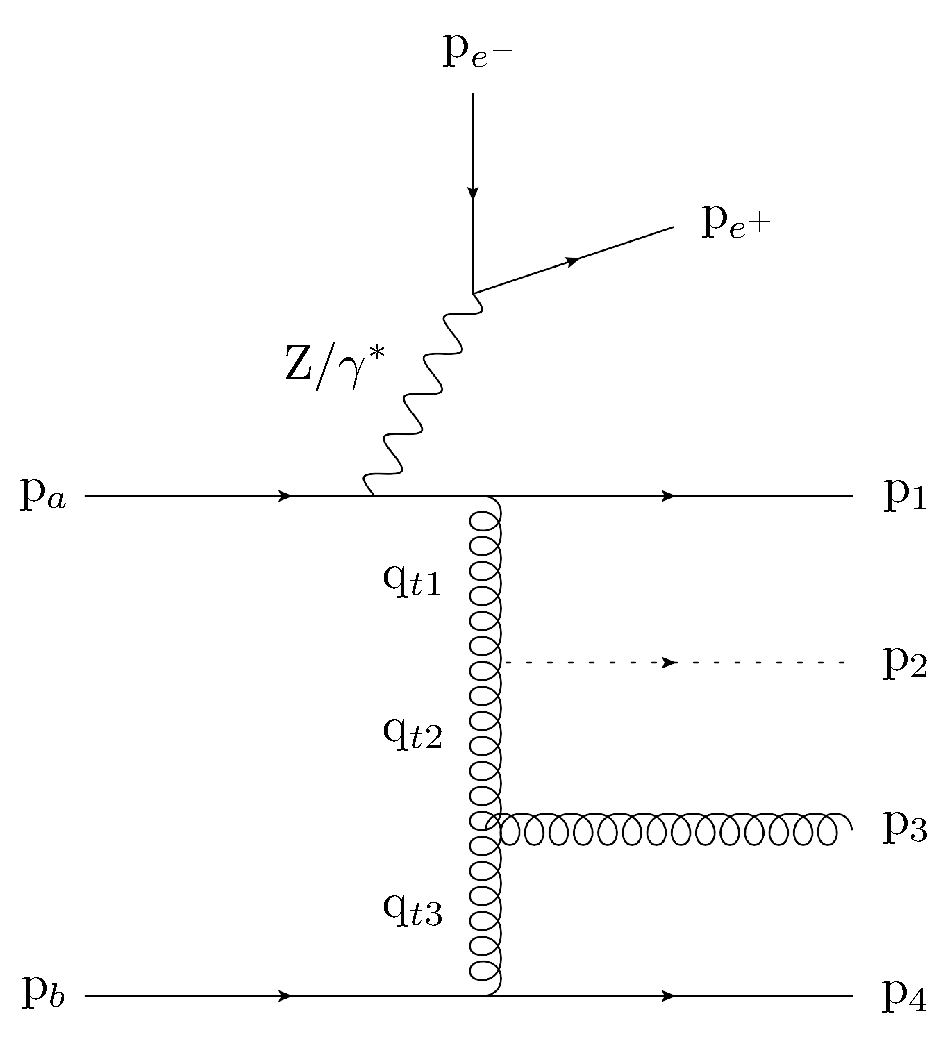
\includegraphics[width=1.0\linewidth]{RealSoftEmissionZ.pdf}
				\caption{}
				\label{fig:real24}
			\end{subfigure}

			\begin{subfigure}[b]{0.5\textwidth}
				\centering
				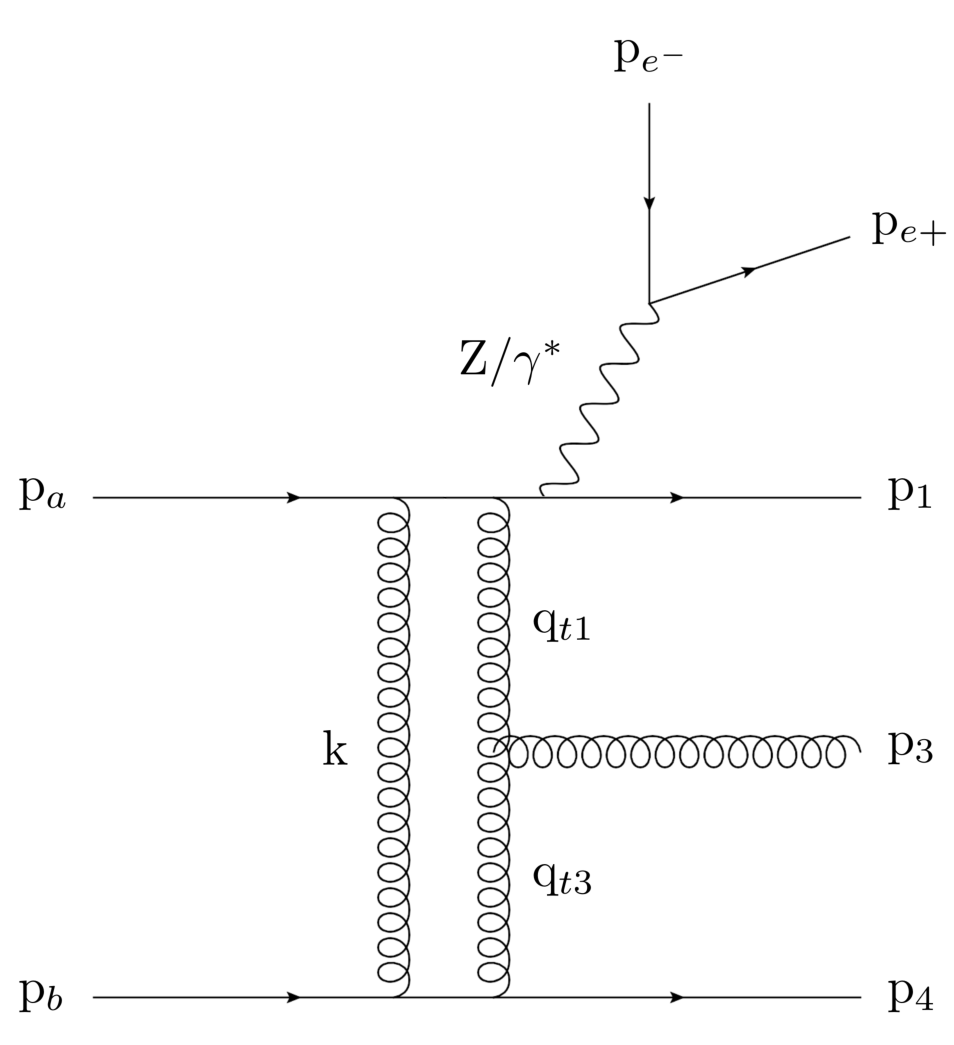
\includegraphics[width=1.0\linewidth]{VirtualSoftEmissionZ.pdf}
				\caption{}
				\label{fig:virtual23}
			\end{subfigure}

			\caption{Examples of both real and virtual diagrams contributing to
			$2\rightarrow3$ scattering. In fig. \eqref{fig:real24} the $p_2$ has been
			drawn with a dashed line to denote it is not resolvable.  In fig.
			\eqref{fig:virtual23} the final state momenta have been labelled in a
			seemingly strange way - this was done to make clear the cancellation
			when working through the algebra.}
			\label{fig:2to}
		\end{figure}

		Consider the case of $2\rightarrow3$ where the $p_2$ momentum has become soft.  A contributing
		soft diagram is shown in fig. \eqref{fig:real24} and one example of a contributing virtual
		diagram of the same order is shown in fig. \eqref{fig:virtual23}. When $p_2$ goes soft we have
		the following form for the $2\rightarrow3$ integrated amplitude squared ({N.B.}: The
		integration is only schematic and doesn't represent the full Lorentz invariant phase space):

		\begin{align}
		\begin{split}
			\int dPS|\mathcal{A}^{2\rightarrow3}_{soft}|^2 = &\frac{4C_Ag_s^2\Delta_{1,3}}{(2\pi)^{2+2\epsilon}4\pi}
			\frac{\pi^{\epsilon+1}}{\epsilon\Gamma(\epsilon+1)}
			\left(\frac{\lambda_{cut}^2}{\mu^2}\right)^\epsilon\Bigg[|\mathcal{K}_aj_1^Z\cdot j_2|^2
			\frac{V^2(q_{t1}, q_{t3})}{q^2_{t1}q^2_{t3}} \\
			+ |\mathcal{K}_bj_1\cdot j_2^Z|^2
			\frac{V^2(q_{b1}, q_{b3})}{q^2_{b1}q^2_{b3}} +
			& 2\Re\left\{\mathcal{K}_a\overline{\mathcal{K}_b}
			(j_1^Z\cdot j_2)\overline{(j_1\cdot j_2^Z)}\right\} \frac{V(q_{t1}, q_{t3})
			\cdot V(q_{b1}, q_{b3})}{q_{t1}q_{t3}q_{b1}q_{b3}}\Bigg],
		\end{split}
		\end{align}

		and the virtual contributions for the $2\rightarrow3$ amplitude is:

		\begin{align}
		\begin{split}
			\int dPS|\mathcal{A}^{2\rightarrow3}_{virtual}|^2 = &|\mathcal{K}_bj_1\cdot j_2^Z|^2
			\frac{V^2(q_{t1}, q_{t3})}{q_{t1}^2}e^{2\hat{\alpha}(q_{t1})\Delta_{1,3}} +
			|\mathcal{K}_tj_1^Z\cdot j_2|^2 \frac{V^2(q_{b1}, q_{b3})}{q_{b1}^2}e^{2\hat{\alpha}(q_{b1})\Delta_{1,3}} +  \\
			& 2\Re\left\{\mathcal{K}_a\overline{\mathcal{K}_b}  (j_1^Z\cdot j_2)\overline{(j_1\cdot j_2^Z)}\right\}
			\frac{V(q_{t1}, q_{t3})\cdot V(q_{b1}, q_{b3})}{q_{t1}q_{t3}q_{b1}q_{b3}}e^{(\hat{\alpha}(q_{t1}) +
			\hat{\alpha}(q_{b1}))\Delta_{1,3}}.
		\end{split}
		\end{align}

		Once we expand the exponential to the correct order in $g_s^2$, the sum of these
		matrix elements squared over the region of phase space when $p_2$ is soft is:

		\begin{align}
		\begin{split}
			\int dPS\left(|\mathcal{A}^{2\rightarrow3}_{soft}|^2 + |\mathcal{A}^{2\rightarrow3}_{virtual}|^2\right) =
			&|\mathcal{K}_aj_1^Z\cdot j_2|^2 \frac{V^2(q_{t1}, q_{t3})}{q_{t1}^2}
			{\Bigg(\frac{4C_Ag_s^2\Delta_{1,3}}{(2\pi)^{2+2\epsilon}4\pi}\frac{\pi^{\epsilon+1}}
			{\epsilon\Gamma(\epsilon+1)} - 2\hat{\alpha}(q_{t1})\Delta_{1,3}\Bigg)} + \\
			& |\mathcal{K}_bj_1\cdot j_2^Z|^2 \frac{V^2(q_{b1}, q_{b3})}{q_{b1}^2}
			{\Bigg(\frac{4C_Ag_s^2\Delta_{1,3}}{(2\pi)^{2+2\epsilon}4\pi}\frac{\pi^{\epsilon+1}}
			{\epsilon\Gamma(\epsilon+1)} - 2\hat{\alpha}(q_{b1})\Delta_{1,3}\Bigg)}+ \\
			&2\Re\left\{\mathcal{K}_a\overline{\mathcal{K}_b}  (j_1^Z\cdot j_2)\overline{(j_1\cdot j_2^Z)}\right\}
			\frac{V(q_{t1}, q_{t3})\cdot V(q_{b1}, q_{b3})}{q_{t1}q_{t3}q_{b1}q_{b3}}\\
			&{\Bigg(\frac{4C_Ag_s^2\Delta_{1,3}}{(2\pi)^{2+2\epsilon}4\pi}\frac{\pi^{\epsilon+1}}{\epsilon\Gamma(\epsilon+1)} -
			(\hat{\alpha}(q_{t1}) + \hat{\alpha}(q_{b1}))\Delta_{1,3}\Bigg)} + \mathcal{O}(g_s^4),
		\end{split}
		\end{align}

		These bracketed terms are exactly the cancellations calculated in section 4 above.  Therefore:

		\begin{align}
		\begin{split}
			\int dPS\left(|\mathcal{A}^{2\rightarrow3}_{soft}|^2 + |\mathcal{A}^{2\rightarrow3}_{virtual}|^2\right) =&
			\frac{\alpha_sC_A\Delta_{1,3}}{\pi}\Bigg(|\mathcal{K}_aj_1^Z\cdot j_2|^2 \frac{V^2(q_{t1},
			q_{t3})}{q_{t1}^2}\ln\left(\frac{\lambda_{cut}^2}{|q_{1t\perp}|^2}\right)+ \\
			& |\mathcal{K}_bj_1\cdot j_2^Z|^2 \frac{V^2(q_{b1}, q_{b3})}{q_{b1}^2}\ln
			\left(\frac{\lambda_{cut}^2}{|q_{1b\perp}|^2}\right)+ \\
			&2\Re\left\{\mathcal{K}_a\overline{\mathcal{K}_b}  (j_1^Z\cdot j_2)\overline{(j_1\cdot j_2^Z)}\right\}
			\frac{V(q_{t1}, q_{t3})\cdot V(q_{b1}, q_{b3})}{q_{t1}q_{t3}q_{b1}q_{b3}}\\
			&\ln\left(\frac{\lambda_{cut}^2}{\sqrt{|q_{1t\perp}|^2|q_{1b\perp}|^2}}\right)\Bigg) + \mathcal{O}(\alpha_s^2),
		\end{split}
		\end{align}

		Which is manifestly finite.

\section{Subtractions and the $\lambda_{cut}$ scale}
	\label{sec:indep-lambd}

	We now show the stability of the High Energy Jets predictions with respect to the
	$\lambda_{cut}$ scale described above.\\We
	increase our sensitivity to the parameter by showing results for FKL momentum
	configurations only.  The non-FKL samples which are added to give the total
	cross sections have no dependence on $\lambda_{cut}$ and would therefore dilute
	any dependence in the full sample.  We begin in table~\ref{tab:lambdaxs} where we show the value of
	the cross section for different values of $\lambda_{cut}$ for exclusive 2-, 3-
	and 4-jet samples.  The cuts applied are the same as in section \ref{sub:ATLAS}.
	It is clear that the cross section does not display a large dependence on the
	value of $\lambda_{cut}$.

	\begin{table}[htp!]
		\begin{center}
		\begin{tabular}{| c | c | c | c |}
		\hline
		$\lambda_{cut}$ (GeV) & $\sigma(2j)$ ($pb$) & $\sigma(3j)$ ($pb$) & $\sigma(4j)$ ($pb$) \\ \hline
		0.2 & $5.03 \pm 0.02$ & $0.70 \pm 0.02$ & $0.13 \pm 0.03$ \\
		0.5 & $5.05 \pm 0.01$ & $0.70 \pm 0.01$ & $0.13 \pm 0.01$ \\
		1.0 & $5.09 \pm 0.01$ & $0.71 \pm 0.01$ & $0.13 \pm 0.01$ \\
		2.0 & $5.16 \pm 0.04$ & $0.72 \pm 0.01$ & $0.13 \pm 0.01$ \\ \hline
		\end{tabular}
		\caption{The FKL-only cross sections for the 2-, 3- and 4-jet exclusive rates
		with associated statistical errors shown for different values of the regularisation parameter
		$\lambda_{cut}$.  The scale choice was half the sum over all transverse scales in the event, $H_T/2$.}
		\label{tab:lambdaxs}
		\end{center}
	\end{table}

	Figure~\ref{fig:lambdadist} shows the effect of the same variation in $\lambda_{cut}$ on the
	differential distribution in both the rapidity gap between the two leading jets in $p_\perp$,
	$\Delta y_{j1, j2}$, (a)--(c), and the rapidity gap between the two extremal jets in
	rapidity, $\Delta y_{jf, jb}$, (d)--(f).  Results are shown for exclusive 2-, 3-
	and 4-jet samples in each case, once again the cuts applied are the same as in the ATLAS study
	presented in section \ref{sub:ATLASZsec}.
	Again the scale choice for the central line was $\mu_F=\mu_R=H_T/2$.  The variation bands
	have been determined by varying these two scales independently by up to a factor of two
	in either direction with the extremal points removed where the relative difference between
	$\mu_F$ and $\mu_R$ is greater than a factor of 2.  The distributions also show a very weak
	dependence on the choice of $\lambda_{cut}$.

	In practice, our default chosen value for $\lambda_{cut}$ is 0.2.

	\begin{figure}[htp!]
		\centering
		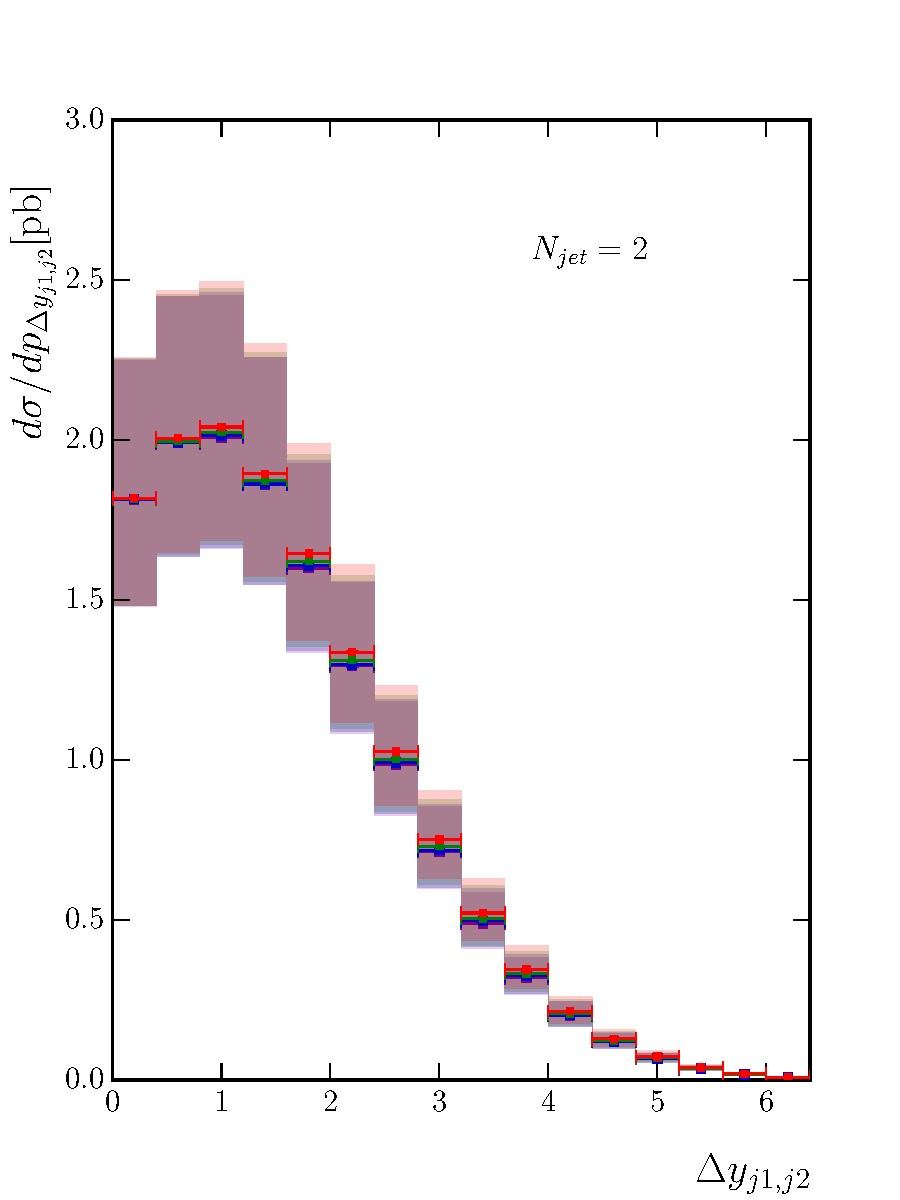
\includegraphics[width=.5\textwidth]{Z_11a_2j.pdf}\hfill
		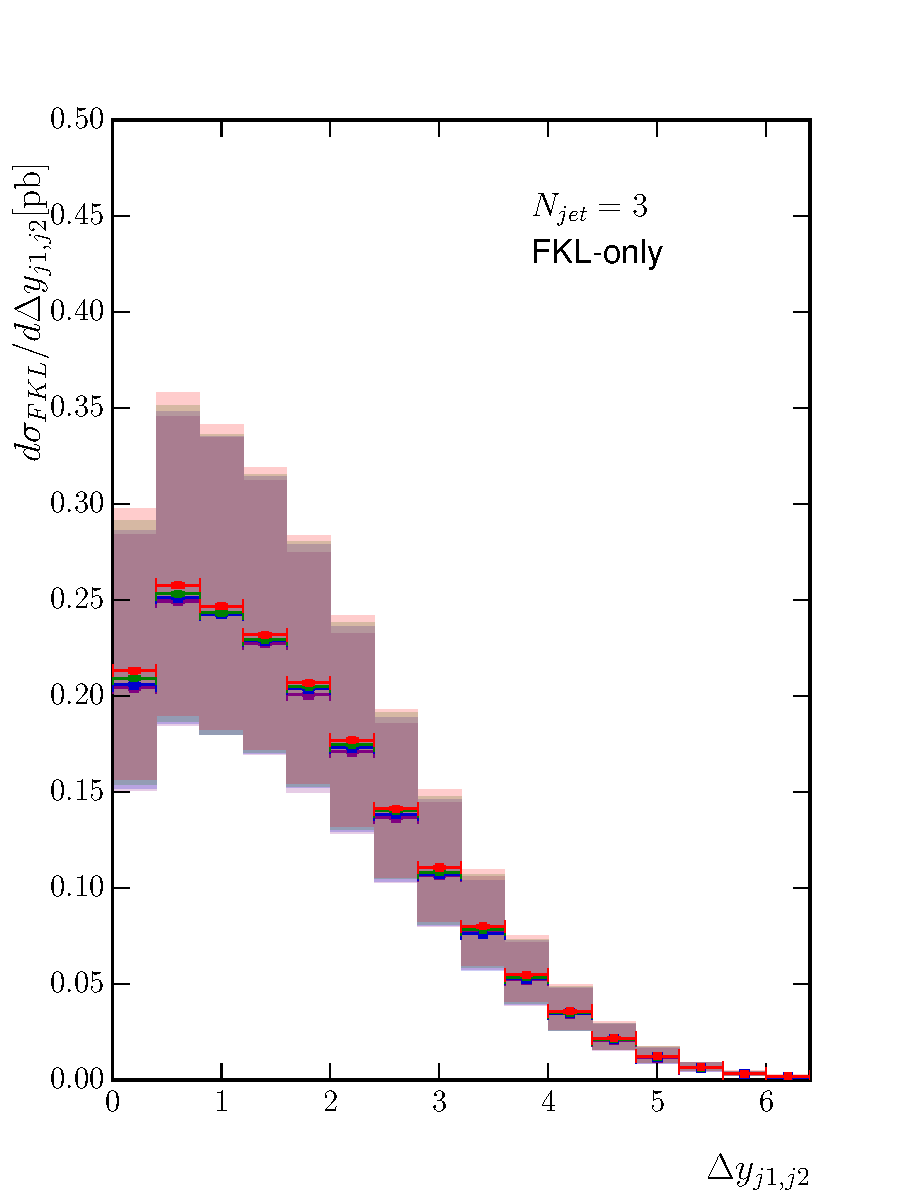
\includegraphics[width=.5\textwidth]{Z_11a_3j.pdf}\hfill
		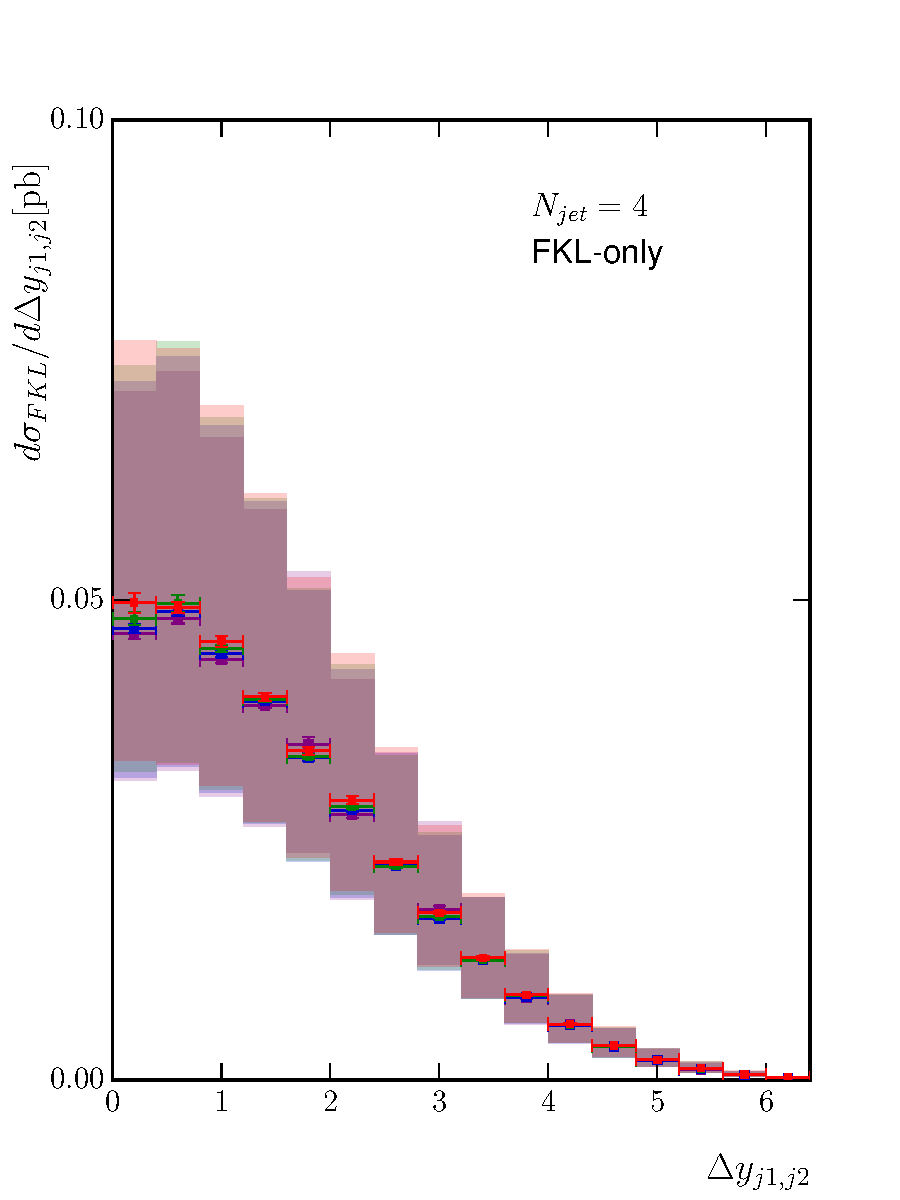
\includegraphics[width=.5\textwidth]{Z_11a_4j.pdf}
		\caption{The effect of varying $\lambda_{cut}$ on the differential distribution
		in the rapidity gap between the two leading jets in $p_\perp$, $\Delta y_{j1, j2}$,
		with the $N_{jet}=2,3,4$ exclusive selections shown from left to right.
		$\lambda_{cut}=0.2$ (red), 0.5 (blue), 1.0 (green), 2.0 (purple).
		The bands represent the scale variation described in the text.}
		\label{fig:lambdadist}
	\end{figure}

	\begin{figure}[htp!]
		\centering
		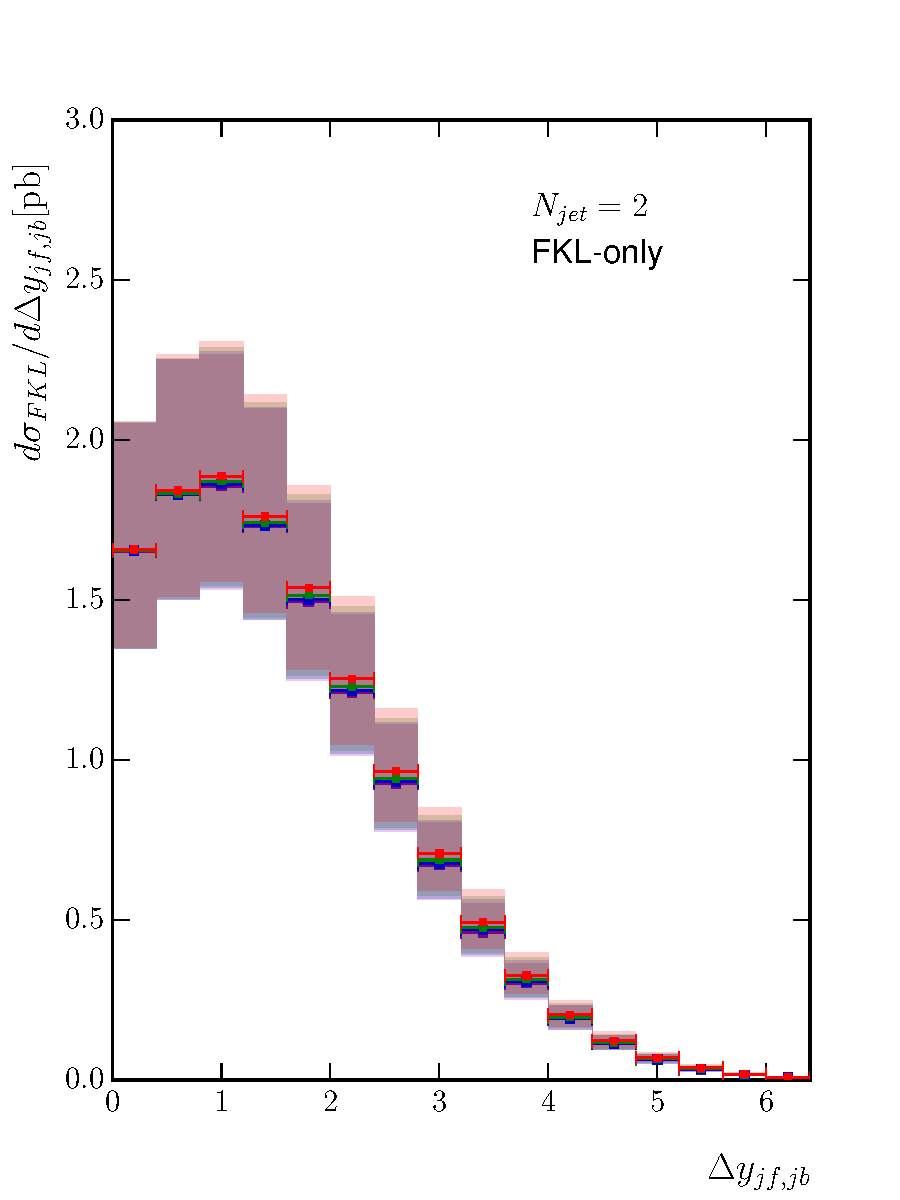
\includegraphics[width=.5\textwidth]{Z_11c_2j.pdf}\hfill
		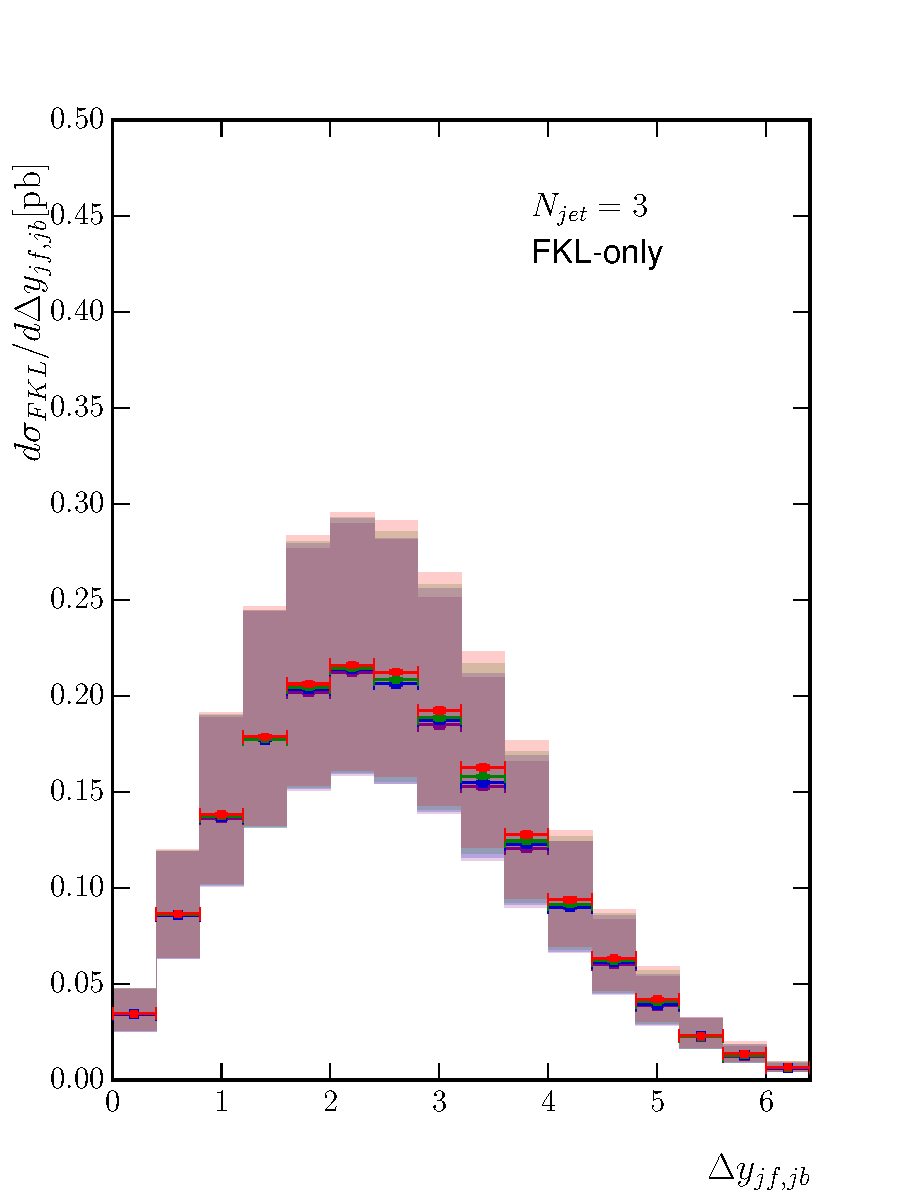
\includegraphics[width=.5\textwidth]{Z_11c_3j.pdf}\hfill
		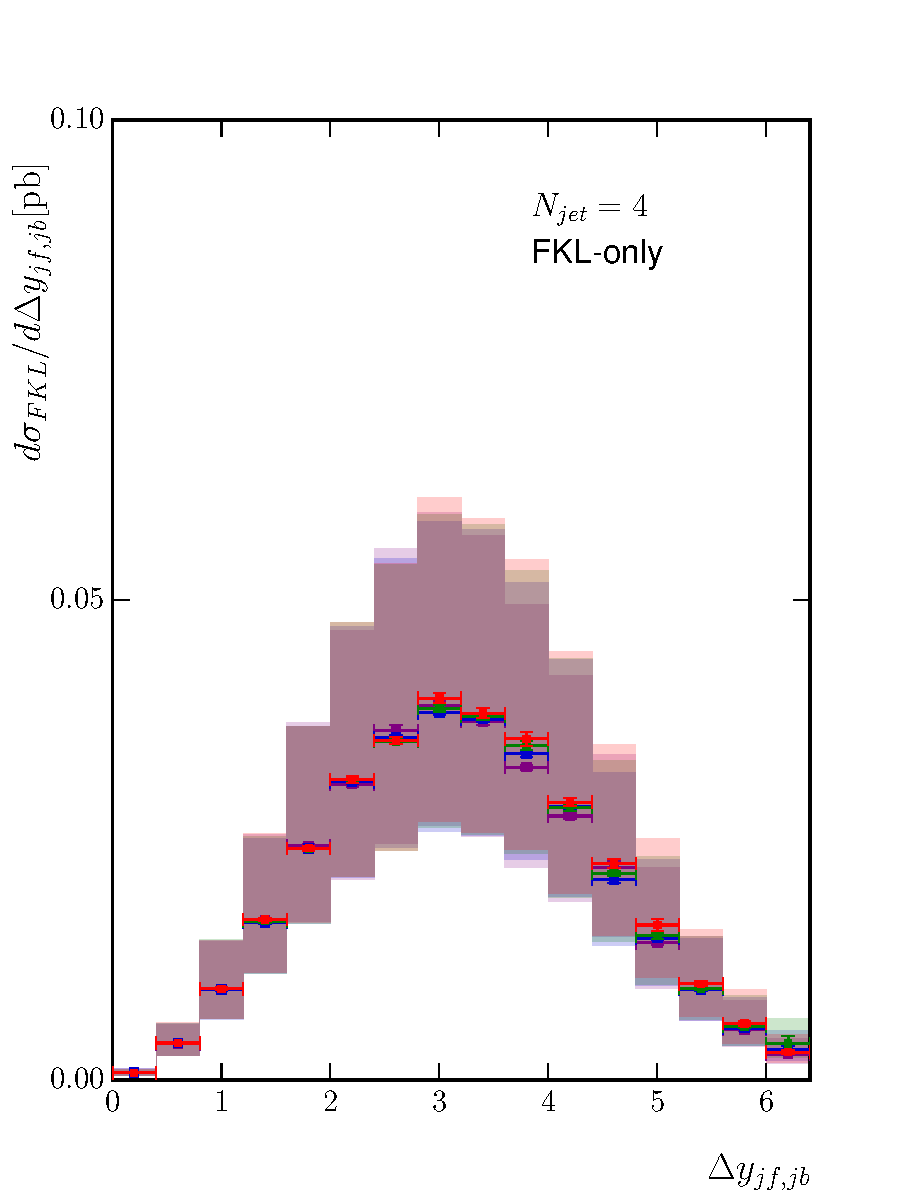
\includegraphics[width=.5\textwidth]{Z_11c_4j.pdf}
		\caption{The effect of varying $\lambda_{cut}$ on the differential distribution
		in the rapidity gap between the two extremal jets in rapidity, $\Delta y_{jf, jb}$,
		with the $N_{jet}=2,3,4$ exclusive selections shown from left to right.
		$\lambda_{cut}=0.2$ (red), 0.5 (blue), 1.0 (green), 2.0 (purple).
		The bands represent the scale variation described in the text.}
		\label{fig:lambdadistdy}
	\end{figure}

\section{The Differential ${Z/\gamma}$ Cross-Section}

	Starting from eqn. \eqref{eq:allordereg} we can write down a total (differential)
	cross section can then be obtained by summing over all values of $n$ and
	integrating over the full $n$-particle phase space, using an efficient Monte
	Carlo sampling algorithm~\cite{Andersen:2008ue,Andersen:2008gc}:

	\begin{align}
	  \label{eq:sigma}
	  \begin{split}
	    \sigma =& \sum_{f_a,f_b} \sum_{n=2}^\infty \int \frac{d^3 p_a}{(2\pi)^3 2E_a} \int \frac{d^3
	      p_b}{(2\pi)^3 2E_b}  \left( \prod_{i=2}^n \int \frac{d^3 p_i}{(2\pi)^3
	        2E_i} \right)\ (2\pi)^4 \delta^{(4)}\left(p_a+p_b - \sum_i p_i\right) \\
	    & \ \times \ |\mathcal{M}^{HEJ-{\rm reg}}_{f_af_b\to \zg
	      f_a(n-2)gf_b}(p_a,p_b,\{p_i\})|^2 \ \frac{ x_a f_{f_a}(x_a, Q_a) x_b
	      f_{f_b}(x_b,Q_b)}{\hat s^2}\ \Theta_{\rm cut},
	  \end{split}
	\end{align}

	where $x_{a,b}$ are the momentum fractions of the incoming partons and
	$f_{f_k}(x_k,Q_k)$ are the corresponding parton density functions for beam,
	k, and flavour $f_k$.  The factor of $\hat s^2$ is the usual phase space
	factor.  The function $\Theta_{\rm cut}$ term imposes any desired cuts on the final
	state.  The minimum requirement is that the final state momenta cluster into at
	least two jets for the desired algorithm

	In the regions of phase space where all final state particles are well separated
	in rapidity, this gives the dominant terms in QCD at all orders in $\alpha_s$  (the leading logarithmic
	terms in $s/t$).  However, in other areas of
	phase space, the differences due to the approximations used in
	$|\mathcal{M}^{HEJ-{\rm reg}}_{qQ\to \zg q(n-2)gQ}|^2$ will become more
	significant.  We can therefore further improve upon eq.~\eqref{eq:sigma} by
	matching our results to fixed order results.  Here, we match to
	high-multiplicity tree-level
	results obtained from \texttt{Madgraph5}~\cite{Alwall:2014hca} in two different ways.
	This amounts to merging tree-level samples of different orders according to the
	logarithmic prescription of HEJ.

	\begin{enumerate}
		\item Matching for FKL configurations
		  As described in section~\ref{sec:HEQCD}, these are the particle assignments
		  and momentum configurations which contain the dominant leading-logarithmic
		  terms in $s/t$.  The first step of the HEJ description was to develop an
		  approximation to the matrix element for these processes which was later
		  supplemented with the finite correction which remained after cancelling the
		  real and virtual divergences: $\overline{|\mathcal{M}_{qg\to Zqg}^{HE}|}^2$
		  (eq.~(\ref{eq:qgamp})) or $\overline{|\mathcal{M}_{qQ\to ZqQ}^{HE}|}^2$
		  (eq.~(\ref{eq:allorderreal})).  The approximation is necessary to allow us to
		  describe the matrix element for any (and in particular, large) $n$ and for
		  including both the leading real and virtual corrections.  However,
		  if the parton momenta cluster into four or fewer \emph{jets} (These
		  may have arisen from many more partons), the full tree-level matrix element remains
		  calculable.  In these cases, we perform the matching multiplicatively, so we
		  multiply the integrand of eq.~(\ref{eq:sigma}) by

		  \begin{align}
		    |\mathcal{M}^{\rm full}_{qQ\to \zg q(k-2)gQ}(p_a,p_b,\{
		    j_i'\})|^2/|\mathcal{M}^{HEJ}_{qQ\to \zg q(k-2)gQ}(p_a,p_b,\{j_i'\})|^2.
		  \end{align}

		  Here, $\{j_i'\}$ are the jet momenta after a small amount of
		  reshuffling.  This is necessary because the evaluation of the tree-level matrix elements
		  assumes that the jet momenta are both on-shell and have transverse momenta which
		  sum to zero, neither of which is true in general for our events due to the
		  presence of extra emissions.  Our reshuffling algorithm~\cite{Andersen:2011hs} redistributes this
		  extra transverse momentum in proportion to the size of the transverse
		  momentum of each jet.  The plus and minus light-cone components are then adjusted such
		  that the jet is put on-shell and the rapidity remains unaltered.  This last
		  feature ensures that after reshuffling the event is still in an FKL
		  configuration.

		  After this multiplicative matching factor has been included, the regularisation then proceeds as before.

		\item Matching for non-FKL configurations

		  Away from regions in phase space where the quarks and gluons are
		  well-separated, the non-FKL configurations will play a more significant
		  r\^ole.  These have so far not been accounted for at all, and hence we add
		  three exclusive samples of leading-order two-jet, three-jet and four-jet
		  leading-order events to our resummed events.  The distinction between the
		  samples is made following the choice of jet algorithm and parameters.

	\end{enumerate}

	These two matching schemes complete our description of the production of $\zg$
	with at least two jets, including the leading high-energy logarithms at all
	orders in $\alpha_s$.  In the next sections, we discuss the computational aspects
	of the work presented here and compare the resulting predictions from this formalism
	to LHC data from recent ATLAS and CMS analyses.

\section{$\zg$+Jets: Computational Aspects}

	The physics presented in the preceding sections is a significant departure from
	work previously done by the High Energy Jets collaboration.  As such developing
	the Monte Carlo for $\zg$ plus jets was a serious undertaking; the inclusion of
	the aforementioned interference terms required that two $t$-channel `chains' of
	momenta and vertices be computed.\\Furthermore to correctly calculate at the
	amplitude level the method in which we evaluate eqn. \ref{eq:Zcurrent}.  Since
	the virtual corrections are scale dependent it was necessary to change large
	sections of code to work with multiple copies of $t$-chains and multiple scales.\\
	The sections and chapters which follow contain theoretical predictions to
	experimental analyses.  These predictions were generated using distributed
	computing both locally in Edinburgh and using the CERN \texttt{GRID} system;
	the former required the development of a system to distributing, executing and
	finalising jobs across a large network of machines while the later involved
	learning who to interact with a computationally challenging system which was...
	{\color{red} a complete time-vampire and a real pain to use (rephrase this)}

\section{$\zg$+Jets at the LHC}

	\subsection{$\zg$+Jets at the ATLAS Experiment}
		\label{sub:ATLASZsec}

		We now compare the results of the formalism described in the previous sections
		to data.  We begin with a recent ATLAS analysis of $Z$-plus-jets events from
		7~TeV collisions~\cite{Aad:2013ysa}.  We summarise the cuts in the following
		table:

		\begin{table}[bth]
		  \centering
		  \begin{tabular}{|l|c|}
		    \hline
		    Lepton Cuts & $p_{T\ell}>20$~GeV, \; $|\eta_\ell|<2.5$ \\
		    & $\Delta R^{\ell^+\ell^-} > 0.2$, \; $66$~GeV $\leq m^{\ell^+\ell^-} \leq
		      116$~GeV \\ \hline
		    Jet Cuts (anti-$k_T$, 0.4) & $p_{Tj}>30$~GeV, \; $|y_j|<4.4$ \\
		    & $\Delta R^{j\ell} >0.5$ \\
		\hline
		  \end{tabular}
		  \caption{Cuts applied to theory simulations in the ATLAS
		    $Z$-plus-jets analysis results shown in Figs.~\eqref{fig:ATLAS_2a}--\eqref{fig:ATLAS_7b}.}
		  \label{tab:atlascuts}
		\end{table}

		Any jet which failed the final isolation cut was removed from the event, but the
		event itself is kept provided there are a sufficient number of other jets
		present.  Throughout the central value of the HEJ predictions has been
		calculated with factorisation and renormalisation scales set to
		$\mu_F=\mu_R=H_T/2$, and the theoretical uncertainty band has been determined by
		varying these independently by up to a factor of 2 in each direction (removing
		the corners where the relative ratio is greater than two).  Also shown in the
		plots taken from the ATLAS paper are theory predictions from
		Alpgen~\cite{Mangano:2002ea}, Sherpa~\cite{Gleisberg:2008ta,Hoeche:2012yf},
		MC@NLO~\cite{Frixione:2002ik} and
		BlackHat+Sherpa~\cite{Berger:2010vm,Ita:2011wn}.  We will also comment on the
		recent theory description of Ref.\cite{Frederix:2015eii} .

		In Fig.~\eqref{fig:ATLAS_2a}, we begin this set of comparisons with predictions
		and measurements of the inclusive jet rates.  HEJ and most of the other theory
		descriptions give a reasonable description of these rates.  The MC@NLO
		prediction drops below the data because it only contains the hard-scattering
		matrix element for $\zg$ production and relies on a parton shower for additional
		emissions. The HEJ predictions have a larger uncertainty band which largely
		arises from the use of leading-order results in the matching procedures.

		The first differential distribution we consider here is the distribution of the
		invariant mass between the two hardest jets, Fig.~\eqref{fig:ATLAS_11b}.  The
		region of large invariant mass is particularly important because this is a
		critical region for studies of vector boson fusion (VBF) processes in
		Higgs-plus-dijets.  Radiation patterns are largely universal between these
		processes, so one can test the quality of theoretical descriptions in
		$\zg$-plus-dijets and use these to inform the VBF analyses.  It is also a
		distribution which will be studied to try to detect subtle signs of new physics.
		In this study, HEJ and the other theory descriptions all give a good description
		of this variable out to 1~TeV, with HEJ being closest throughout the range.  The
		merged sample of Ref.~\cite{Frederix:2015eii} (Fig.~9 in that paper) combined
		with the Pythia8 parton shower performs reasonably well throughout the range
		with a few deviations of more than 20\%, while that combined with Herwig++
		deviates badly.  In a recent ATLAS analysis of $W$-plus-dijet
		events~\cite{Aad:2014qxa}, the equivalent distribution was extended out to 2~TeV
		and almost all of the theoretical predictions deviated significantly while the
		HEJ prediction remained flat.  This is one region where the high-energy
		logarithms which are only included in HEJ are expected to become large.

		In Fig.~\eqref{fig:ATLAS_11a}, we show the comparison of various theoretical
		predictions to the distribution of the absolute rapidity difference between the
		two leading jets.  It is clear in the left plot that HEJ gives an excellent
		description of this distribution.  This is to some extent expected as
		high-energy logarithms are associated with rapidity separations.  However, this
		variable is only the rapidity separation between the two hardest jets which is
		often not representative of the event as harder jets tend to be more central.
		Nonetheless, the HEJ description performs well in this restricted scenario.  The
		next-to-leading order (NLO) calculation of Blackhat+Sherpa also describes the
		distribution quite well while the other merged, fixed-order samples deviate from
		the data at larger values.  The merged samples of Ref.~\cite{Frederix:2015eii}
		(Fig.~8 in that paper) describe this distribution well for small values of this
		variable up to about 3 units when combined with Herwig++ and for most of the
		range when combined with the Pythia8 parton shower, only deviating above 5 units.

		The final distribution in this section is that of the ratio of the transverse
		momentum of the second hardest jet to the hardest jet.  The perturbative
		description of HEJ does not contain any systematic evolution of transverse
		momentum and this can be seen where its prediction undershoots the data at low
		values of $p_{T2}/p_{T1}$.  However, for values of $p_{T2} \gtrsim 0.5 p_{T1}$,
		the ratio of the HEJ prediction to data is extremely close to 1.  The
		fixed-order based predictions shown in Fig.~\eqref{fig:ATLAS_2a} are all fairly
		flat above about 0.2, but the ratio of the data differs by about 10\%.

		\newpage

		\begin{figure}[H]
		  \centering
		  \begin{subfigure}[b]{0.48\textwidth}
		    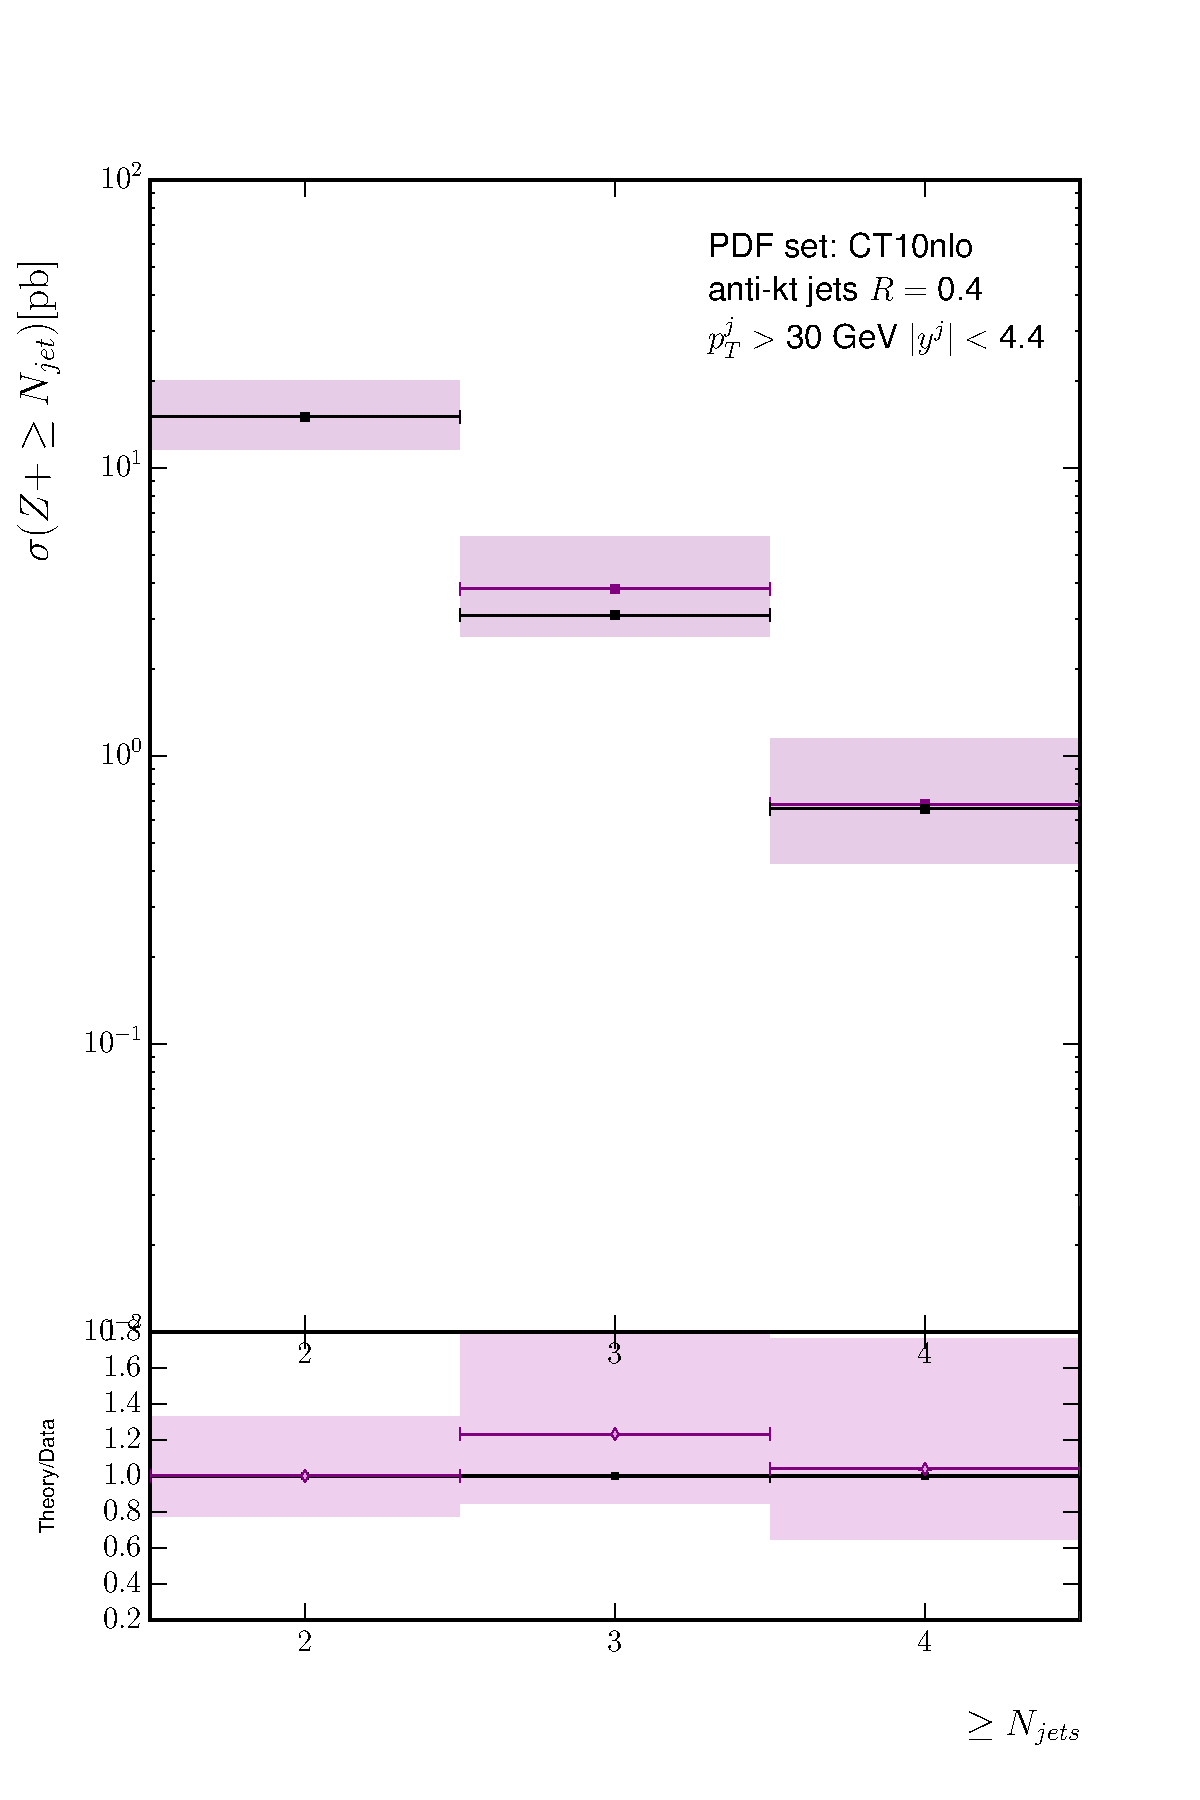
\includegraphics[width=\textwidth, height=1.2\textwidth]{ATLAS_Z_2a}
		    \label{fig:HEJ_ATLAS_2a}
		  \end{subfigure}
		  ~
		  \begin{subfigure}[b]{0.48\textwidth}
		    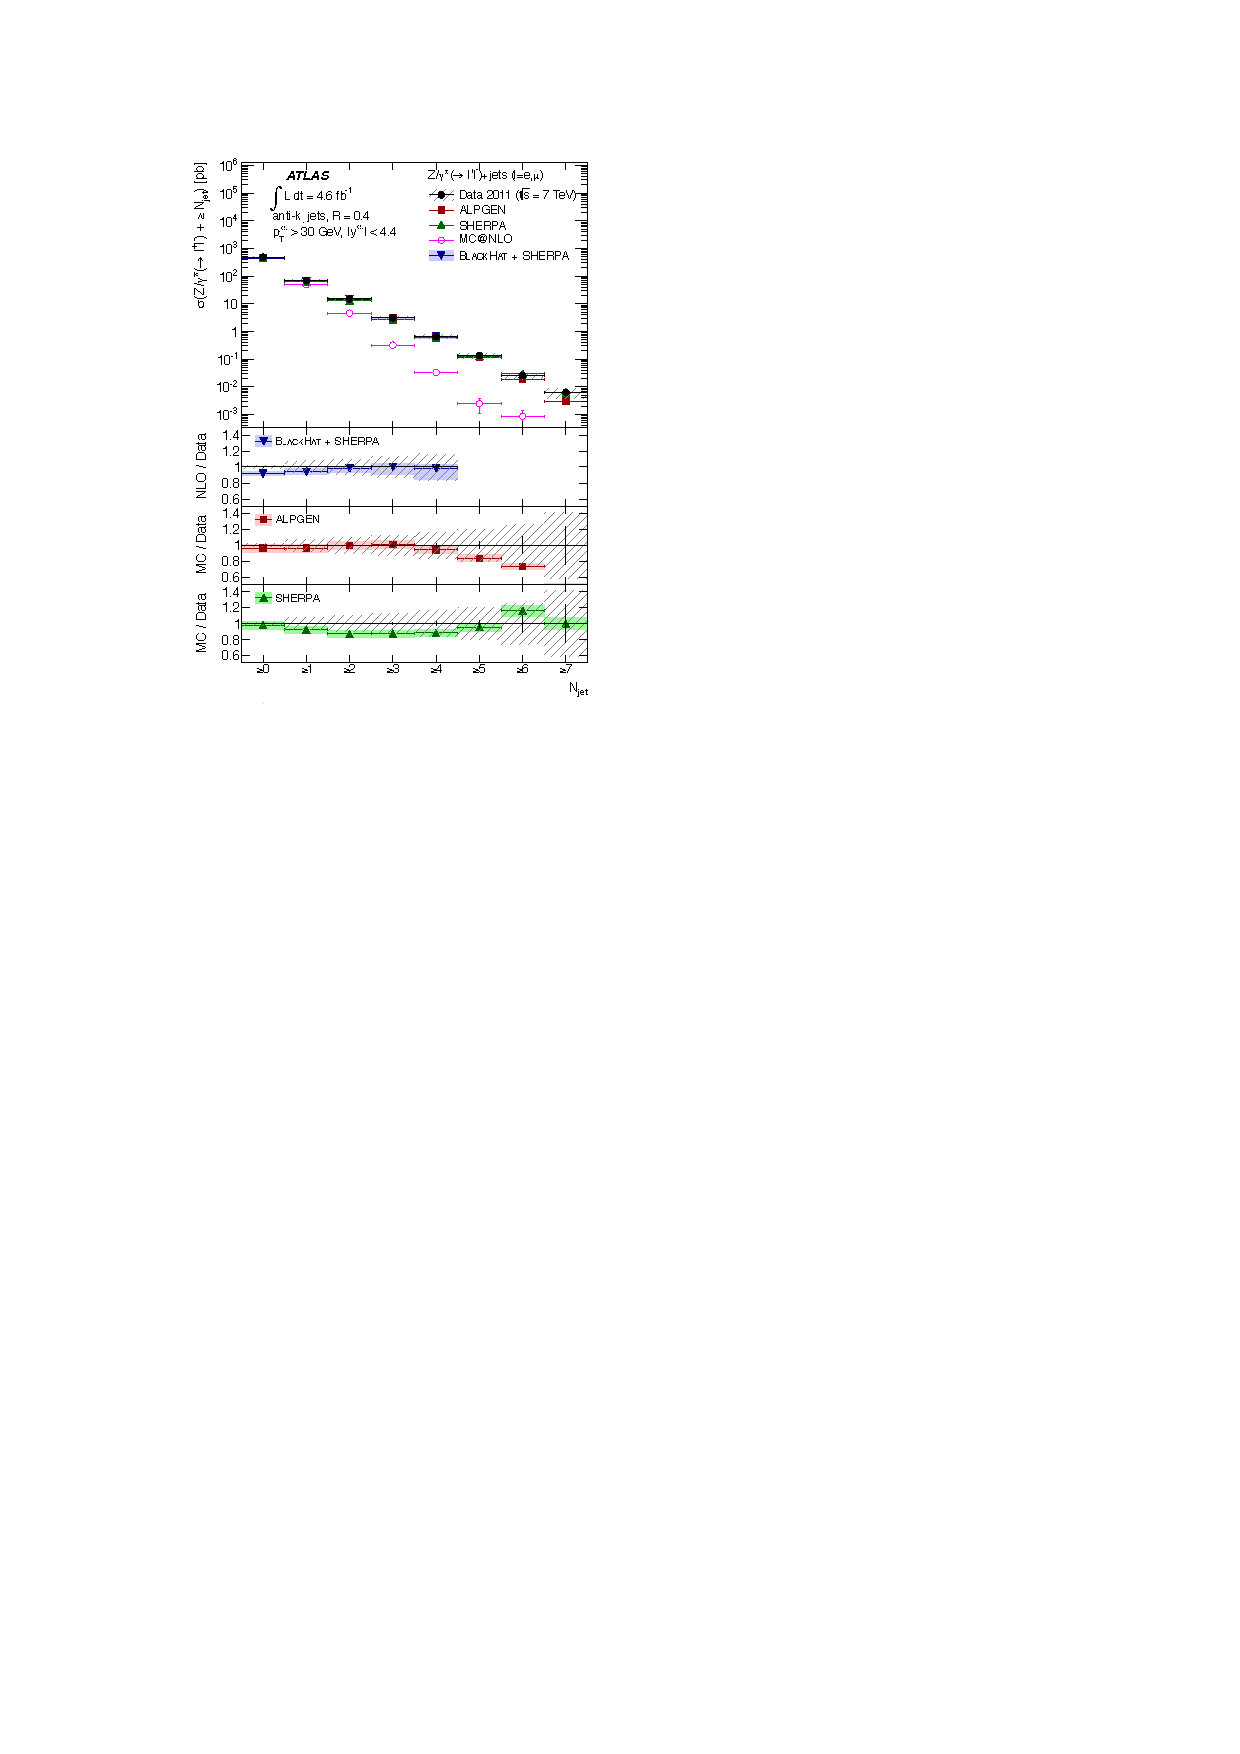
\includegraphics[width=\textwidth, height=1.2\textwidth]{Comparison_2a}
		    \caption{}
		    \label{fig:MC_ATLAS_2a}
		  \end{subfigure}
		  \caption{These plots show the inclusive jet rates from (a) HEJ and (b) other
		    theory descriptions and data~\cite{Aad:2013ysa}.  HEJ events all contain at
		    least two jets and do not contain matching for 5 jets and above, so these
		    bins are not shown.}
		  \label{fig:ATLAS_2a}

		  \begin{subfigure}[b]{0.48\textwidth}
		    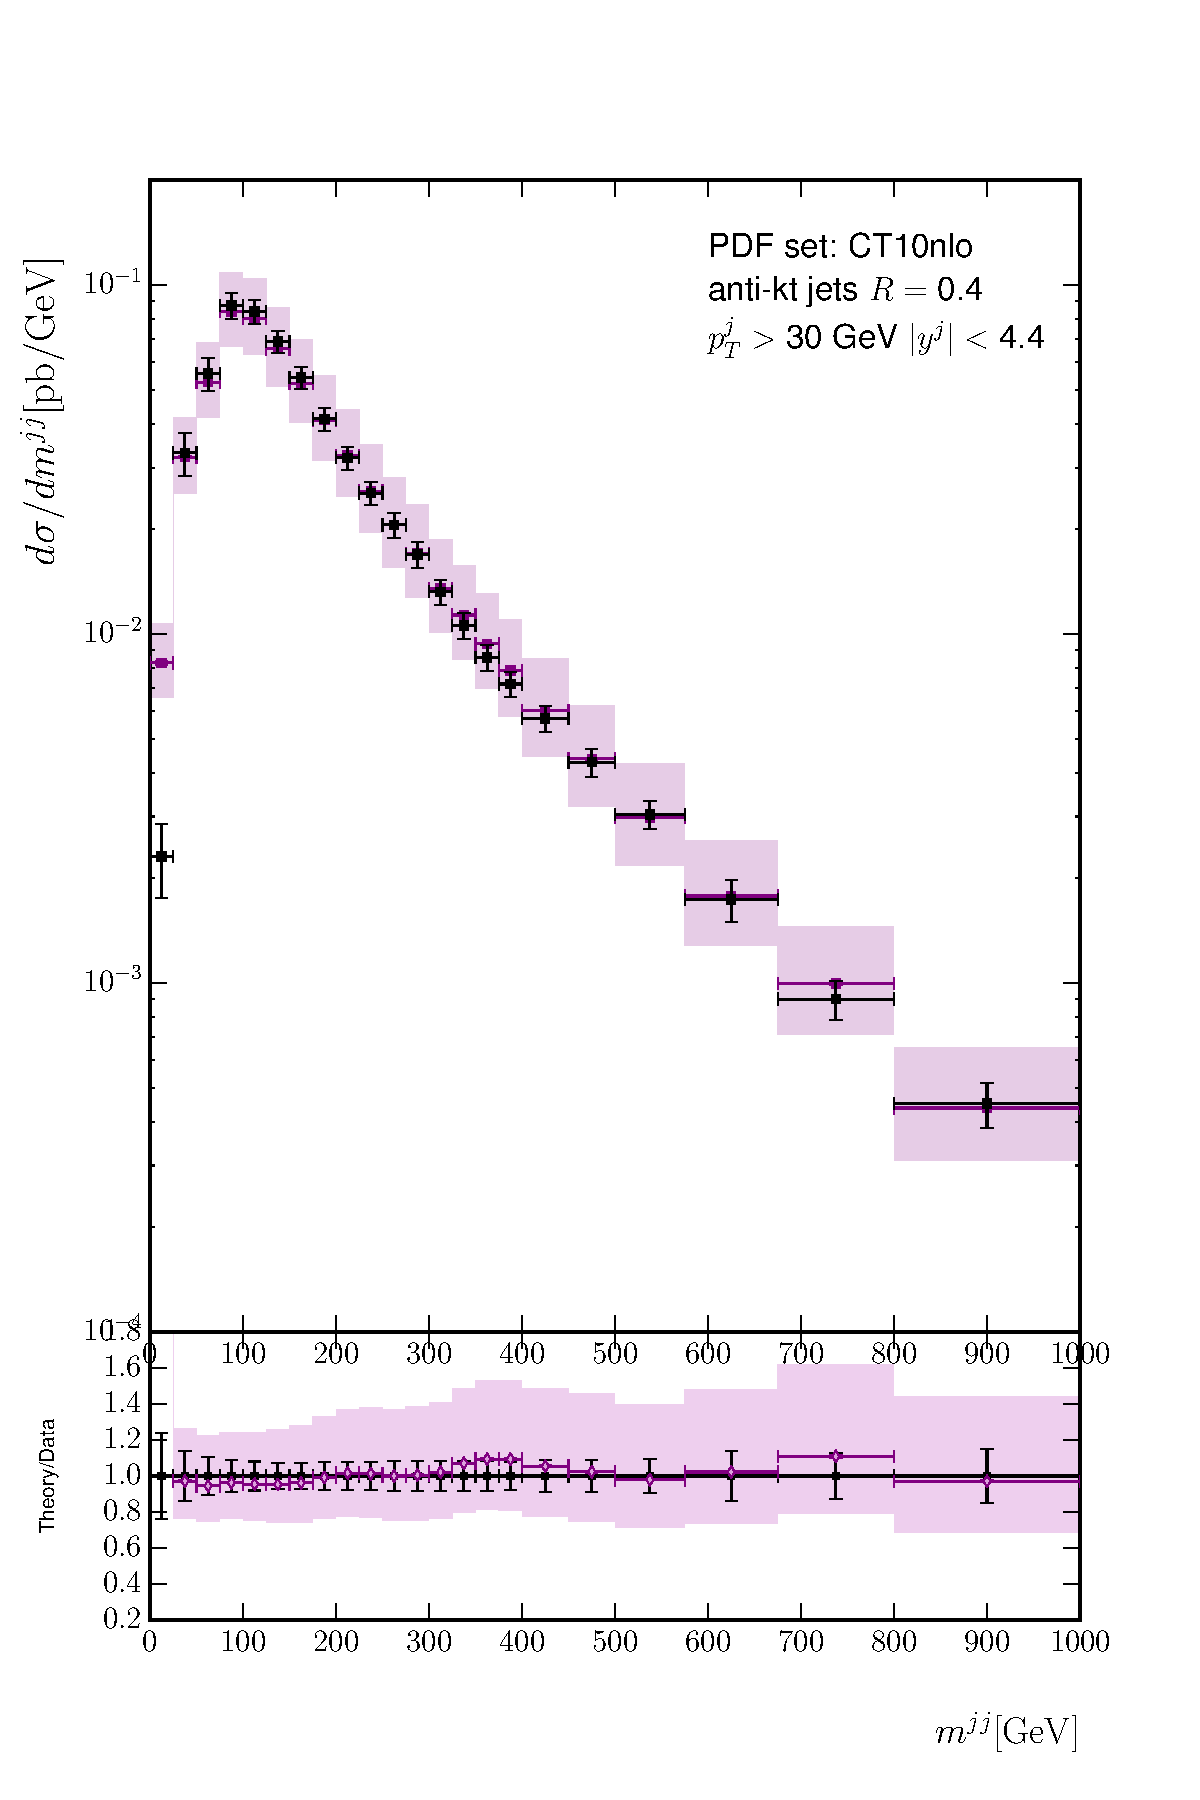
\includegraphics[width=\textwidth, height=1.2\textwidth]{ATLAS_Z_11b}
		    \caption{}
		    \label{fig:HEJ_ATLAS_11b}
		  \end{subfigure}
		  ~
		  \begin{subfigure}[b]{0.48\textwidth}
		    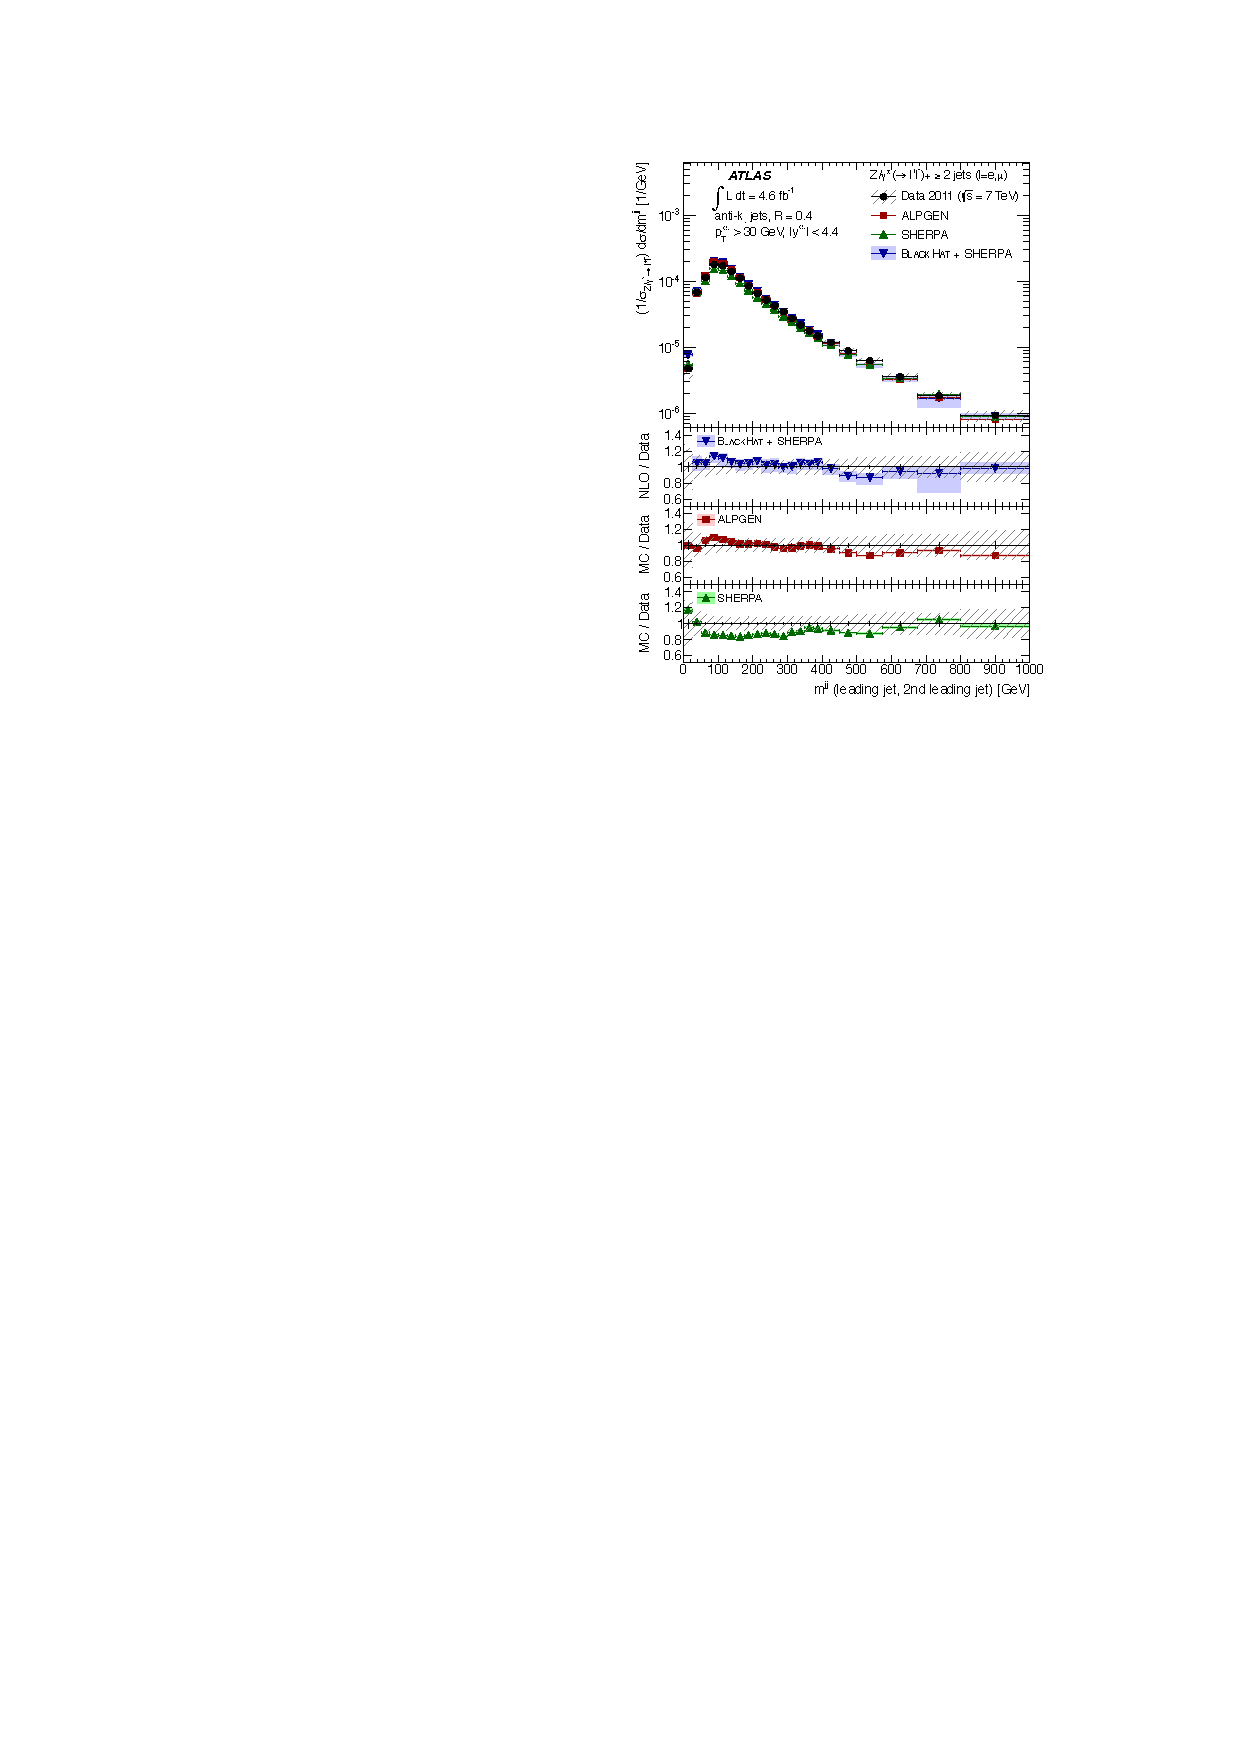
\includegraphics[width=\textwidth, height=1.2\textwidth]{Comparison_11b}
		    \caption{}
		    \label{fig:MC_ATLAS_11b}
		  \end{subfigure}
		  \caption{These plots show the invariant mass between the leading and
		    second-leading jet in $p_T$.  As in Fig.~\eqref{fig:ATLAS_2a}, predictions are
		    shown from (a) HEJ and (b) other theory descriptions and
		    data~\cite{Aad:2013ysa}. These studies will inform Higgs plus dijets
		    analyses, where cuts are usually applied to select events with large
		    $m_{12}$.}
		  \label{fig:ATLAS_11b}
		\end{figure}

		\begin{figure}[h]
		  \centering
		  \begin{subfigure}[b]{0.48\textwidth}
		    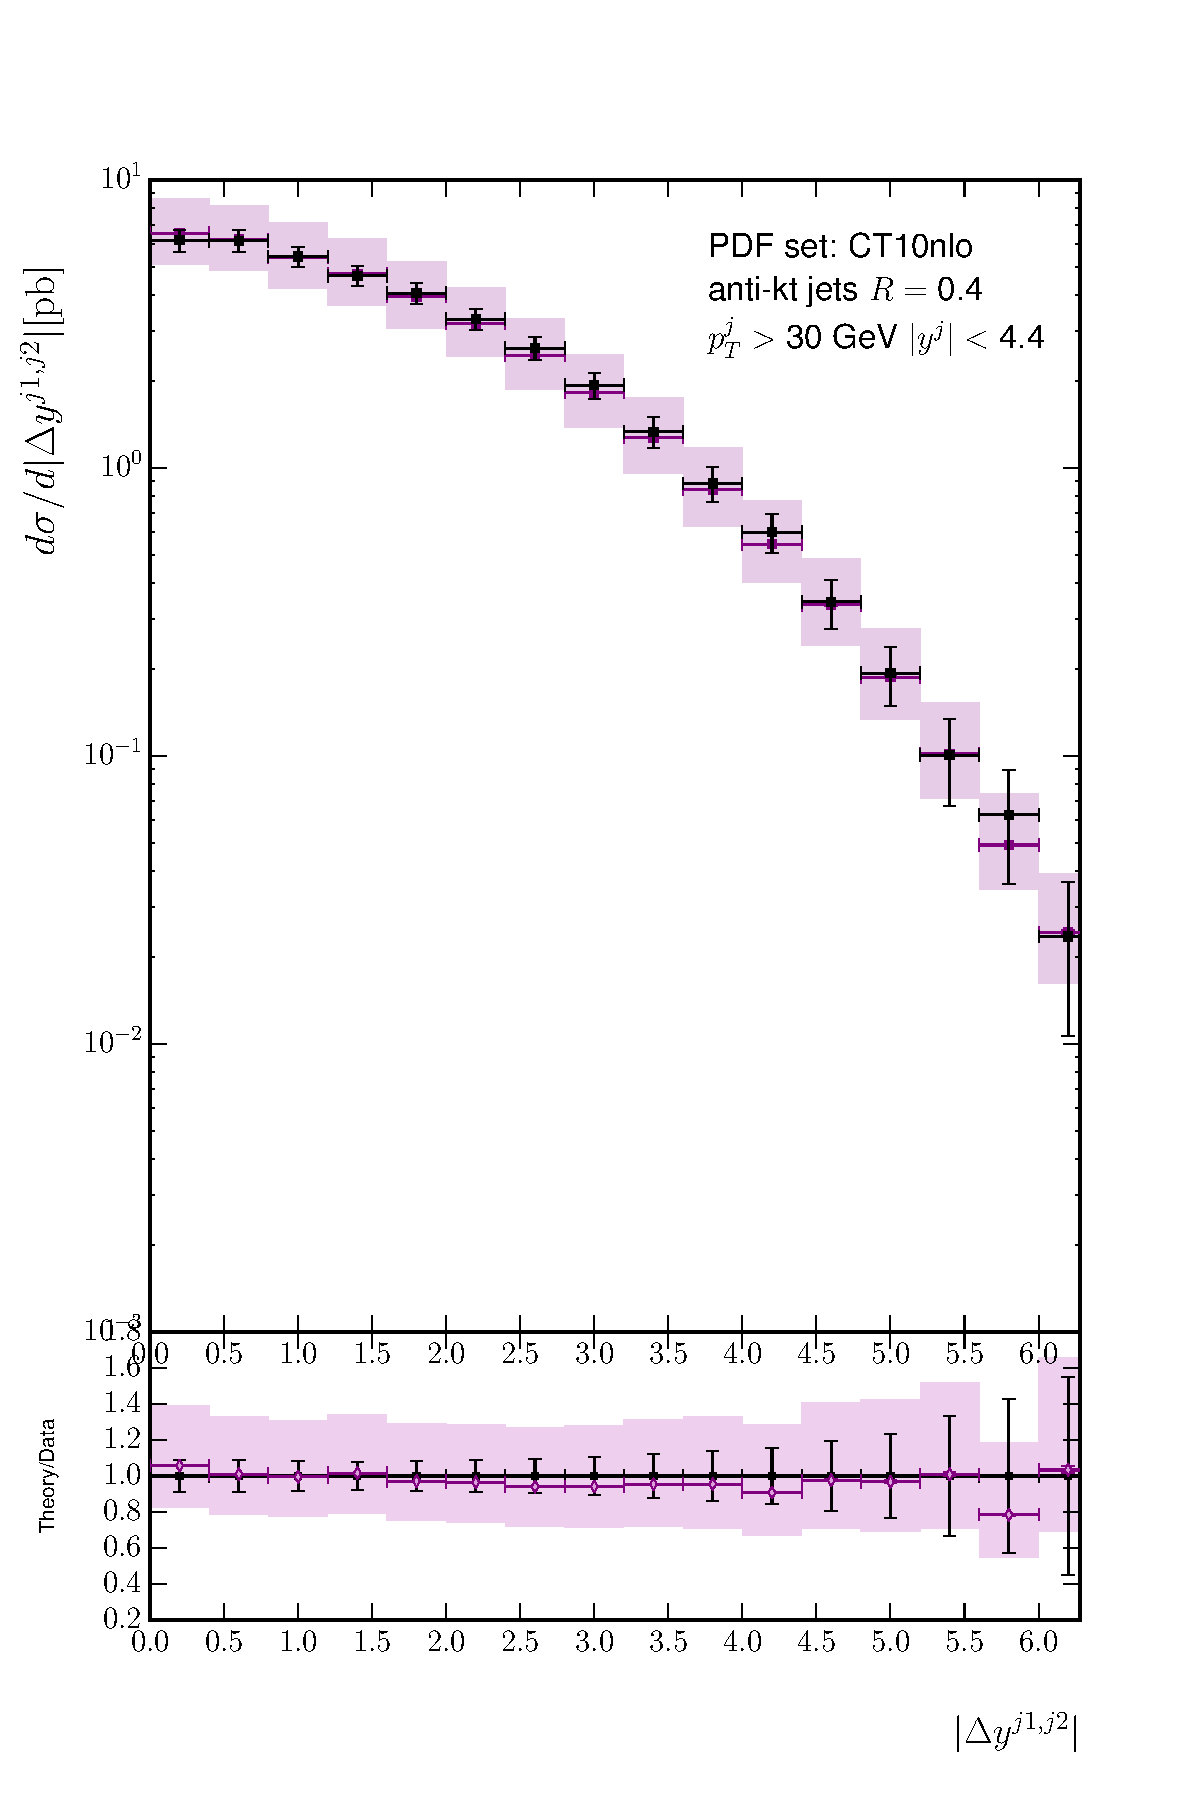
\includegraphics[width=\textwidth, height=1.2\textwidth]{ATLAS_Z_11a}
		    \caption{}
		    \label{fig:HEJ_ATLAS_11a}
		  \end{subfigure}
		  ~
		  \begin{subfigure}[b]{0.48\textwidth}
		    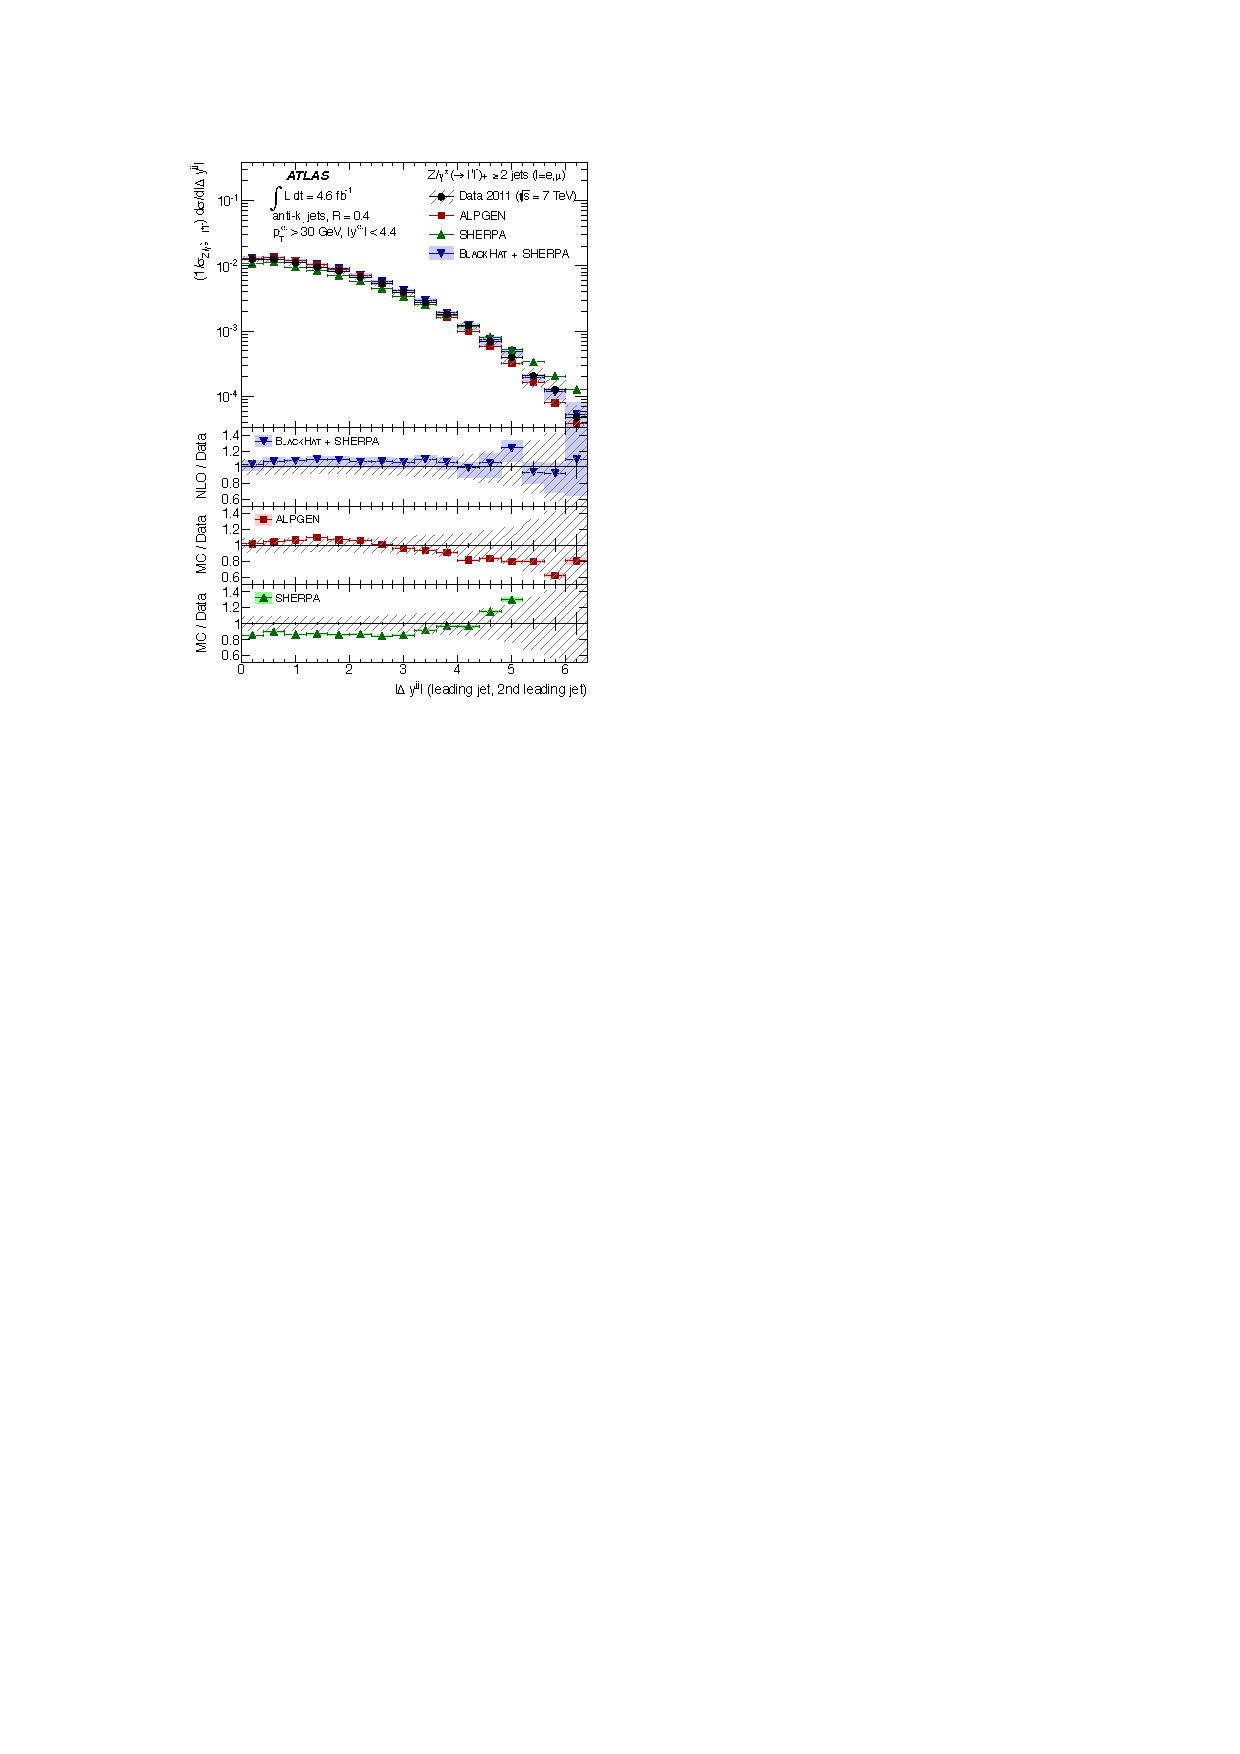
\includegraphics[width=\textwidth, height=1.2\textwidth]{Comparison_11a}
		    \caption{}
		    \label{fig:MC_ATLAS_11a}
		  \end{subfigure}
		  \caption{The comparison of (a) HEJ and (b) other theoretical descriptions and
		    data~\cite{Aad:2013ysa} to
		    the distribution of the absolute rapidity different between the two leading
		    jets.  HEJ and Blackhat+Sherpa give the best description.}
		  \label{fig:ATLAS_11a}

		  \begin{subfigure}[b]{0.48\textwidth}
		    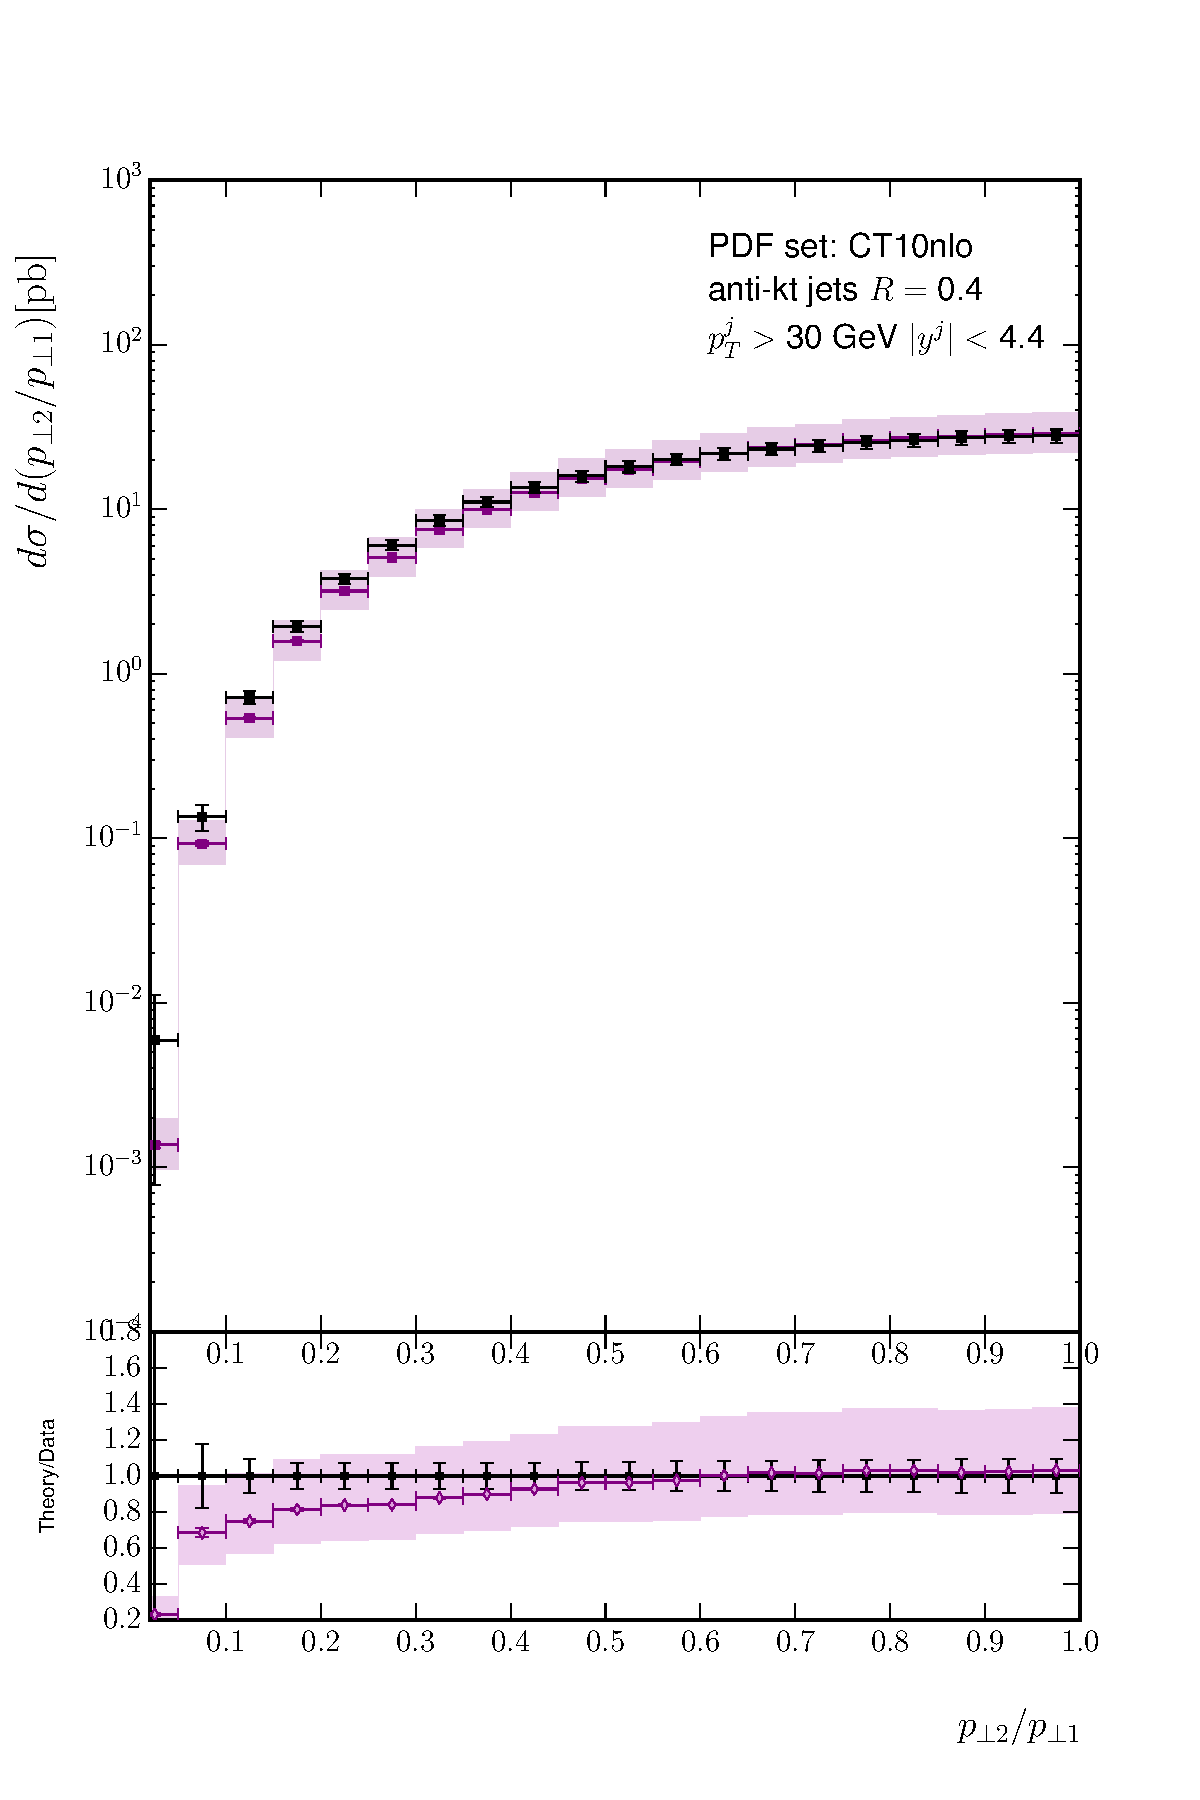
\includegraphics[width=\textwidth, height=1.2\textwidth]{ATLAS_Z_7b}
		    \caption{}
		    \label{fig:HEJ_ATLAS_7b}
		  \end{subfigure}
		  ~
		  \begin{subfigure}[b]{0.48\textwidth}
		    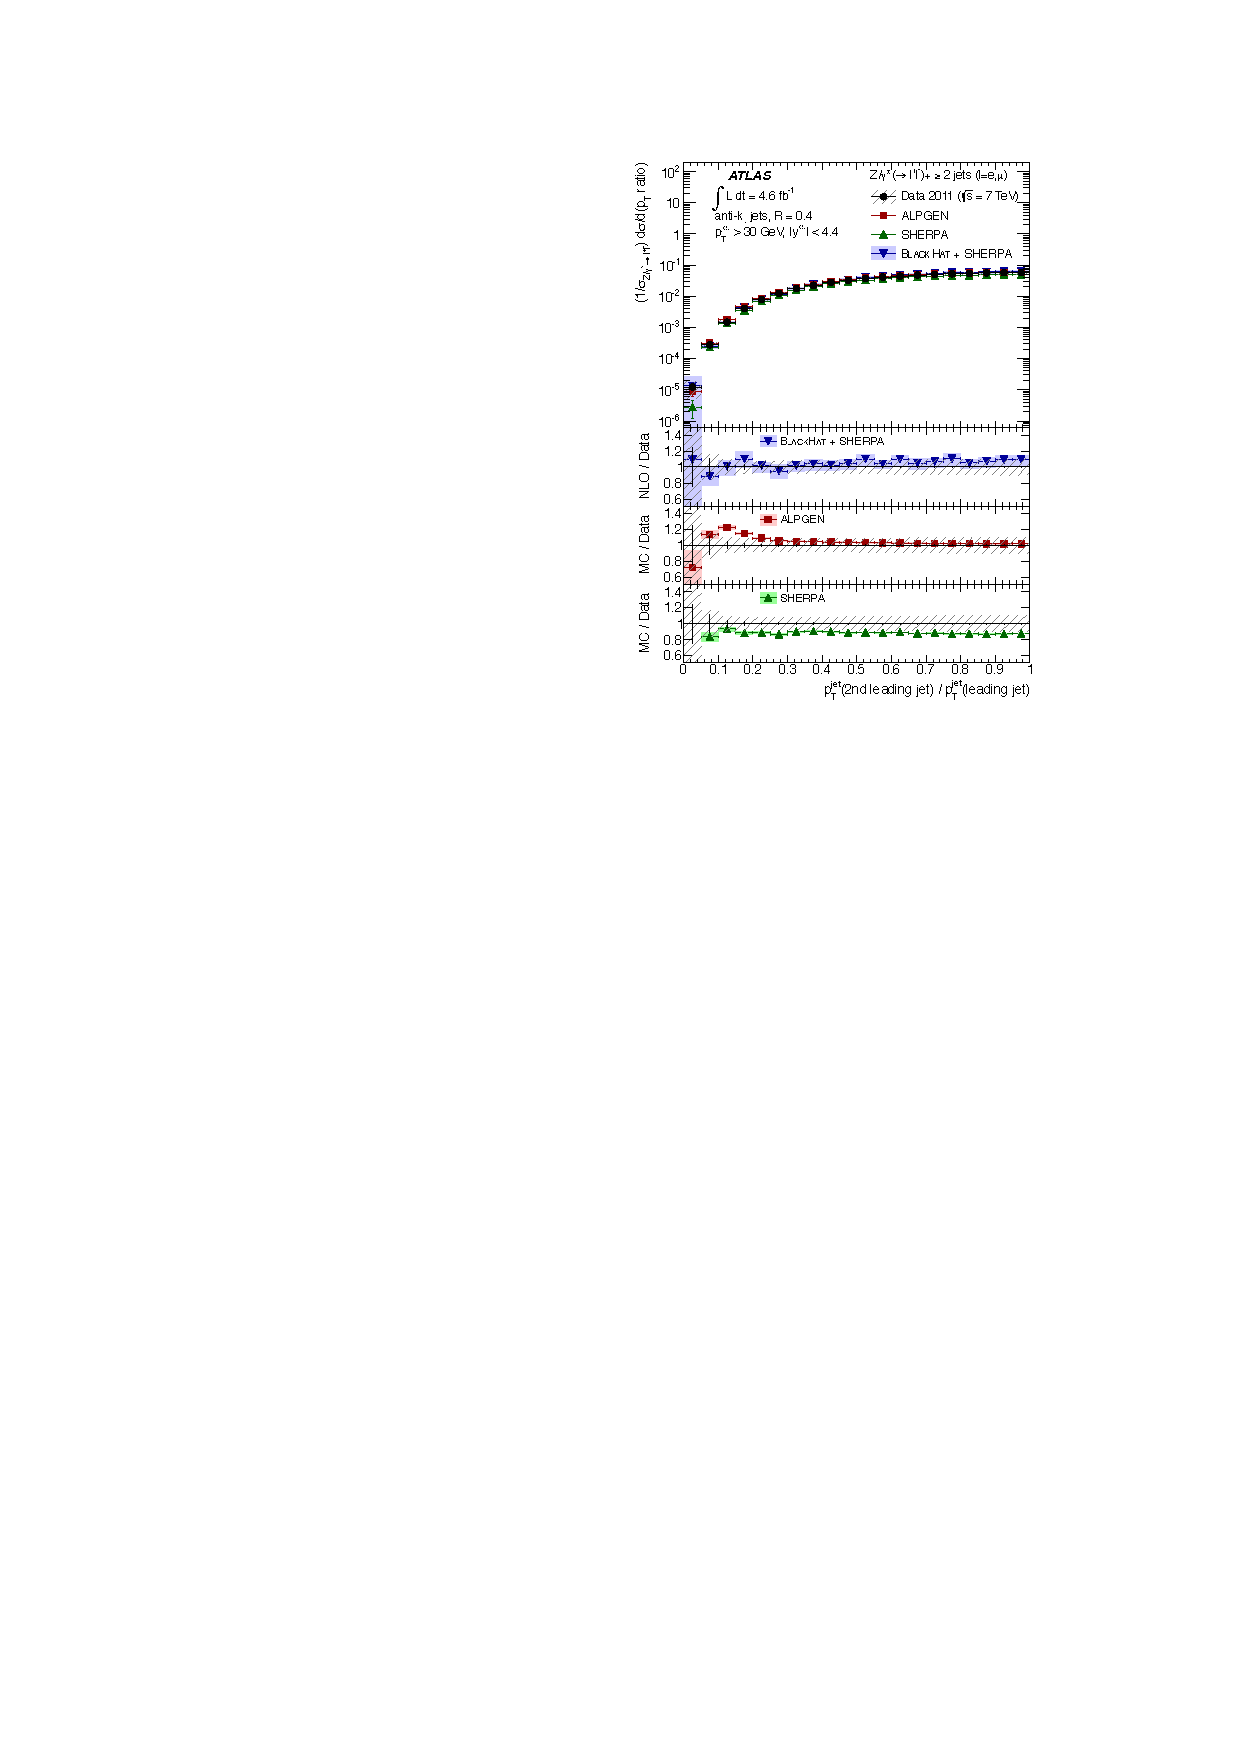
\includegraphics[width=\textwidth, height=1.2\textwidth]{Comparison_7b}
		    \caption{}
		    \label{fig:MC_ATLAS_7b}
		  \end{subfigure}
		  \caption{These plots show the differential cross section in the ratio of the leading
		     and second leading jet in $p_T$ from (a) HEJ and (b) other
		    theory descriptions and data~\cite{Aad:2013ysa}.}
		  \label{fig:ATLAS_7b}
		\end{figure}

	\subsection{$\zg$+Jets at the CMS Experiment}
		\label{sub:CMS}

		We now compare to data from a CMS analysis of events with a $\zg$ boson produced
		in association with jets~\cite{Khachatryan:2014zya}.  We show, for comparison,
		the plots from that analysis which contain theoretical predictions from
		Sherpa~\cite{Gleisberg:2008ta,Hoeche:2012yf}, Powheg~\cite{Alioli:2010qp} and
		MadGraph~\cite{Alwall:2014hca}.The cuts used for this analysis are summarised in
		tab.~\eqref{tab:cmscuts}.

		\begin{table}[hbt]
		  \centering
		  \begin{tabular}{|l|c|}
		    \hline
		    Lepton Cuts & $p_{T\ell}>20$~GeV, \; $|\eta_\ell|<2.4$ \\
		    &\; $71$~GeV $\leq m^{\ell^+\ell^-} \leq
		      111$~GeV \\ \hline
		    Jet Cuts (anti-$k_T$, 0.5) & $p_{Tj}>30$~GeV, \; $|y_j|<2.4$ \\
		    & $\Delta R^{j\ell} >0.5$ \\
		\hline
		  \end{tabular}
		  \caption{Cuts applied to theory simulations in the CMS
		    $Z$-plus-jets analysis results shown in
		    Figs.~\eqref{fig:CMS_2a}--\eqref{fig:CMS_3c}}
		  \label{tab:cmscuts}
		\end{table}

		As in the previous section, any jet which failed the final isolation cut was
		removed from the event, but the event itself is kept provided there are a
		sufficient number of other jets present.  The main difference to these cuts and
		those of ATLAS in the previous section is that the jets are required to be more
		central; $|\eta|<2.4$ as opposed to $|y|<4.4$.  This allows less room for
		evolution in rapidity; however, HEJ predictions are still relevant in this
		scenario.  Once again, the central values are given by $\mu_F=\mu_R=H_T/2$ with
		theoretical uncertainty bands determined by varying these independently by
		factors of two around this value.  HEJ events always contain a minimum of two
		jets and therefore here we only compare to the distributions for an event sample
		with at least two jets or above.

		We begin in Fig.~\eqref{fig:CMS_2a} by showing the inclusive jet rates for these
		cuts.  The HEJ predictions give a good description, especially for the 2- and
		3-jet inclusive rates in this narrower phase space. The uncertainty bands are
		larger for HEJ than for the Sherpa and Powheg predictions due to our LO matching
		prescription (those for Madgraph are not shown).

		In Figs.~\eqref{fig:CMS_3b}--~\eqref{fig:CMS_3c}, we show the transverse momentum
		distributions for the second and third jet respectively (the leading jet
		distribution was not given for inclusive dijet events).  Beginning with the
		second jet in Fig.~\eqref{fig:CMS_3b}, we see that the HEJ predictions overshoot
		the data at large transverse momentum.  In this region, the non-FKL matched
		components of the HEJ description become more important and these are not
		controlled by the high-energy resummation.  The HEJ predictions are broadly
		similar to Powheg's $Z$-plus-one-jet NLO calculation matched with the Pythia
		parton shower.  In contrast, Sherpa's prediction significantly undershoots the
		data at large transverse momentum.  Here the Madgraph prediction gives the best
		description of the data.

		% Fig.~\eqref{fig:CMS_3c} shows the transverse momentum distribution of the third
		% jet in this data sample.  Here, the shape of HEJ prediction compared to the data
		% increases with transverse momentum, but the slope is not great and the deviation
		% is never greater than 20\%.  Both the Sherpa and Powheg predictions show greater
		% deviations.  This is not surprising for the Powheg prediction since it only
		% contains a hard-scattering matrix element for up to two jets.  The Madgraph
		% prediction again performs very well until the last bin.

		Fig.~\eqref{fig:CMS_3c} shows the transverse momentum distribution of the third
		jet in this data sample.  Here, the ratio of the HEJ prediction to data shows a
		linear increase with transverse momentum (until the last bin where all the
		theory predictions show the same dip).  Both the Sherpa and Powheg predictions
		show similar deviations for this variable while the Madgraph prediction again
		performs very well.

		% Finally, we show the transverse momentum distribution of the fourth jet in
		% Fig.~\eqref{fig:CMS_3d}.

		\begin{figure}[h]
		  \centering
		  \begin{subfigure}[b]{0.46\textwidth}
		    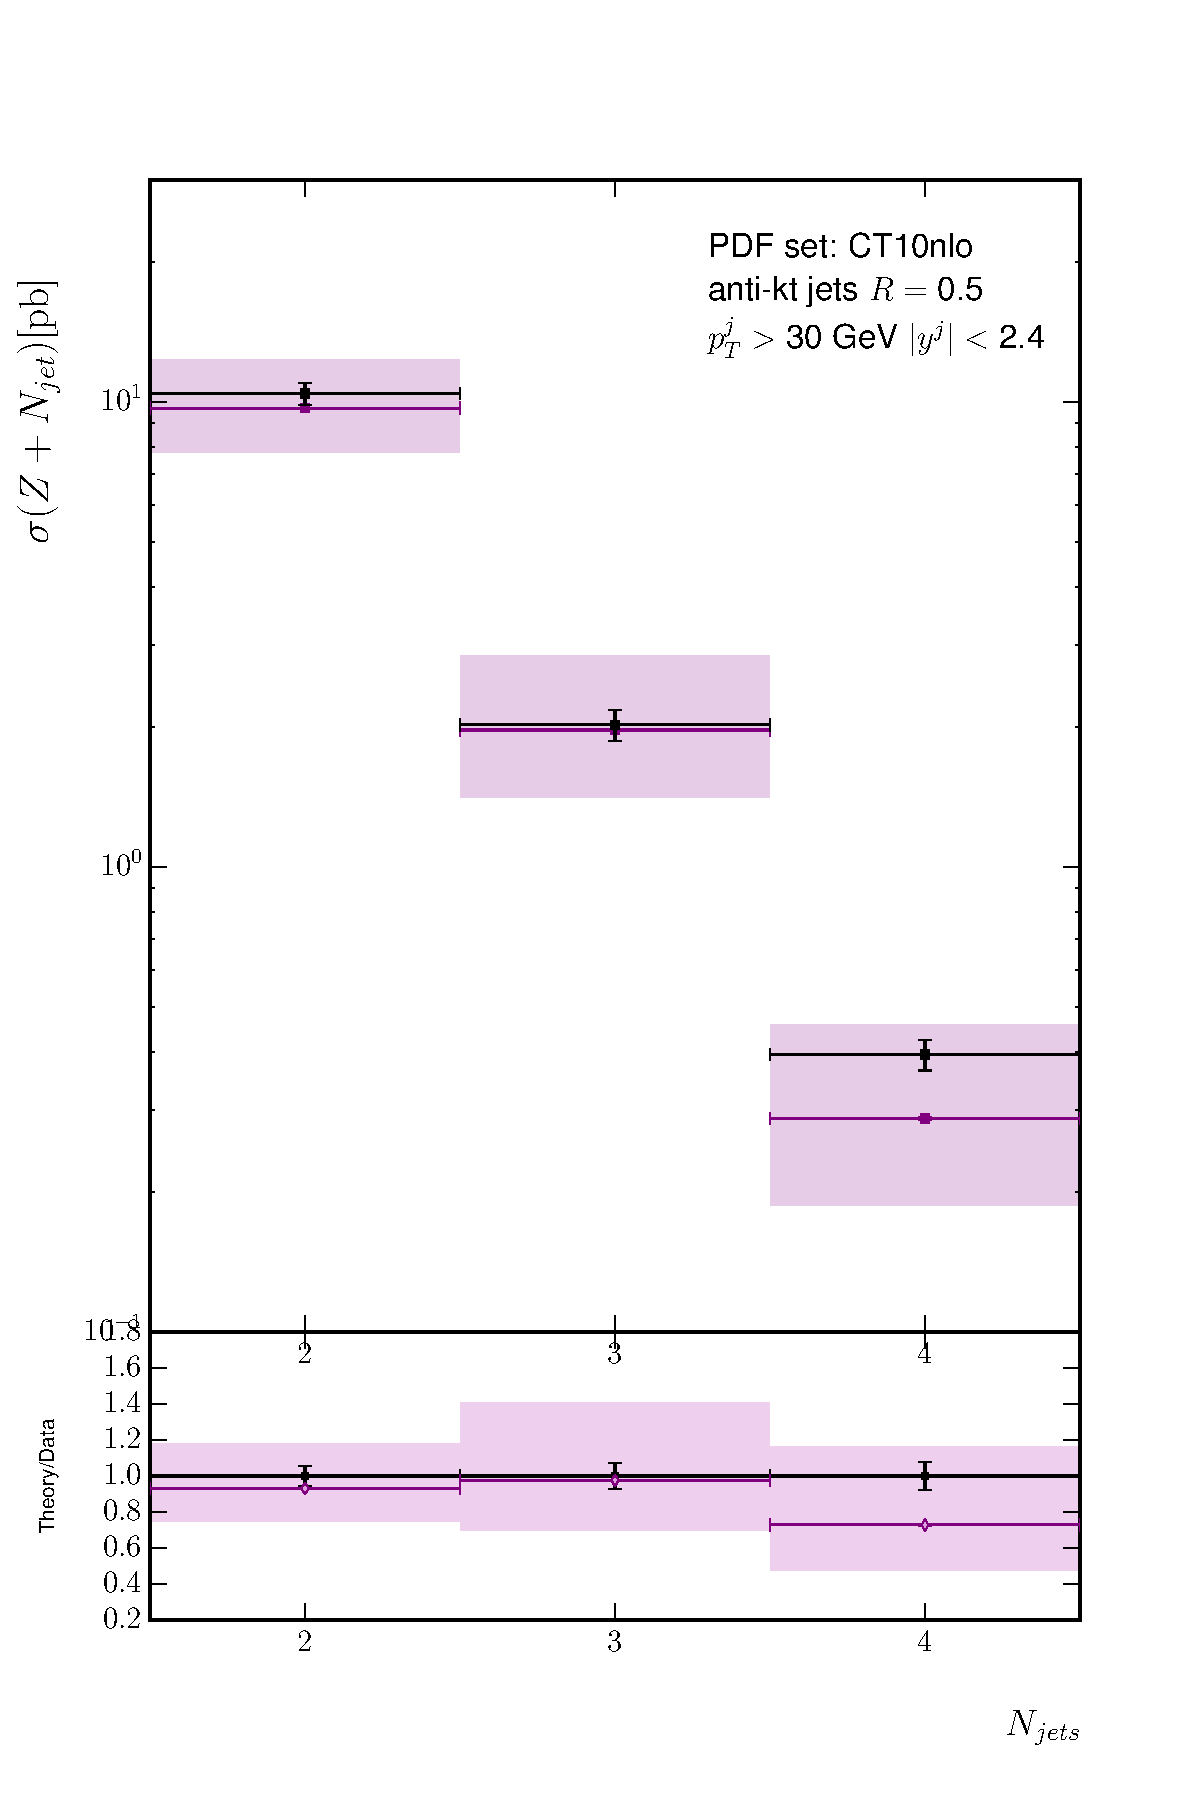
\includegraphics[width=\textwidth, height=1.2\textwidth]{CMS_Z_2a}
		    \caption{}
		    \label{fig:HEJ_CMS_2a}
		  \end{subfigure}
		  ~
		  \begin{subfigure}[b]{0.48\textwidth}
		    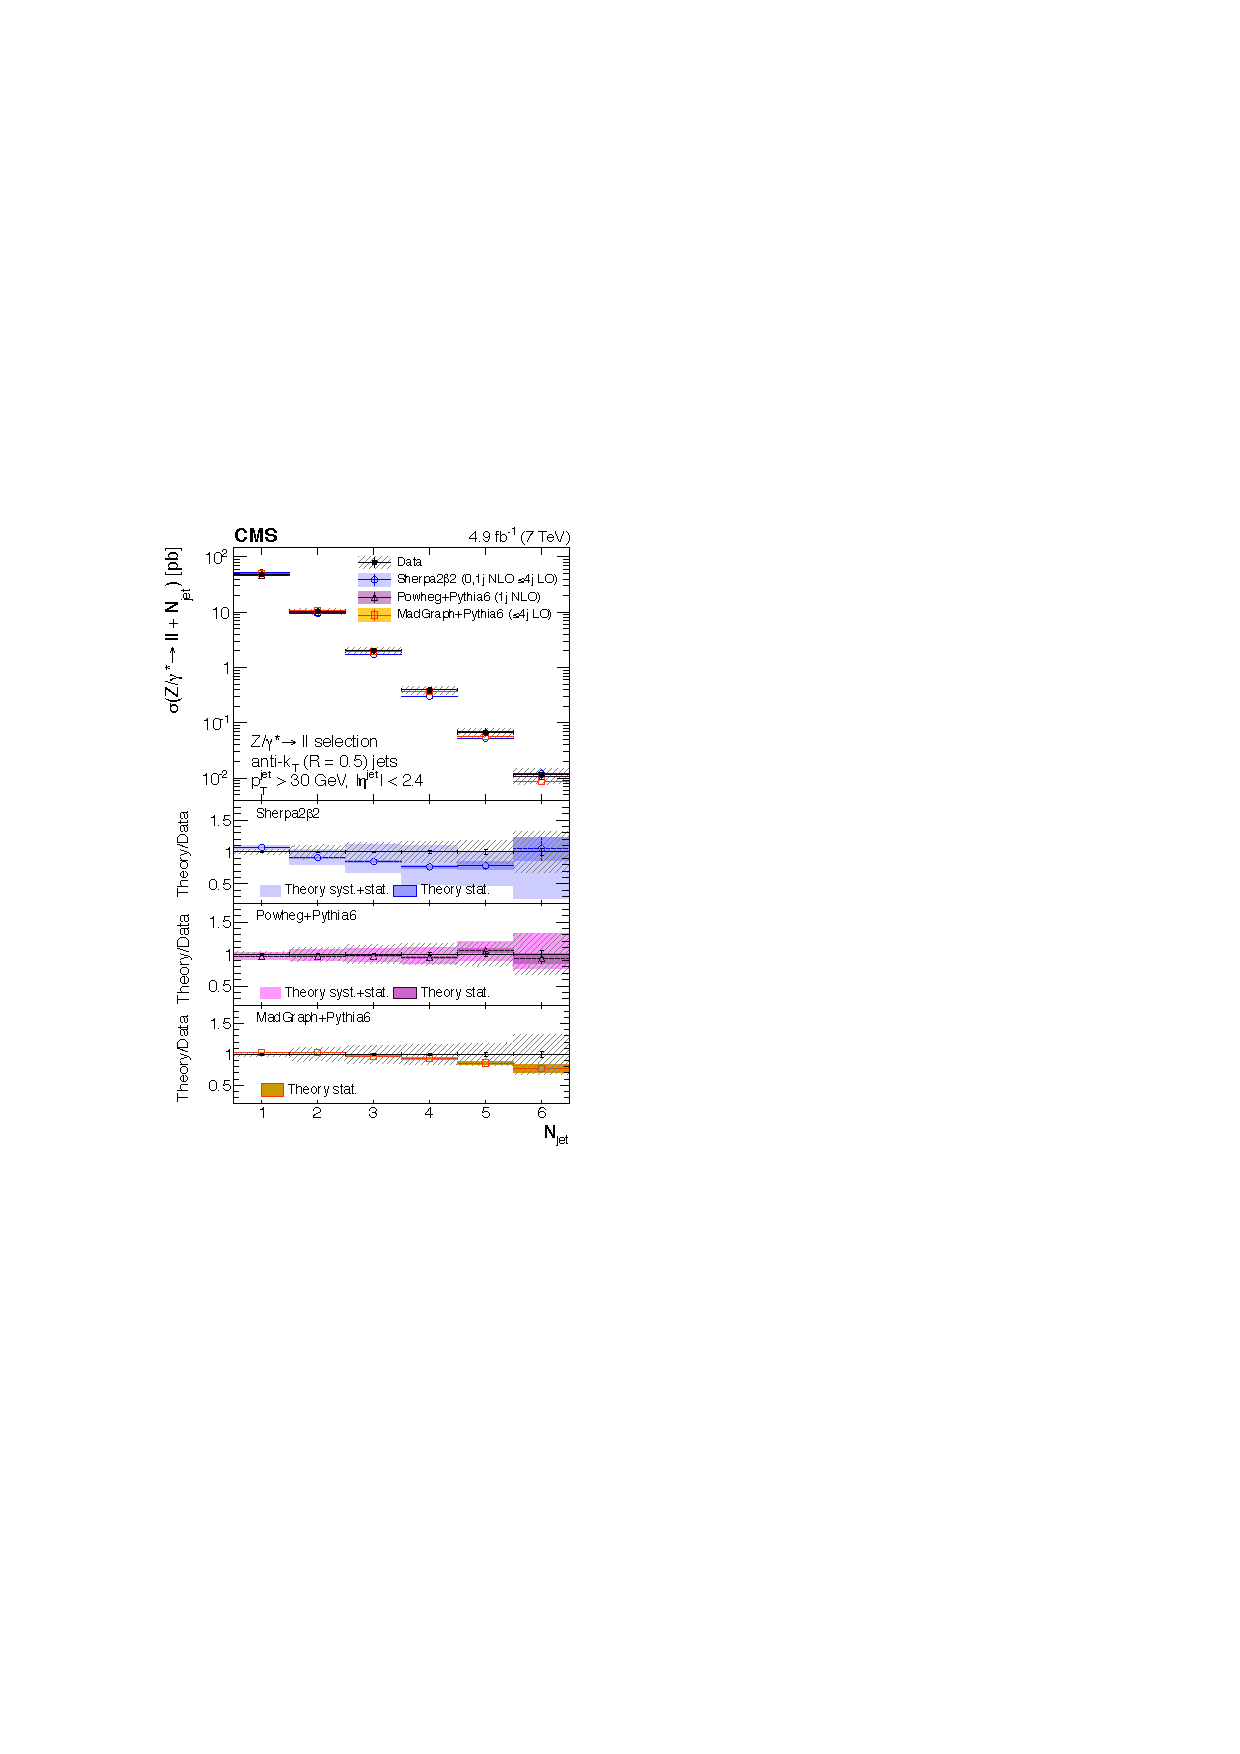
\includegraphics[width=\textwidth, height=1.2\textwidth]{ComparisonCMS_2a}
		    \caption{}
		    \label{fig:MC_CMS_2a}
		  \end{subfigure}
		  \caption{The inclusive jet rates as given by (a) the HEJ description and (b)
		    by other theoretical descriptions, both plots compared to the CMS data in~\cite{Khachatryan:2014zya}.}
		  \label{fig:CMS_2a}

		  \begin{subfigure}[b]{0.46\textwidth}
		    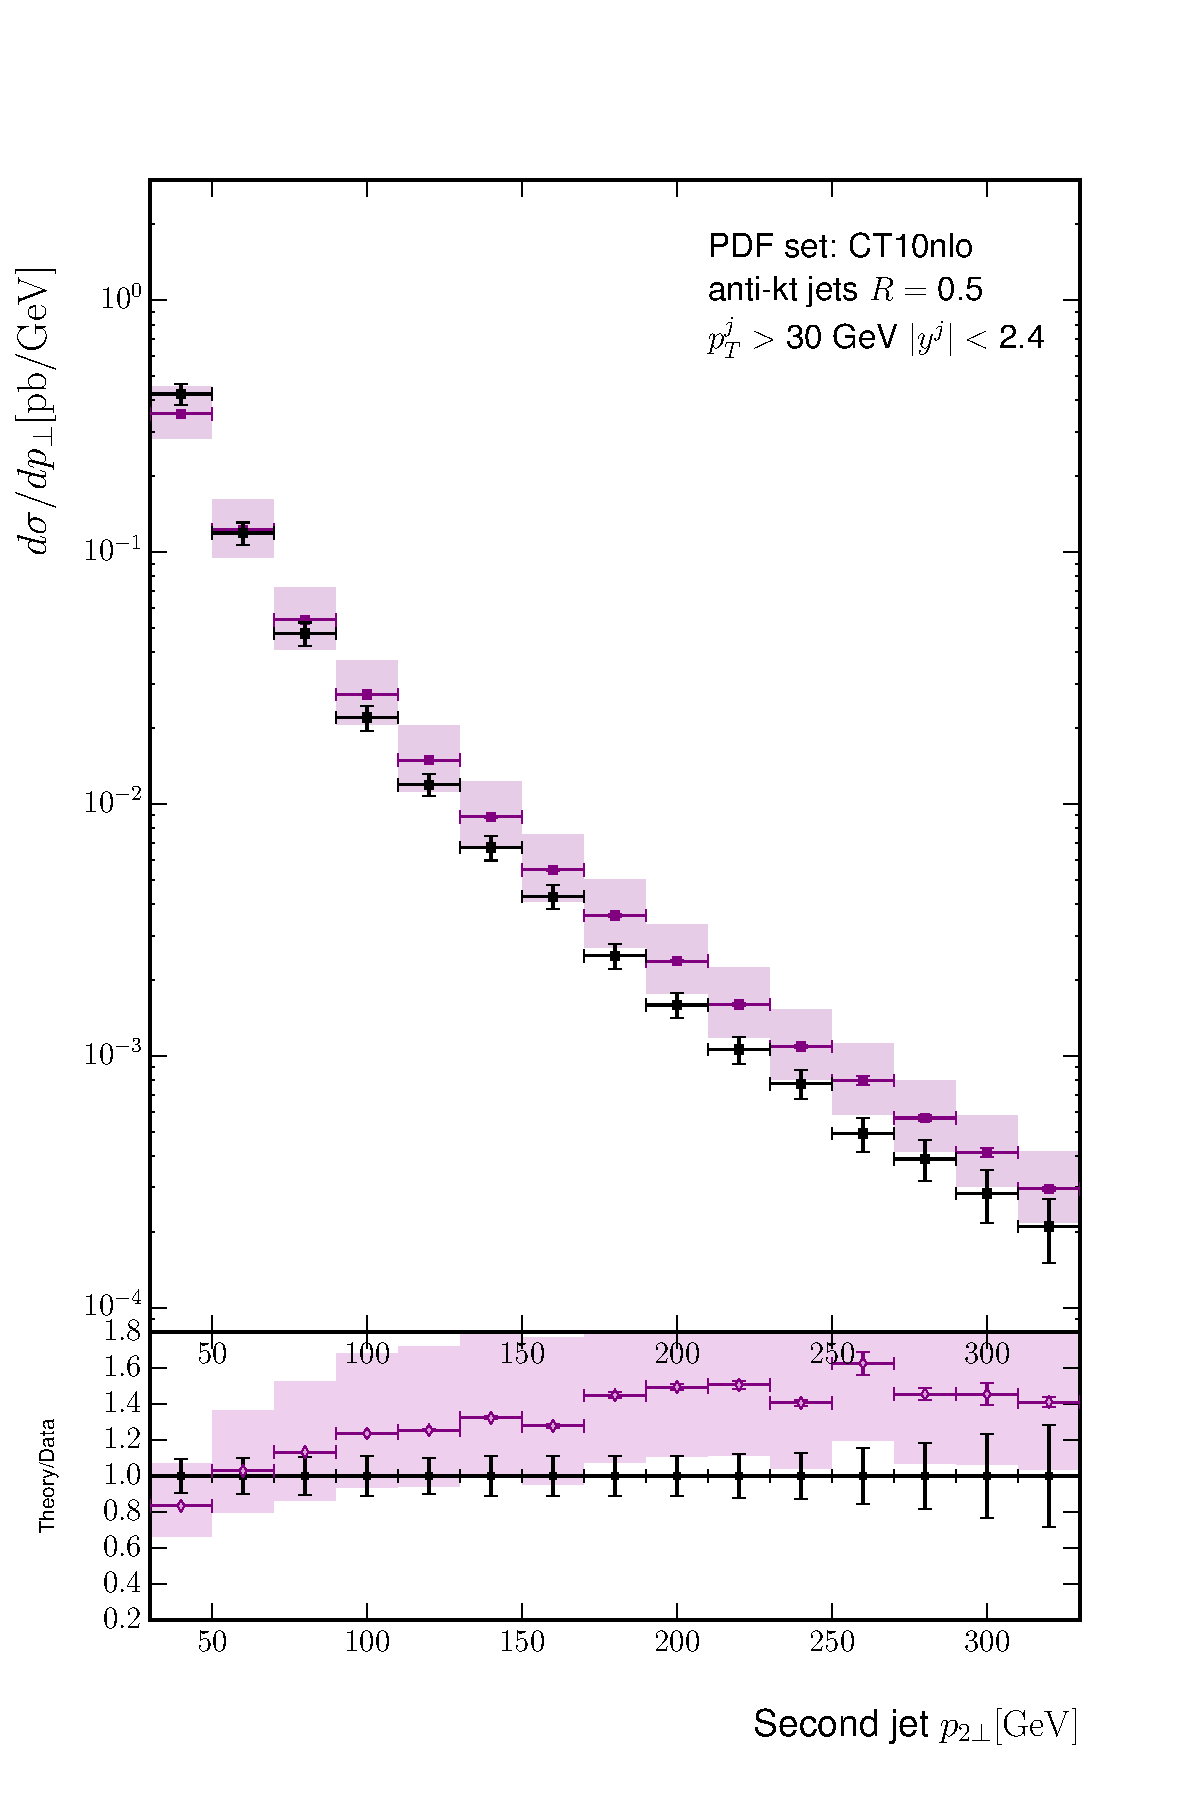
\includegraphics[width=\textwidth, height=1.2\textwidth]{CMS_Z_3b}
		    \caption{}
		    \label{fig:HEJ_CMS_7b}
		  \end{subfigure}
		  ~
		  \begin{subfigure}[b]{0.48\textwidth}
		    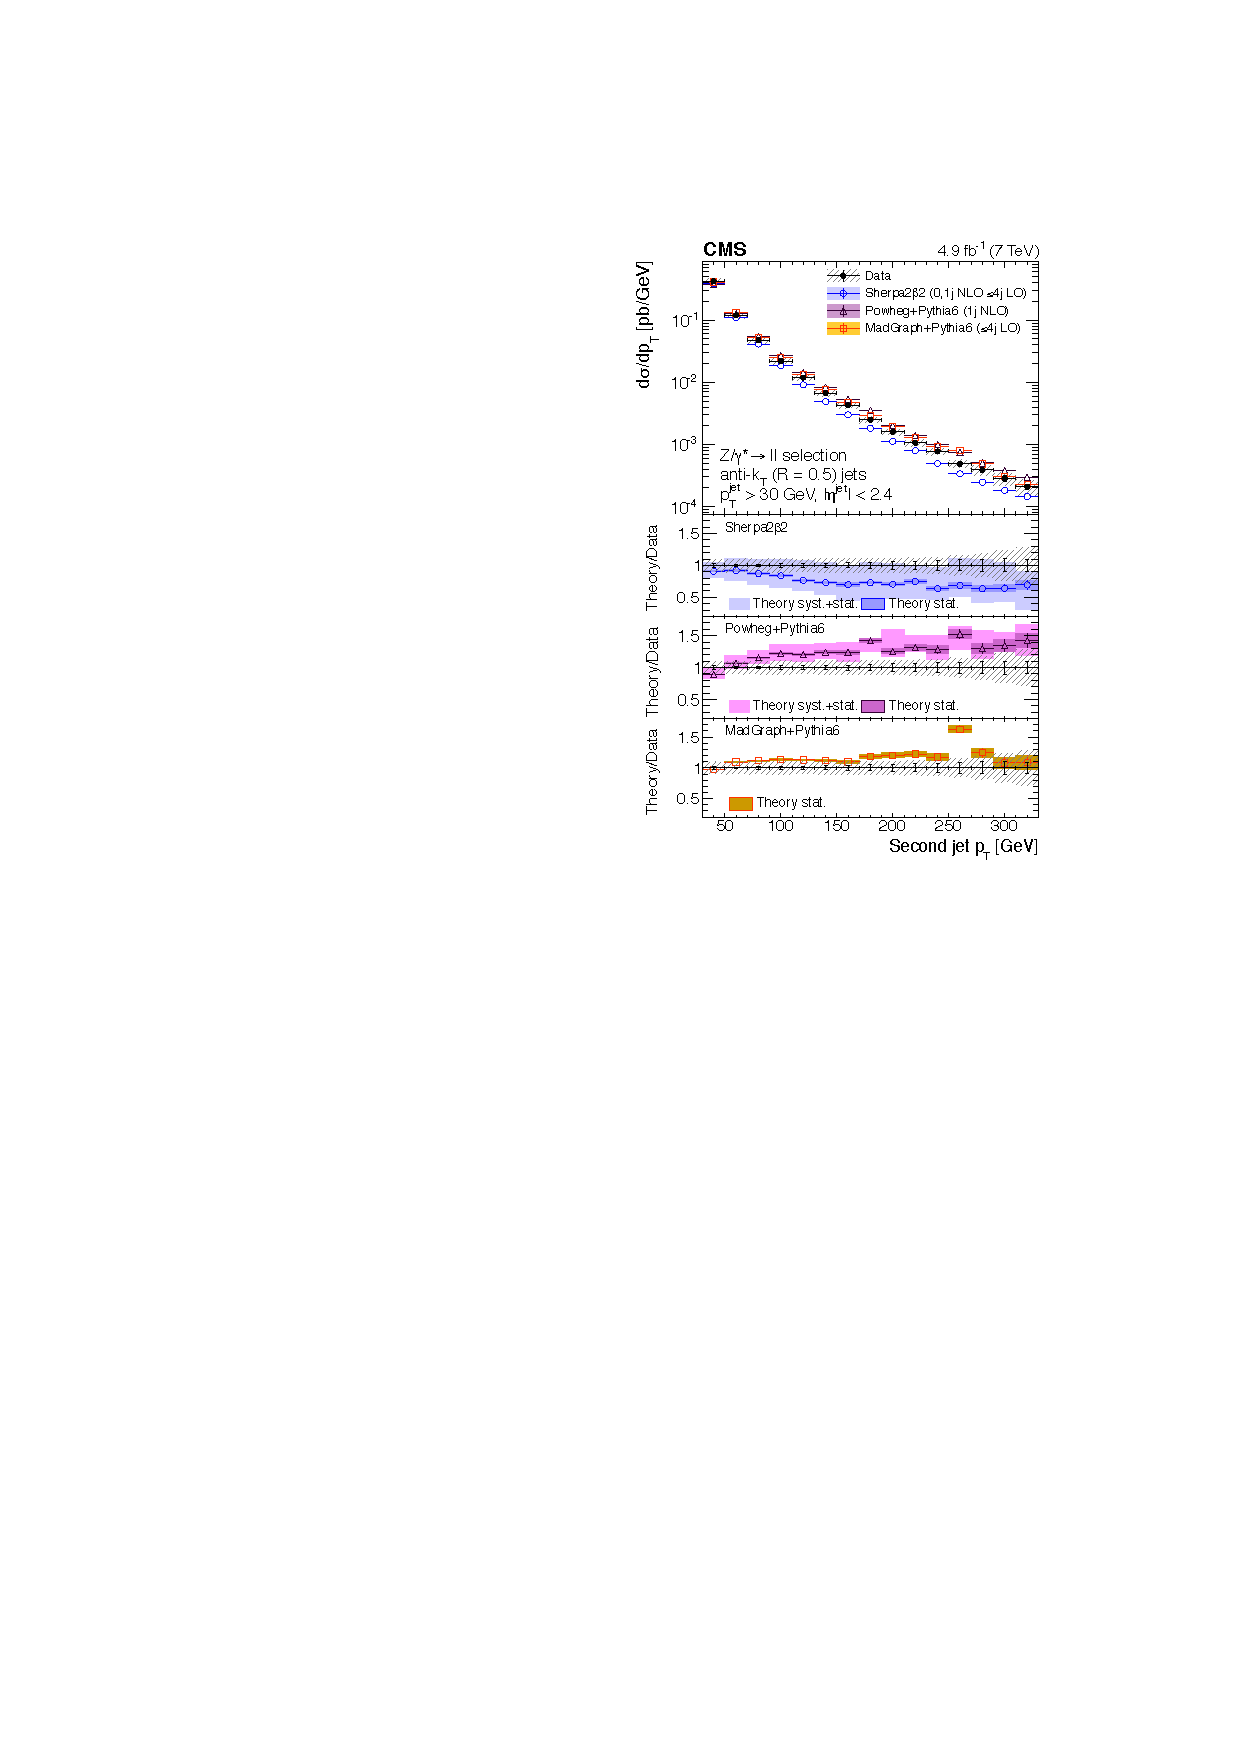
\includegraphics[width=\textwidth, height=1.2\textwidth]{ComparisonCMS_3b}
		    \caption{}
		    \label{fig:MC_CMS_7b}
		  \end{subfigure}
		  \caption{The transverse momentum distribution of the second hardest jet in
		    inclusive dijet events in~\cite{Khachatryan:2014zya}, compared to (a) the
		    predictions from HEJ and (b) the predictions from other theory descriptions.}
		  \label{fig:CMS_3b}
		\end{figure}

		\begin{figure}[H]
		  \centering
		  \begin{subfigure}[b]{0.46\textwidth}
		    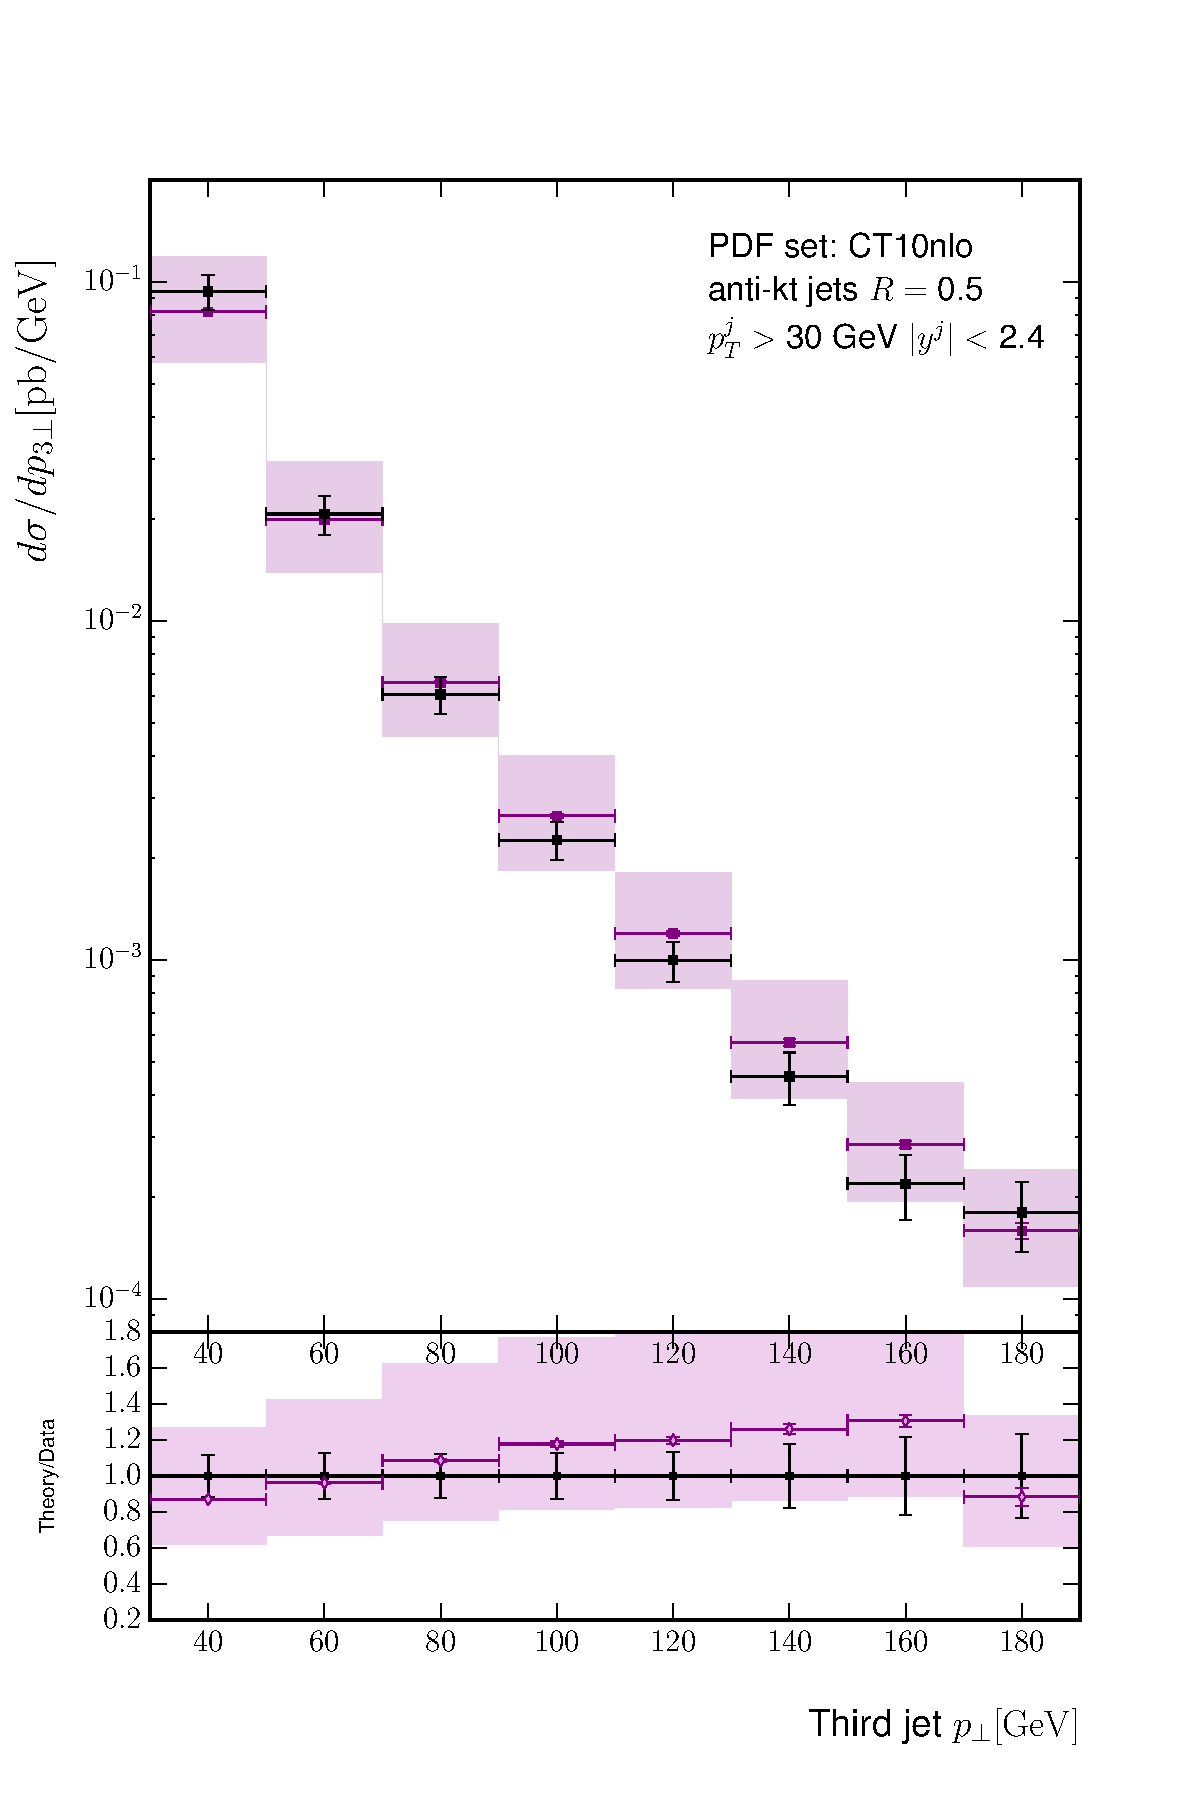
\includegraphics[width=\textwidth, height=1.2\textwidth]{CMS_Z_3c}
		    \caption{}
		    \label{fig:HEJ_CMS_7b}
		  \end{subfigure}
		  ~
		  \begin{subfigure}[b]{0.48\textwidth}
		    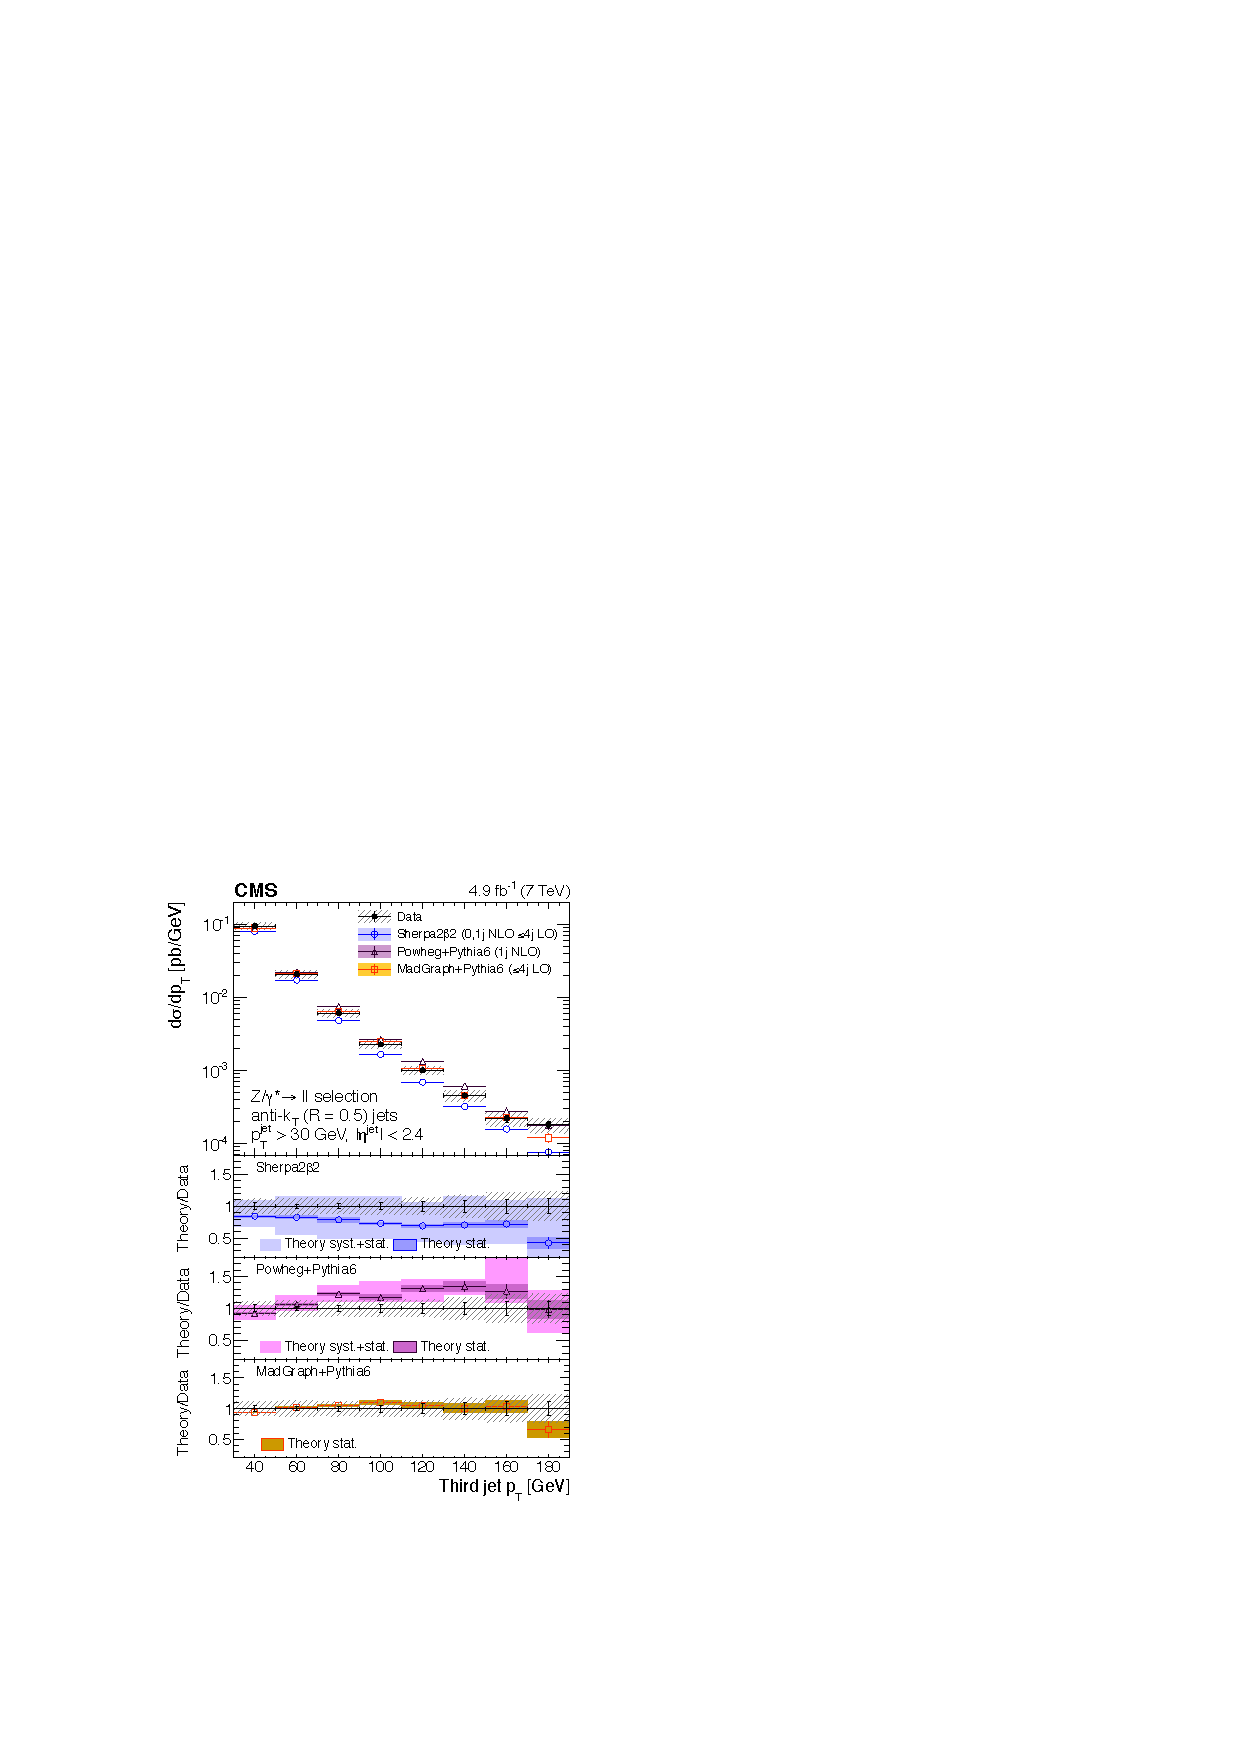
\includegraphics[width=\textwidth, height=1.2\textwidth]{ComparisonCMS_3c}
		    \caption{}
		    \label{fig:MC_CMS_7b}
		  \end{subfigure}
		  \caption{The transverse momentum distribution of the third hardest jet in
		    inclusive dijet events in~\cite{Khachatryan:2014zya}, compared to (a) the
		    predictions from HEJ and (b) the predictions from other theory descriptions.}
		  \label{fig:CMS_3c}
		\end{figure}

